%!TEX root = ./main.tex

%%**************************************************************
%%
%% DHBW Heidenheim - Template for Bachelor Thesis
%%
%% For further information see REAMDME.md
%%
%%**************************************************************

%!TEX root = ../main.tex

% show warning for old LaTeX syntax
\RequirePackage[l2tabu, orthodox]{nag}

\documentclass[
	pdftex,
	oneside,  
	12pt,			    % fontsize
	parskip=half,		    % Space (in lines) between paragraphs
	headheight = 12pt,    % Header hight
	headsepline,		    % Line after header
	footheight = 16pt,	    % Footer height
	footsepline,		    % Line before footer
	abstracton,		    % Abstract headline
	DIV=calc,		    % Calculate print space
	BCOR=8mm,		    % BCOR settings (Bindekorrektur)
	headinclude=false,   % Exclude header from print space
	footinclude=false,	    % Exclude footer from print space
	listof=totoc,		    % Show List of Figures/Tables in Contents
	toc=bibliography,	    % Show Bibliography in Contents
]{scrreprt}	                     % Koma-Script report-class, long document: scrreprt, short document: scrbook

\usepackage{xstring}
\usepackage[utf8]{inputenc}
\usepackage[T1]{fontenc}

% iflang command definition
\newcommand{\iflang}[2]{%
  \IfStrEq{\documentLanguage}{#1}{#2}{}
}

% ifDocType comand definition
\newcommand{\ifDocType}[2]{%
  \IfStrEq{\documentType}{#1}{#2}{}
}

% Include main settings
%!TEX root = ./main.tex

%%**************************************************************
%%
%% DHBW Heidenheim - Template for Bachelor Thesis
%%
%% For further information see REAMDME.md
%%
%%**************************************************************

%!TEX root = ../main.tex

% show warning for old LaTeX syntax
\RequirePackage[l2tabu, orthodox]{nag}

\documentclass[
	pdftex,
	oneside,  
	12pt,			    % fontsize
	parskip=half,		    % Space (in lines) between paragraphs
	headheight = 12pt,    % Header hight
	headsepline,		    % Line after header
	footheight = 16pt,	    % Footer height
	footsepline,		    % Line before footer
	abstracton,		    % Abstract headline
	DIV=calc,		    % Calculate print space
	BCOR=8mm,		    % BCOR settings (Bindekorrektur)
	headinclude=false,   % Exclude header from print space
	footinclude=false,	    % Exclude footer from print space
	listof=totoc,		    % Show List of Figures/Tables in Contents
	toc=bibliography,	    % Show Bibliography in Contents
]{scrreprt}	                     % Koma-Script report-class, long document: scrreprt, short document: scrbook

\usepackage{xstring}
\usepackage[utf8]{inputenc}
\usepackage[T1]{fontenc}

% iflang command definition
\newcommand{\iflang}[2]{%
  \IfStrEq{\documentLanguage}{#1}{#2}{}
}

% ifDocType comand definition
\newcommand{\ifDocType}[2]{%
  \IfStrEq{\documentType}{#1}{#2}{}
}

% Include main settings
\input{settings/main} 

% Include document settings
\input{settings/document}

% Load language specific Strings
\input{lang/\documentLanguage}

% Load language specific babel package
\iflang{de}{\usepackage[english, ngerman]{babel}}
\iflang{en}{\usepackage[ngerman, english]{babel}} 

% Add comment feature
\newcommand{\comment}[1]{\par {\bfseries \color{blue} #1 \par}}


%%%%%%% Package Includes %%%%%%%

\usepackage[margin=\margin,foot=1cm]{geometry}
\usepackage[activate]{microtype}                                         
\usepackage[onehalfspacing]{setspace}
\usepackage{makeidx}
\usepackage[autostyle=true,german=quotes]{csquotes}
\usepackage{longtable}
\usepackage{enumitem}	                                                 
\usepackage{graphicx}
\usepackage{pdfpages}                                                         
\usepackage{xcolor} 	                                                    
\usepackage{float}
\usepackage{array}
\usepackage{calc}		                         
\usepackage[right]{eurosym}
\usepackage{wrapfig}
\usepackage{pgffor}                                                             
\usepackage[perpage, hang, multiple, stable]{footmisc}  
\usepackage[printonlyused]{acronym}                                 
\usepackage{listings}
\usepackage[obeyFinal,backgroundcolor=yellow,linecolor=black]{todonotes}
\usepackage{rotating}
\usepackage{lscape}
\usepackage{amsmath}
\usepackage{amssymb}
\usepackage{\documentFont}
\usepackage[%
	pdftitle={\documentTitle},
	pdfauthor={\documentAuthor},
	pdfsubject={\documentType},
	pdfcreator={pdflatex, LaTeX with KOMA-Script},
	pdfpagemode=UseOutlines,       % Show Contents while opening
	pdfdisplaydoctitle=true, 		% Show document title instead of file name
	pdflang={\documentLanguage}, % Document language
]{hyperref}
\usepackage{bookmark}
\usepackage[nonumberlist,toc]{glossaries}

% Load colors
\defineColors{}

% Set Titel, Autor and Date
\title{\documentTitle}
\author{\documentAuthor}
\date{\datum}


% PDF link settings
\hypersetup{%
	colorlinks=true, 		
	linkcolor=LinkColor, 	
	citecolor=LinkColor,
	filecolor=LinkColor,
	menucolor=LinkColor,
	urlcolor=LinkColor,
	linktocpage=true, 
	bookmarksnumbered=true 
}

% Captions fontsize
\addtokomafont{caption}{\small}

% Bibliographie settings
\iflang{de}{%
\usepackage[
	backend=biber,		% recommended. Alternative: bibtex
	bibwarn=true,
	bibencoding=utf8,	         % If .bib file is encoded with utf8, otherwise ascii
	sortlocale=de_DE,
	style=\quoteStyle,
]{biblatex}
}
\iflang{en}{%
\usepackage[
	backend=biber,		% recommended. Alternative: bibtex
	bibwarn=true,
	bibencoding=utf8,        % If .bib file is encoded with utf8, otherwise ascii
	sortlocale=en_US,
	style=\quoteStyle,
]{biblatex}
}

\addbibresource{bibliographie.bib}

% Hurenkinder und Schusterjungen verhindern
% http://projekte.dante.de/DanteFAQ/Silbentrennung
\clubpenalty = 10000 % schließt Schusterjungen aus (Seitenumbruch nach der ersten Zeile eines neuen Absatzes)
\widowpenalty = 10000 % schließt Hurenkinder aus (die letzte Zeile eines Absatzes steht auf einer neuen Seite)
\displaywidowpenalty=10000

% Graphicspath
\graphicspath{{images/}}

% frequently used programing languages
\lstloadlanguages{PHP,Python,Java,C,C++,bash,SQL}

\listingsettings{}
% Rename Listings
\renewcommand\lstlistingname{\listingPhrase}
\renewcommand\lstlistlistingname{\listListingPhrase}
\def\lstlistingautorefname{\authorListingPhrase}

% JSON Listings
\colorlet{punct}{red!60!black}
\definecolor{background}{HTML}{EEEEEE}
\definecolor{delim}{RGB}{20,105,176}
\colorlet{numb}{magenta!60!black}

\lstdefinelanguage{json}{
    basicstyle=\normalfont\ttfamily,
    numbers=left,
    numberstyle=\scriptsize,
    stepnumber=1,
    numbersep=8pt,
    showstringspaces=false,
    breaklines=true,
    frame=lines,
    backgroundcolor=\color{background},
    literate=
     *{0}{{{\color{numb}0}}}{1}
      {1}{{{\color{numb}1}}}{1}
      {2}{{{\color{numb}2}}}{1}
      {3}{{{\color{numb}3}}}{1}
      {4}{{{\color{numb}4}}}{1}
      {5}{{{\color{numb}5}}}{1}
      {6}{{{\color{numb}6}}}{1}
      {7}{{{\color{numb}7}}}{1}
      {8}{{{\color{numb}8}}}{1}
      {9}{{{\color{numb}9}}}{1}
      {:}{{{\color{punct}{:}}}}{1}
      {,}{{{\color{punct}{,}}}}{1}
      {\{}{{{\color{delim}{\{}}}}{1}
      {\}}{{{\color{delim}{\}}}}}{1}
      {[}{{{\color{delim}{[}}}}{1}
      {]}{{{\color{delim}{]}}}}{1},
}

% Spaces in tables
\setlength{\tabcolsep}{\tableColumnMargin}
\renewcommand{\arraystretch}{\tableRowMargin}


\input{content/glossary}

\begin{document}

	% Cover
	\begin{spacing}{1}
		\input{ads/cover}
	\end{spacing}
	\newpage

	\pagenumbering{Roman}

	% Restriction notices
	%\input{ads/restrictionNotices}
	%\newpage

	% Declaration
	%!TEX root = ../main.tex

\thispagestyle{empty}

\section*{\declarationPhrase}

\vspace*{2em}

\iflang{de}{%
  Ich versichere hiermit, dass ich die vorliegende Arbeit mit dem Thema: {\itshape \documentTitle } 
  selbstständig verfasst und  keine anderen als die angegebenen Quellen und Hilfsmittel benutzt habe. 
  Ich versichere zudem, dass die eingereichte elektronische Fassung mit der gedruckten Fassung 
  übereinstimmt. 
}


\iflang{en}{%
  Hereby we solemnly declare:
  \begin{enumerate}
  \item that this document, titled {\itshape \documentTitle } is entirely the product of our 
            own scholarly work, unless otherwise indicated in the text or references, or acknowledged below;
  \item We have indicated the thoughts adopted directly or indirectly from other sources at the appropriate 
            places within the document;
  \item This document has not been submitted either in whole or part, for a degree at this or 
            any other university or institution;
  \item We have not published this document in the past.
  \end{enumerate}
  We are aware that a dishonest declaration will entail legal consequences.
}

\vspace{3em}

\releaseLocation, \releaseDate
\vspace{4em}

\rule{6cm}{0.4pt}\\
\documentAuthor

	\newpage

	% Abstract
	%!TEX root = ../main.tex

\pagestyle{empty}

% override abstract headline

%\renewcommand{\abstractname}{Zusammenfassung}
%
%\begin{abstract}
%
%lorem ipsum
%
%\end{abstract}

\renewcommand{\abstractname}{Abstract}

\begin{abstract}

These days Machine Learning, Neural Networks or Data Mining are common buzzwords
in the world of computer science. But a lot of people do not know what they are actually
talking about, when using these kind of words. Therefore it makes sense to learn about
neural networks and machine learning in general during the course of a masters degree in
information technology. Fortunately there are many data sets online to use for analysis
to get a basic understanding of the topic at hand. The European Soccer Database from
Kaggle [6] is such a data set.
During the team project of the information systems master at the Technische Hochschule
Ulm it was our task to use the european soccer database for analytics in order to be able
to predict the outcome of soccer matches.
From the database we extracted several different features, like amount of goals shot
by each team, amount of wins, draws and losses for each team as well as shot-accuracy
and shot-efficiency per team and the overall ball possession of each soccer-team per match.
Using an algorithm which we adapted for our special data [2] we created a sliding window
which aggregates the extracted features over the last 10 soccer-games for each match
in the database in chronological order. Because a lot of data samples in the database
were incomplete regarding some of the extracted features, we created 5 different versions
of the sliding window. Each containing a different amount of features and therefore a
different amount of data samples. This gives us the possibility to test classifiers with
various different models and later pick the solution that works best. The sliding window
option 1 uses the least amount of features (13 features) and has the highest number of data
samples (20823 data samples). Option 2 has 21 features and 7033 data samples, option 3
uses 29 features and 7033 samples, option 4 contains 25 features and 6996 samples and
option 5 has the most features (33) and 6996 data samples.
We used the 5 sliding window options to train and test various classifiers such as a
Decision Tree, a Multi-Layer Perceptron and various different basic sequential neural nets.
For the Decision Tree and the Multi-Layer Perceptron we used the scikit-learn API. For
the basic sequential neural nets we used the Tensorflow/Keras framework, which is state
of the art when doing data analytics tasks.
The decision tree using the first sliding window option and a depth of 4 gives us a testaccuracy
of 52,95\%. The Multi-Layer Perceptron uses the sliding window option 1 aswell
and has a test-accuracy of 53,45\%. It has 2 hidden layers with 52 and 32 neurons. The
best version of the Keras Sequential Neural Network was trained with sliding window
option 3, has 2 hidden layers (21, 21 neurons) and a test-accuracy of 56,25%. It is also the
best classifier in general we were able to find until now. At first sight model accuracies
barely over 50\% don’t seem very good, but considering that the home team has a base
chance of 46\% to win the match and soccer is still a gambling game up to some point
those accuracies aren’t too bad at all.
Nevertheless, the team will continue its work on the project striving for better models
by using additional features and varying the amount of features, adapting the split of
training- and test-data, trying other kinds of classifiers and tweaking the existing models
by changing parameters and input functions.


\end{abstract}
	\newpage

        % only page number in footer
	\pagestyle{plain}
	
	% space bevore chapter headline
	\RedeclareSectionCommand[beforeskip=\chapterMargin]{chapter}

	% Contents
	\begin{spacing}{1.1}
		\begingroup
		
		        % set subchapter depth
			\setcounter{tocdepth}{1}
			
			\tableofcontents
			\clearpage
		\endgroup
	\end{spacing}
	\newpage

	% Acronyms
	%\cleardoublepage
       % \input{content/acronyms}

	% List of Figures
	\cleardoublepage
	\listoffigures

	%List of Tables
	\cleardoublepage
	\listoftables

	% List of Listings
	\cleardoublepage
	\lstlistoflistings
	\cleardoublepage

	\pagenumbering{arabic}
	
	\pagestyle{headings}

	%Content
	\foreach \i in {01,02,03,04,05,06,07,08,09,...,99} {%
		\edef\FileName{content/chapter/\i .tex}%
			\IfFileExists{\FileName}{%
				\input{\FileName}
			}
			{%
%				No chapter available
			}
}

	\clearpage

	% Bibilography
	\cleardoublepage
	\printbibliography

	% Glossar
	\printglossary[style=altlist,title=\glossaryPhrase]
	
	% Appendix
	\clearpage
	\appendix
	% !TeX root = ../main.tex

\chapter{Appendix}
\section{Architectures for various neural nets}
\label{section:appendix_a}
\begin{longtable}{|l|l|l|l|l|l|l|}
\caption{Test Variation of Hidden-Layers and Neurons for Neural Nets} \\
\hline
\textbf{Name} & \textbf{Input} & \textbf{HLayer1} & \textbf{HLayer2} & \textbf{HLayer3} & \textbf{HLayer4} & \textbf{Output} \\ 
\hline
\endfirsthead
\hline
\textbf{Name} & \textbf{Input} & \textbf{HLayer1} & \textbf{HLayer2} & \textbf{HLayer3} & \textbf{HLayer4} & \textbf{Output} \\ 
\hline
\endhead
\multicolumn{7}{r}{continued on next page}\\
\endfoot
\hline
\multicolumn{7}{r}{end of table} \\
\endlastfoot
model01\_H1\_H & 13 & 13 & - & - & - & 3 \\ \hline
model02\_H1\_H & 21 & 21 & - & - & - & 3 \\ \hline
model03\_H1\_H & 29 & 29 & - & - & - & 3 \\ \hline
model04\_H1\_H & 25 & 25 & - & - & - & 3 \\ \hline
model05\_H1\_H & 33 & 33 & - & - & - & 3 \\ \hline
model01\_H1\_M & 13 & 9 & - & - & - & 3 \\ \hline
model02\_H1\_M & 21 & 12 & - & - & - & 3 \\ \hline
model03\_H1\_M & 29 & 14 & - & - & - & 3 \\ \hline
model04\_H1\_M & 25 & 13 & - & - & - & 3 \\ \hline
model05\_H1\_M & 33 & 16 & - & - & - & 3 \\ \hline
model01\_H1\_L & 13 & 4 & - & - & - & 3 \\ \hline
model02\_H1\_L & 21 & 5 & - & - & - & 3 \\ \hline
model03\_H1\_L & 29 & 7 & - & - & - & 3 \\ \hline
model04\_H1\_L & 25 & 6 & - & - & - & 3 \\ \hline
model05\_H1\_L & 33 & 8 & - & - & - & 3 \\ \hline
model01\_H2\_H & 13 & 13 & 13 & - & - & 3 \\ \hline
model02\_H2\_H & 21 & 21 & 21 & - & - & 3 \\ \hline
model03\_H2\_H & 29 & 29 & 29 & - & - & 3 \\ \hline
model04\_H2\_H & 25 & 25 & 25 & - & - & 3 \\ \hline
model05\_H2\_H & 33 & 33 & 33 & - & - & 3 \\ \hline
model01\_H2\_M & 13 & 9 & 9 & - & - & 3 \\ \hline
model02\_H2\_M & 21 & 12 & 12 & - & - & 3 \\ \hline
model03\_H2\_M & 29 & 14 & 14 & - & - & 3 \\ \hline
model04\_H2\_M & 25 & 13 & 13 & - & - & 3 \\ \hline
model05\_H2\_M & 33 & 16 & 16 & - & - & 3 \\ \hline
model01\_H2\_L & 13 & 4 & 4 & - & - & 3 \\ \hline
model02\_H2\_L & 21 & 5 & 5 & - & - & 3 \\ \hline
model03\_H2\_L & 29 & 7 & 7 & - & - & 3 \\ \hline
model04\_H2\_L & 25 & 6 & 6 & - & - & 3 \\ \hline
model05\_H2\_L & 33 & 8 & 8 & - & - & 3 \\ \hline
model01\_H3\_H & 13 & 13 & 13 & 13 & - & 3 \\ \hline
model02\_H3\_H & 21 & 21 & 21 & 21 & - & 3 \\ \hline
model03\_H3\_H & 29 & 29 & 29 & 29 & - & 3 \\ \hline
model04\_H3\_H & 25 & 25 & 25 & 25 & - & 3 \\ \hline
model05\_H3\_H & 33 & 33 & 33 & 33 & - & 3 \\ \hline
model01\_H3\_M & 13 & 9 & 9 & 9 & - & 3 \\ \hline
model02\_H3\_M & 21 & 12 & 12 & 12 & - & 3 \\ \hline
model03\_H3\_M & 29 & 14 & 14 & 14 & - & 3 \\ \hline
model04\_H3\_M & 25 & 13 & 13 & 13 & - & 3 \\ \hline
model05\_H3\_M & 33 & 16 & 16 & 16 & - & 3 \\ \hline
model01\_H3\_L & 13 & 4 & 4 & 4 & - & 3 \\ \hline
model02\_H3\_L & 21 & 5 & 5 & 5 & - & 3 \\ \hline
model03\_H3\_L & 29 & 7 & 7 & 7 & - & 3 \\ \hline
model04\_H3\_L & 25 & 6 & 6 & 6 & - & 3 \\ \hline
model05\_H3\_L & 33 & 8 & 8 & 8 & - & 3 \\ \hline
model01\_H3\_F & 13 & 13 & 10 & 7 & 5 & 3 \\ \hline
model02\_H3\_F & 21 & 18 & 13 & 9 & 5 & 3 \\ \hline
model03\_H3\_F & 29 & 22 & 16 & 11 & 6 & 3 \\ \hline
model04\_H3\_F & 25 & 20 & 15 & 11 & 6 & 3 \\ \hline
model05\_H3\_F & 33 & 25 & 19 & 12 & 6 & 3 \\ \hline
model01\_H4\_H & 13 & 13 & 13 & 13 & 13 & 3 \\ \hline
model02\_H4\_H & 21 & 21 & 21 & 21 & 21 & 3 \\ \hline
model03\_H4\_H & 29 & 29 & 29 & 29 & 29 & 3 \\ \hline
model04\_H4\_H & 25 & 25 & 25 & 25 & 25 & 3 \\ \hline
model05\_H4\_H & 33 & 33 & 33 & 33 & 33 & 3 \\ \hline
model01\_H4\_M & 13 & 9 & 9 & 9 & 9 & 3 \\ \hline
model02\_H4\_M & 21 & 12 & 12 & 12 & 12 & 3 \\ \hline
model03\_H4\_M & 29 & 14 & 14 & 14 & 14 & 3 \\ \hline
model04\_H4\_M & 25 & 13 & 13 & 13 & 13 & 3 \\ \hline
model05\_H4\_M & 33 & 16 & 16 & 16 & 16 & 3 \\ \hline
model01\_H4\_L & 13 & 4 & 4 & 4 & 4 & 3 \\ \hline
model02\_H4\_L & 21 & 5 & 5 & 5 & 5 & 3 \\ \hline
model03\_H4\_L & 29 & 7 & 7 & 7 & 7 & 3 \\ \hline
model04\_H4\_L & 25 & 6 & 6 & 6 & 6 & 3 \\ \hline
model05\_H4\_L & 33 & 8 & 8 & 8 & 8 & 3 \\ \hline
model01\_H4\_F & 13 & 13 & 10 & 7 & 5 & 3 \\ \hline
model02\_H4\_F & 21 & 18 & 13 & 9 & 5 & 3 \\ \hline
model03\_H4\_F & 29 & 22 & 16 & 11 & 6 & 3 \\ \hline
model04\_H4\_F & 25 & 20 & 15 & 11 & 6 & 3 \\ \hline
model05\_H4\_F & 33 & 25 & 19 & 12 & 6 & 3 \\ \hline
\end{longtable}

\newpage
\section{Daily Scrum Logs first therm}
\label{section:appendix_b}
\includepdf[pages={1}]{pdf/Daily_Scrum_S01_1.pdf}
\includepdf[pages={1}]{pdf/Daily_Scrum_S01_2.pdf}
\includepdf[pages={1}]{pdf/Daily_Scrum_S02_1.pdf}
\includepdf[pages={1}]{pdf/Daily_Scrum_S02_2.pdf}
\includepdf[pages={1}]{pdf/Daily_Scrum_S02_3.pdf}
\includepdf[pages={1}]{pdf/Daily_Scrum_S03_1.pdf}
\includepdf[pages={1}]{pdf/Daily_Scrum_S03_2.pdf}
\includepdf[pages={1}]{pdf/Daily_Scrum_S03_3.pdf}
\includepdf[pages={1-2}]{pdf/Daily_Scrum_S04_1.pdf}
\includepdf[pages={1}]{pdf/Daily_Scrum_S04_2.pdf}
\section{Daily Scrum Logs second therm}
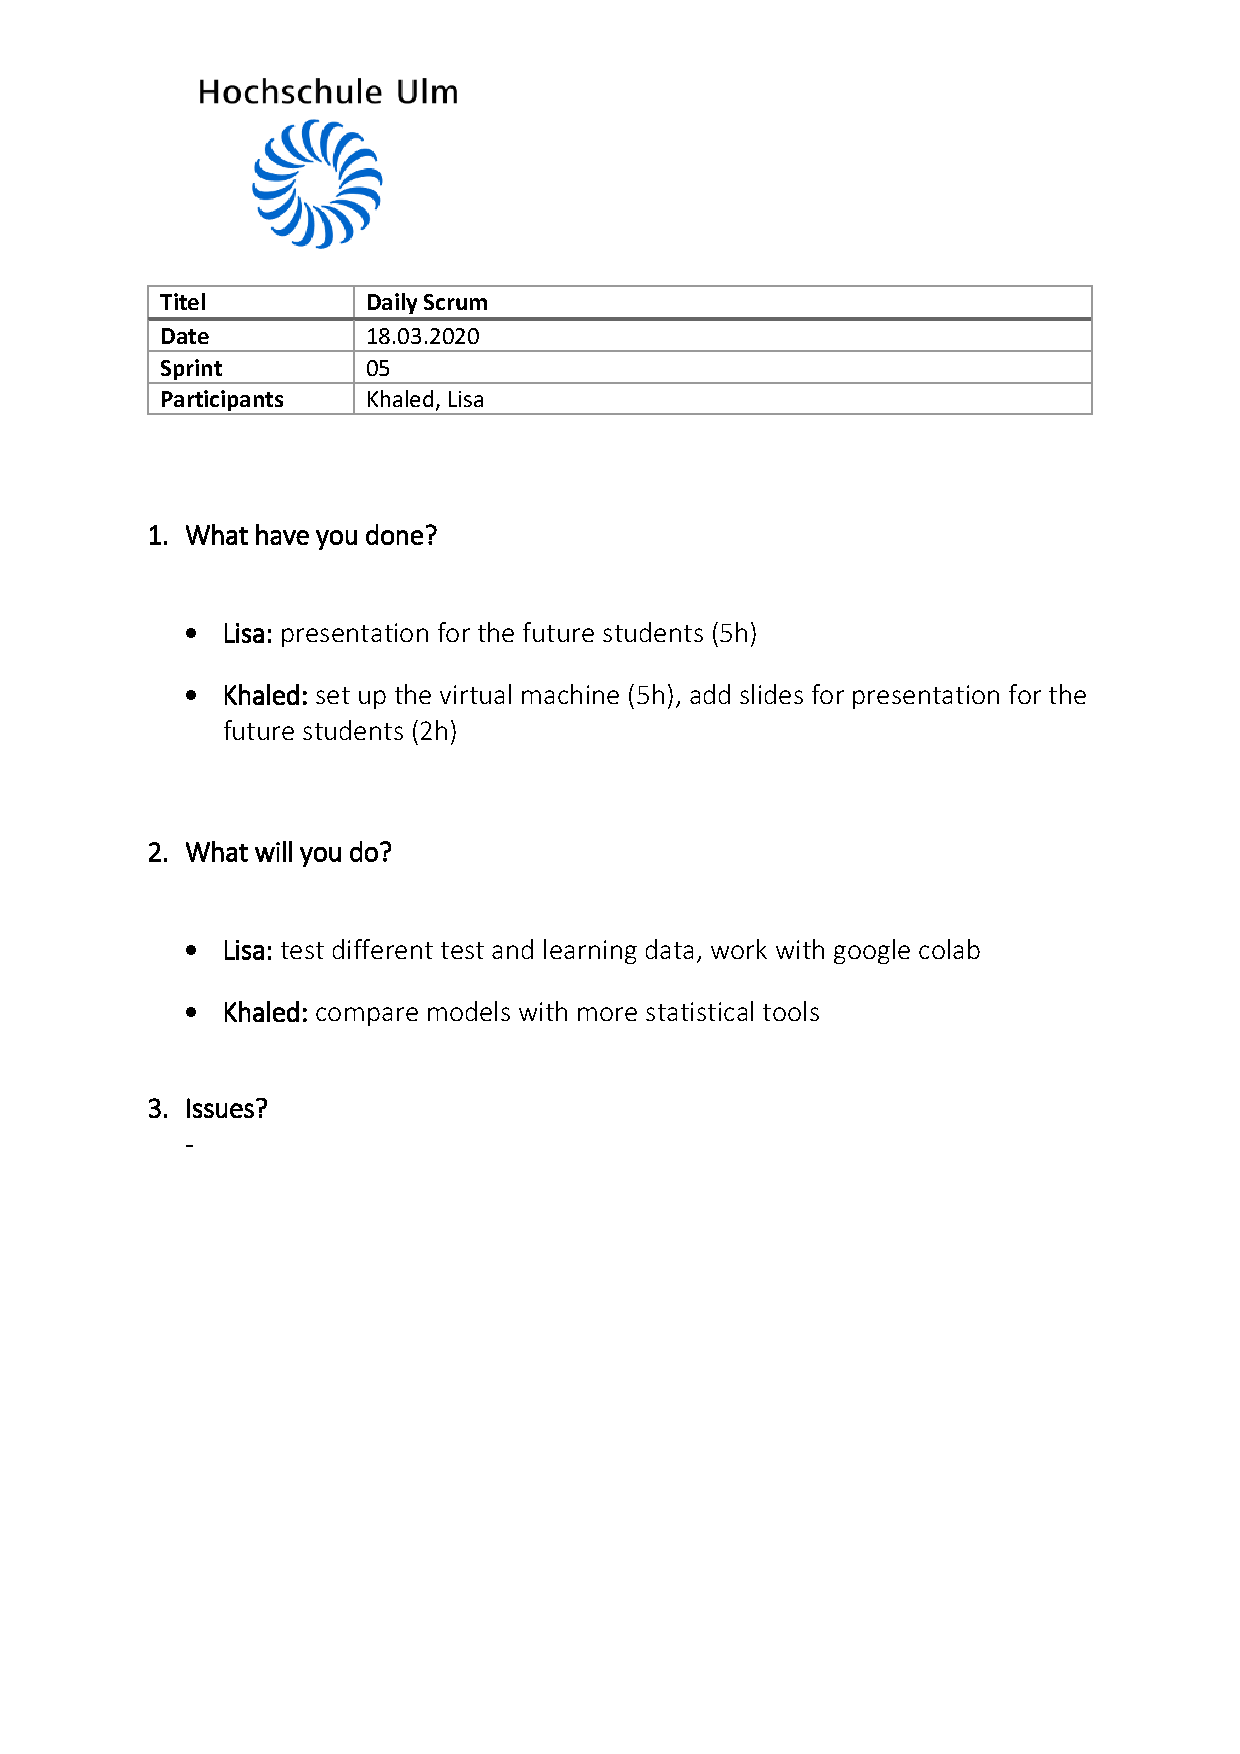
\includepdf[pages={1}]{pdf/Daily_Scrum_51.pdf}
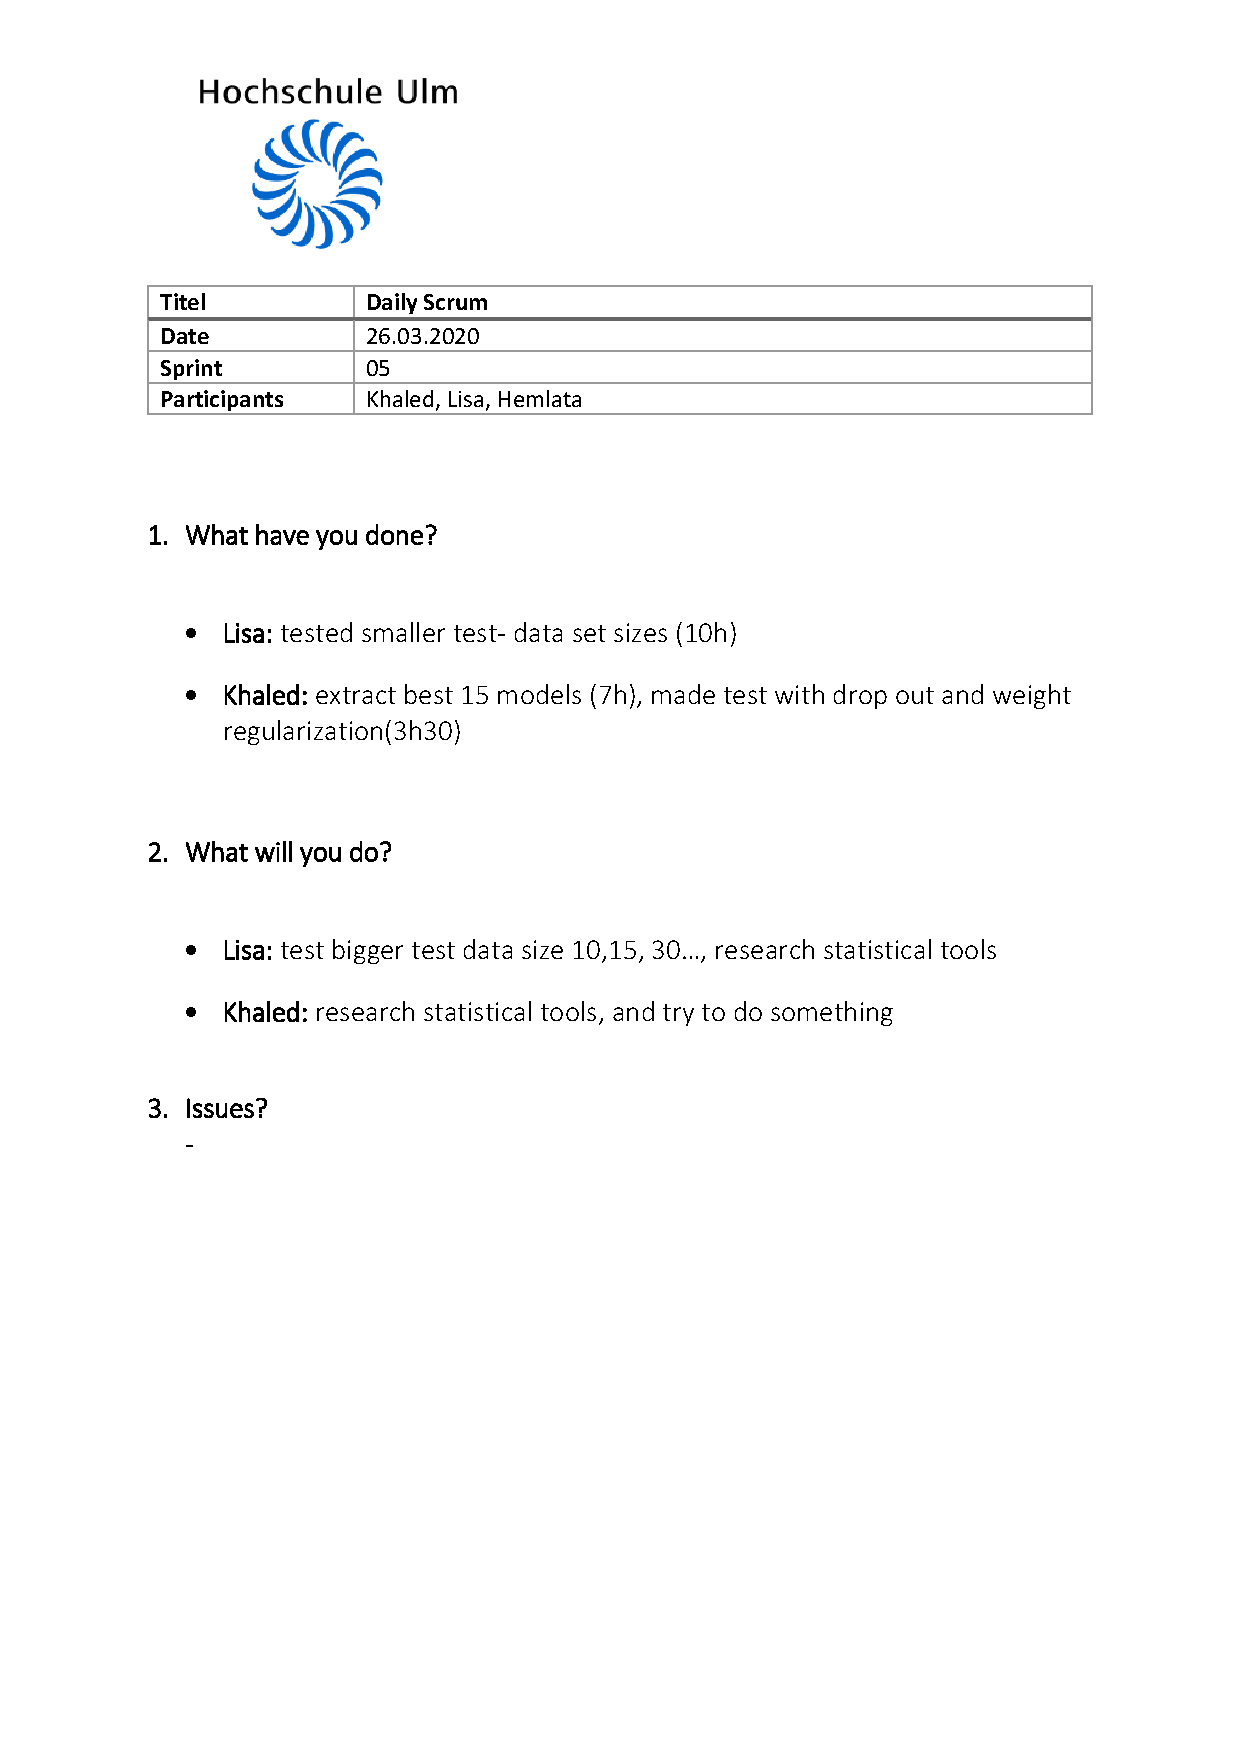
\includepdf[pages={1}]{pdf/Daily_Scrum_52.pdf}
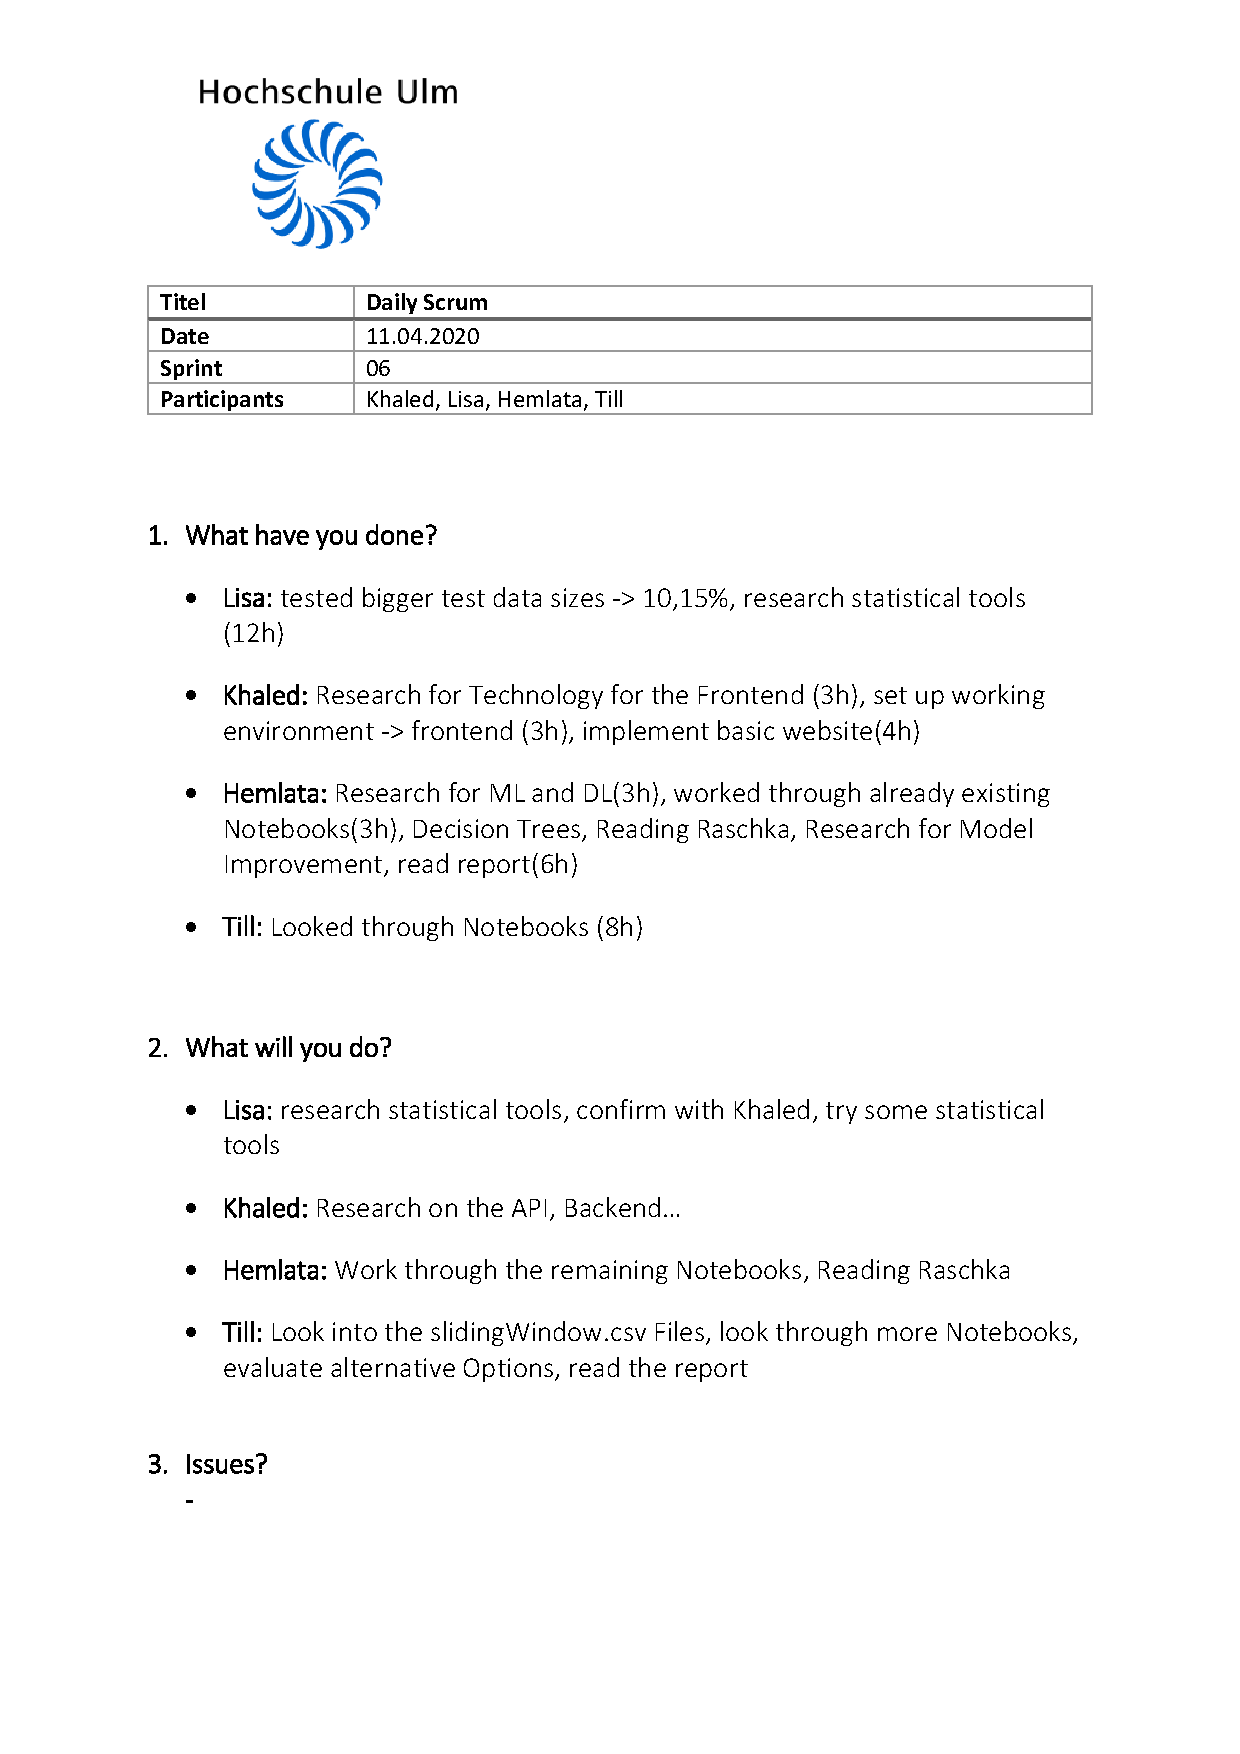
\includepdf[pages={1}]{pdf/Daily_Scrum_61.pdf}
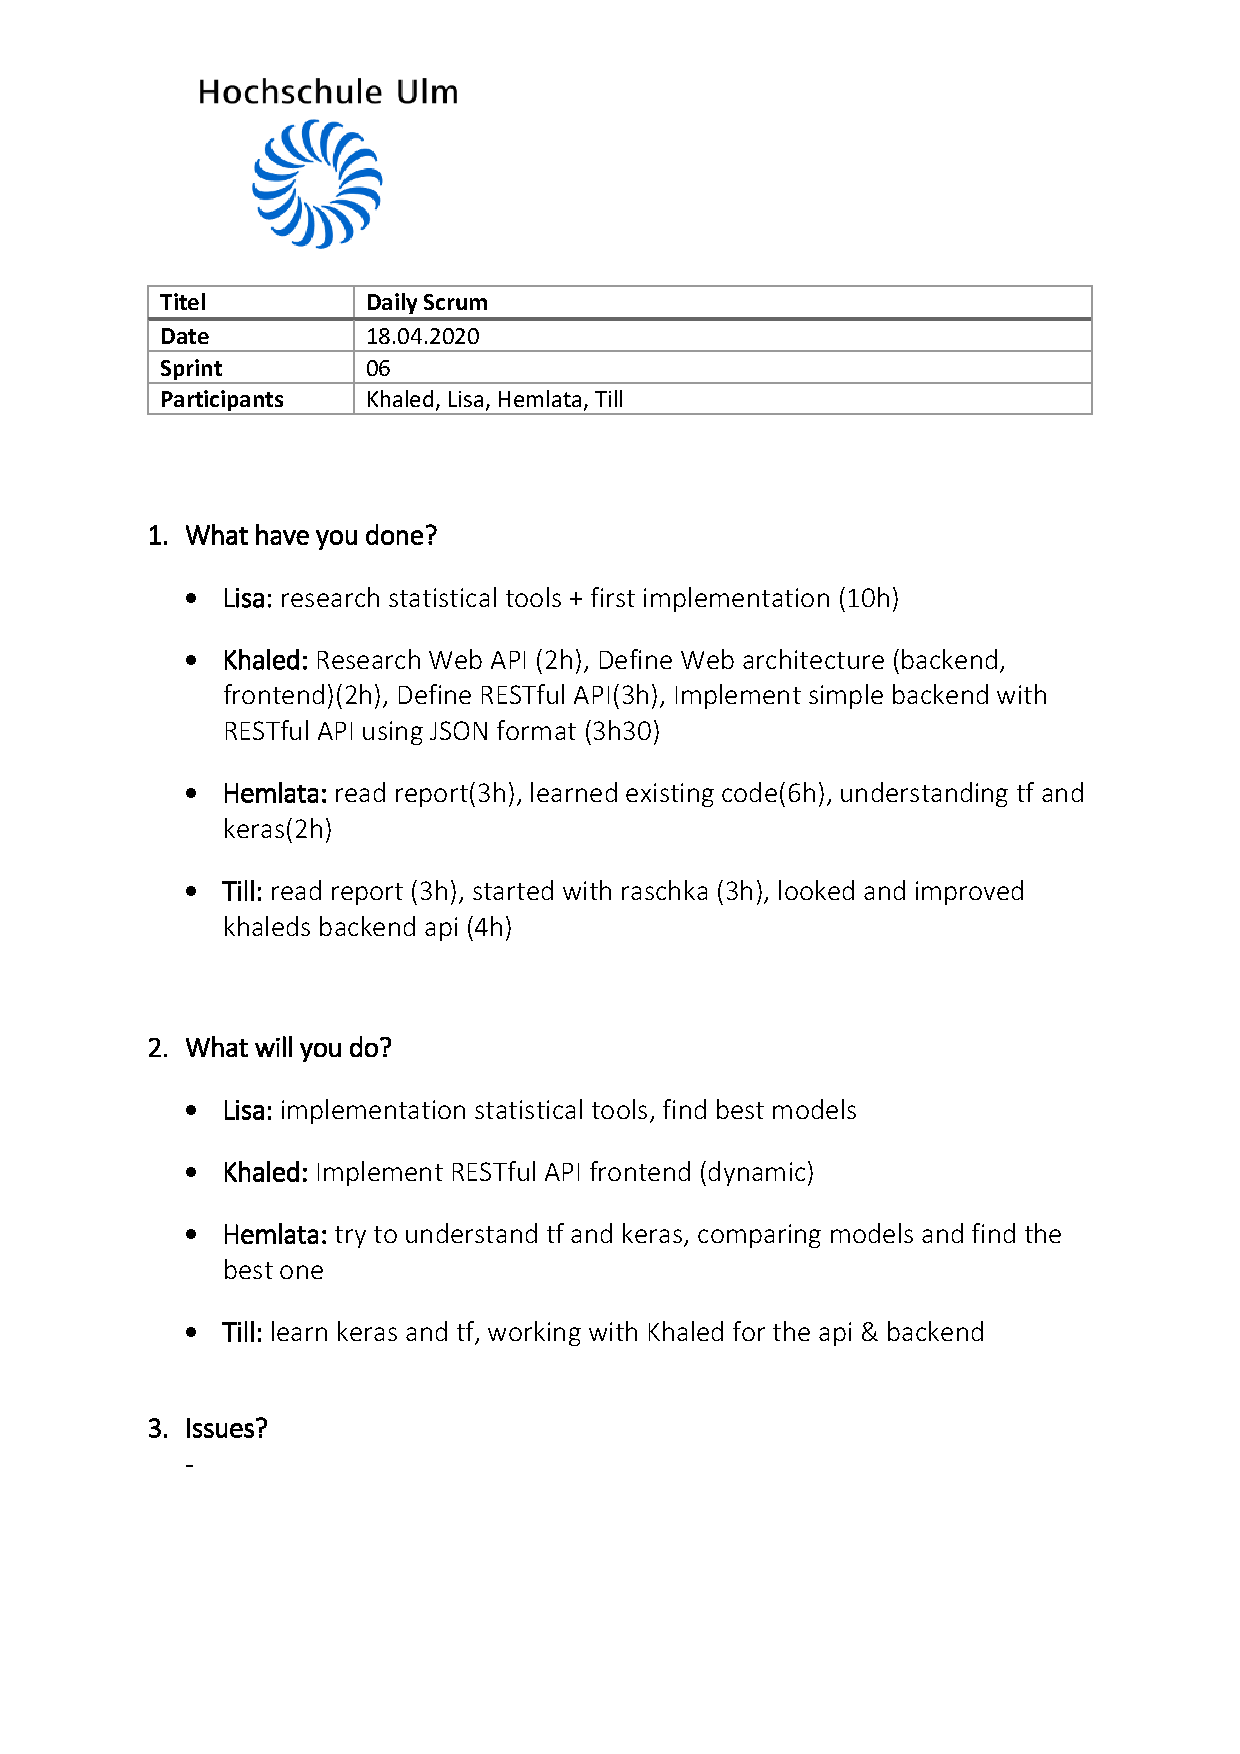
\includepdf[pages={1}]{pdf/Daily_Scrum_62.pdf}
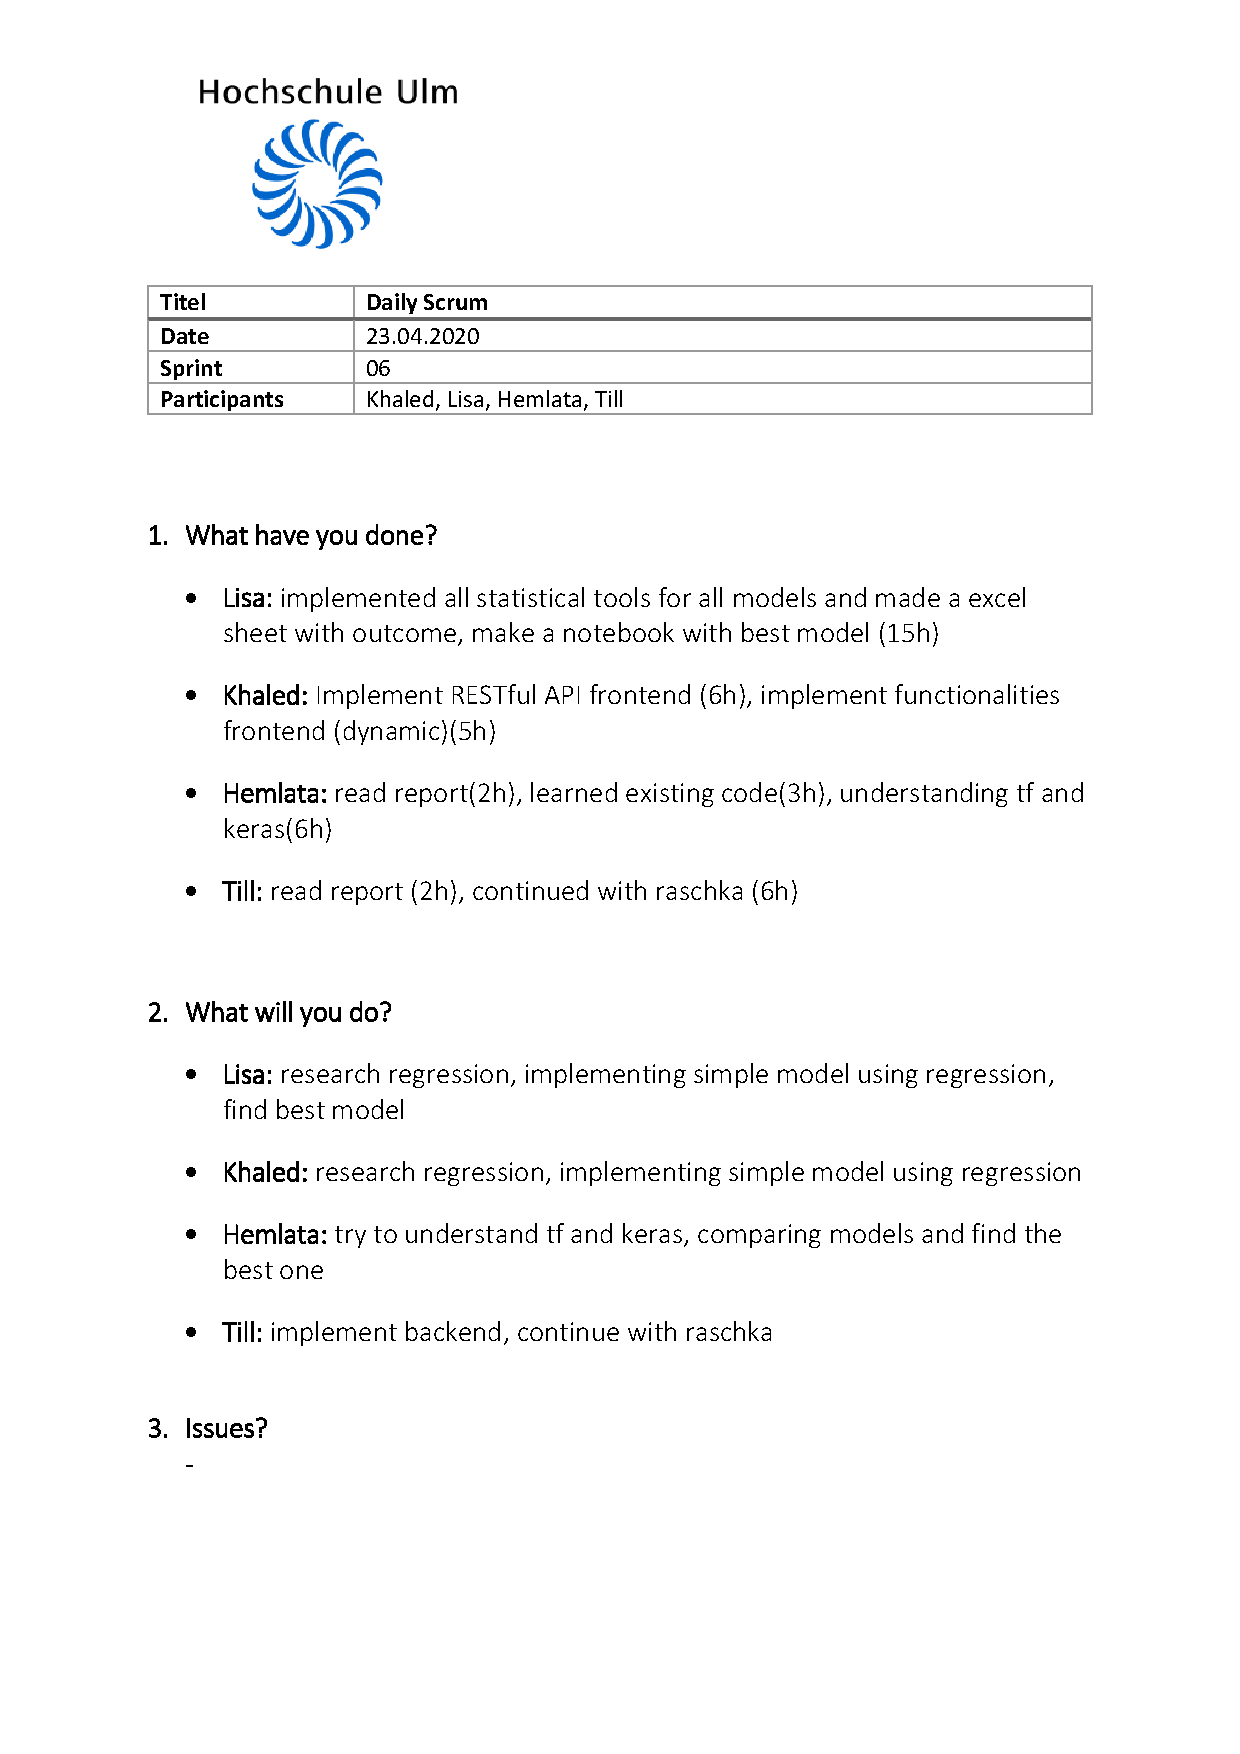
\includepdf[pages={1}]{pdf/Daily_Scrum_63.pdf}
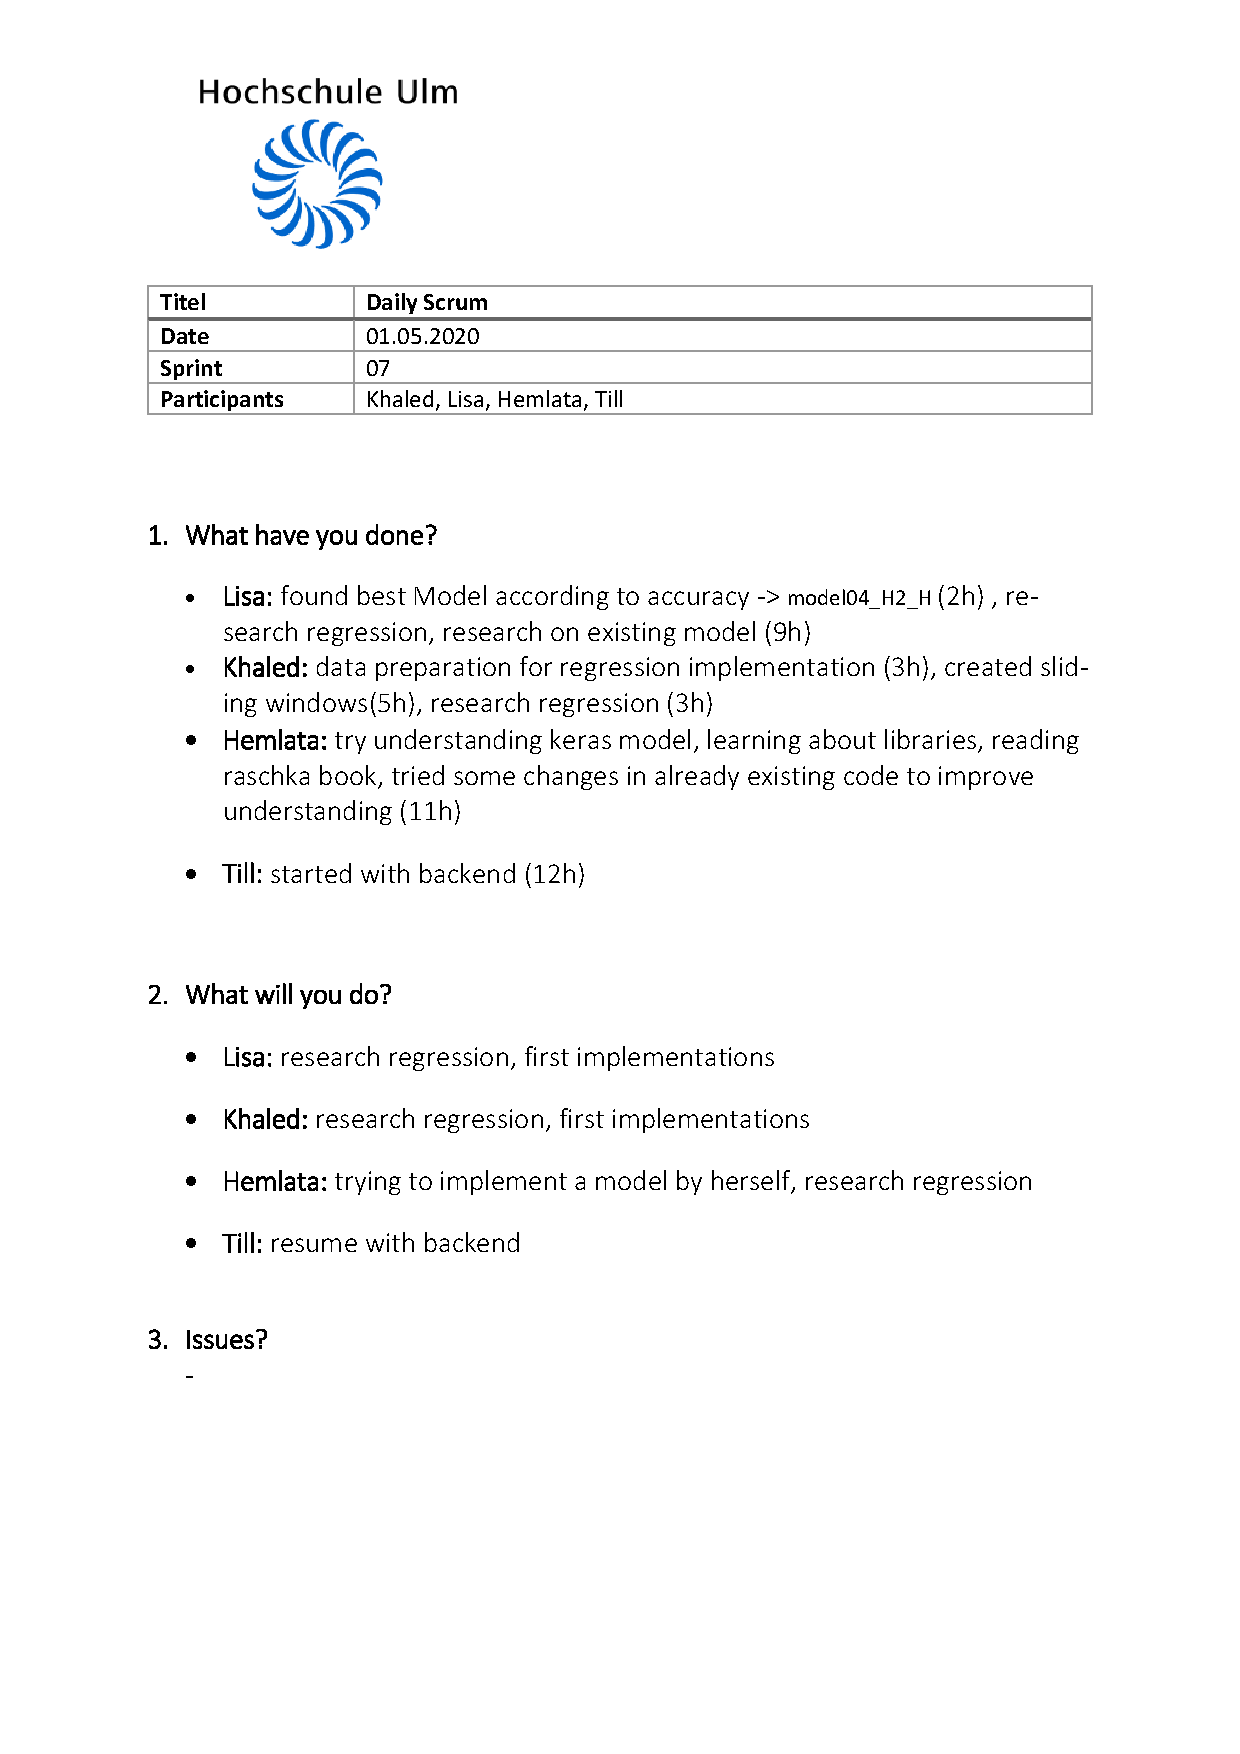
\includepdf[pages={1}]{pdf/Daily_Scrum_71.pdf}
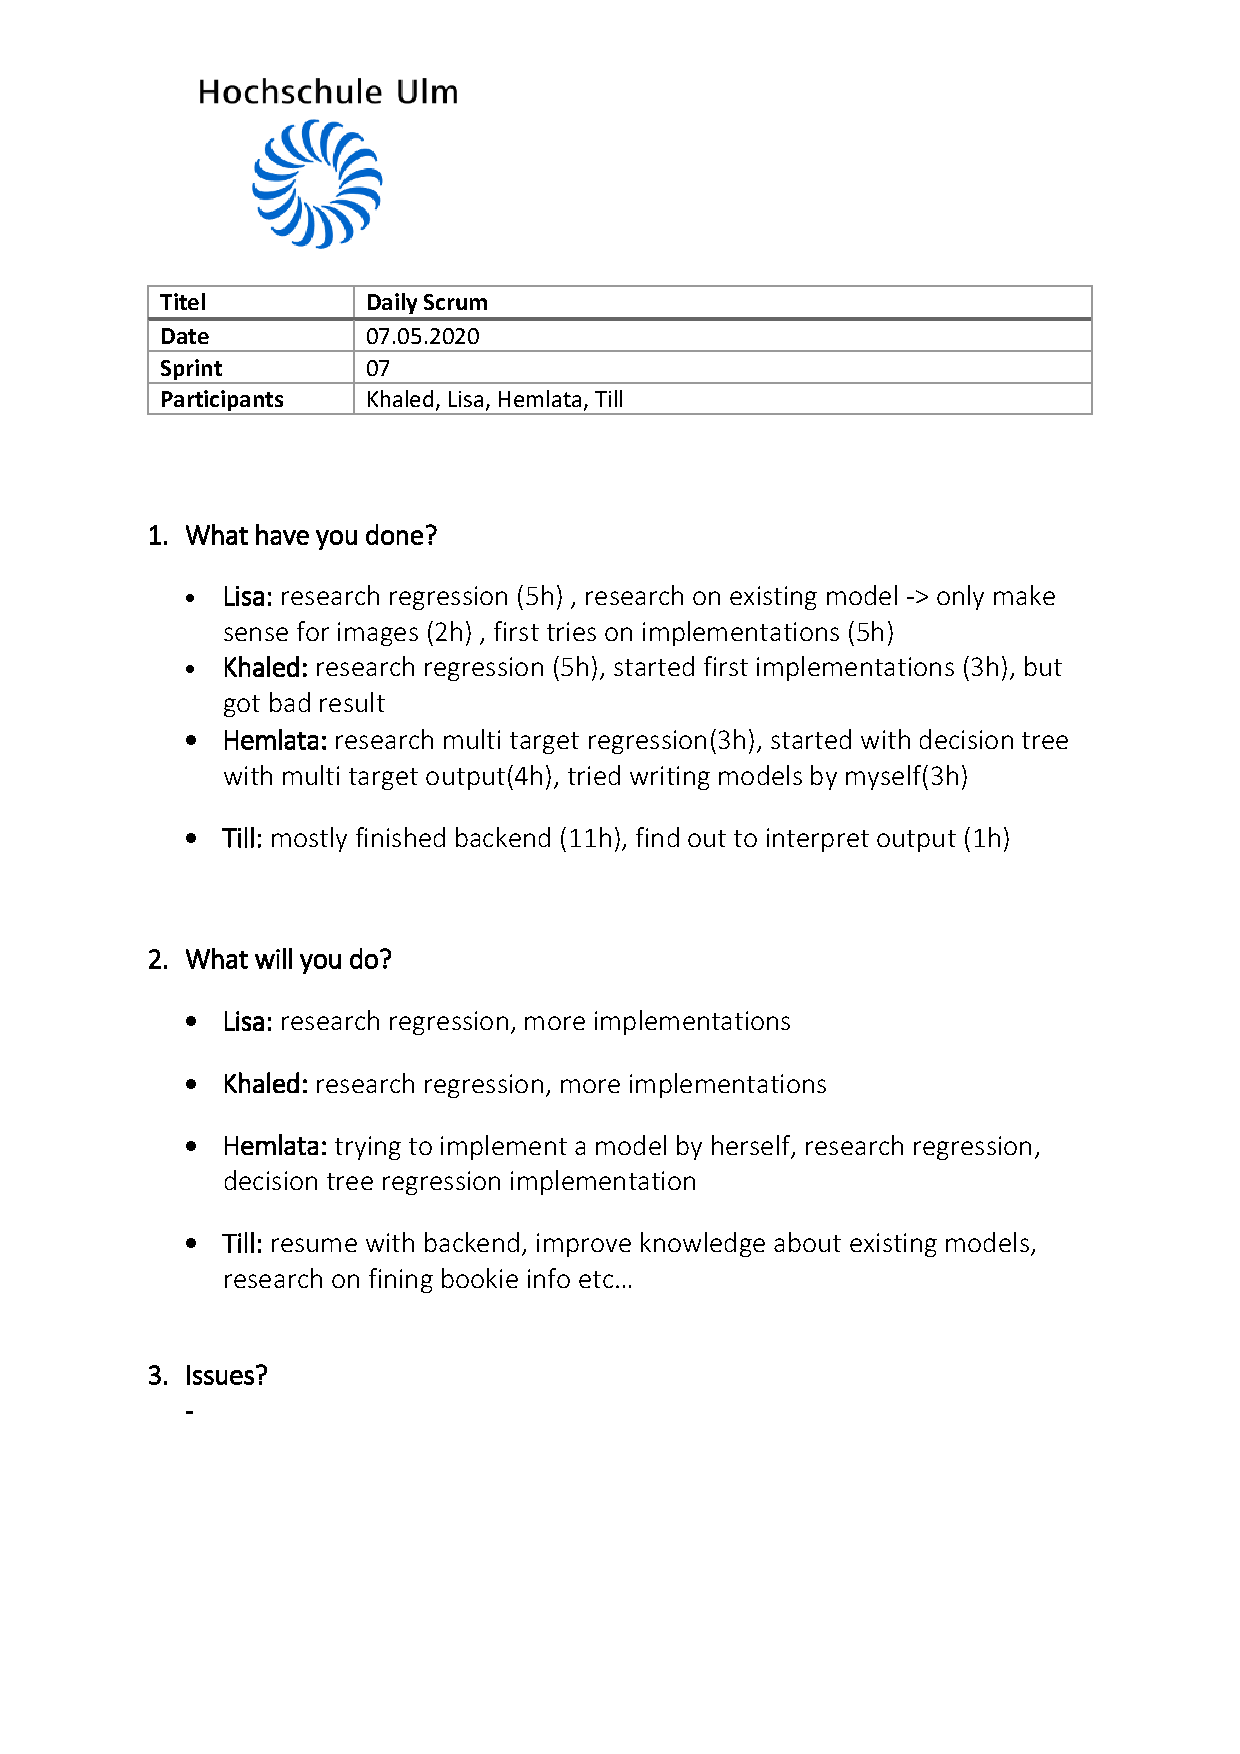
\includepdf[pages={1}]{pdf/Daily_Scrum_72.pdf}
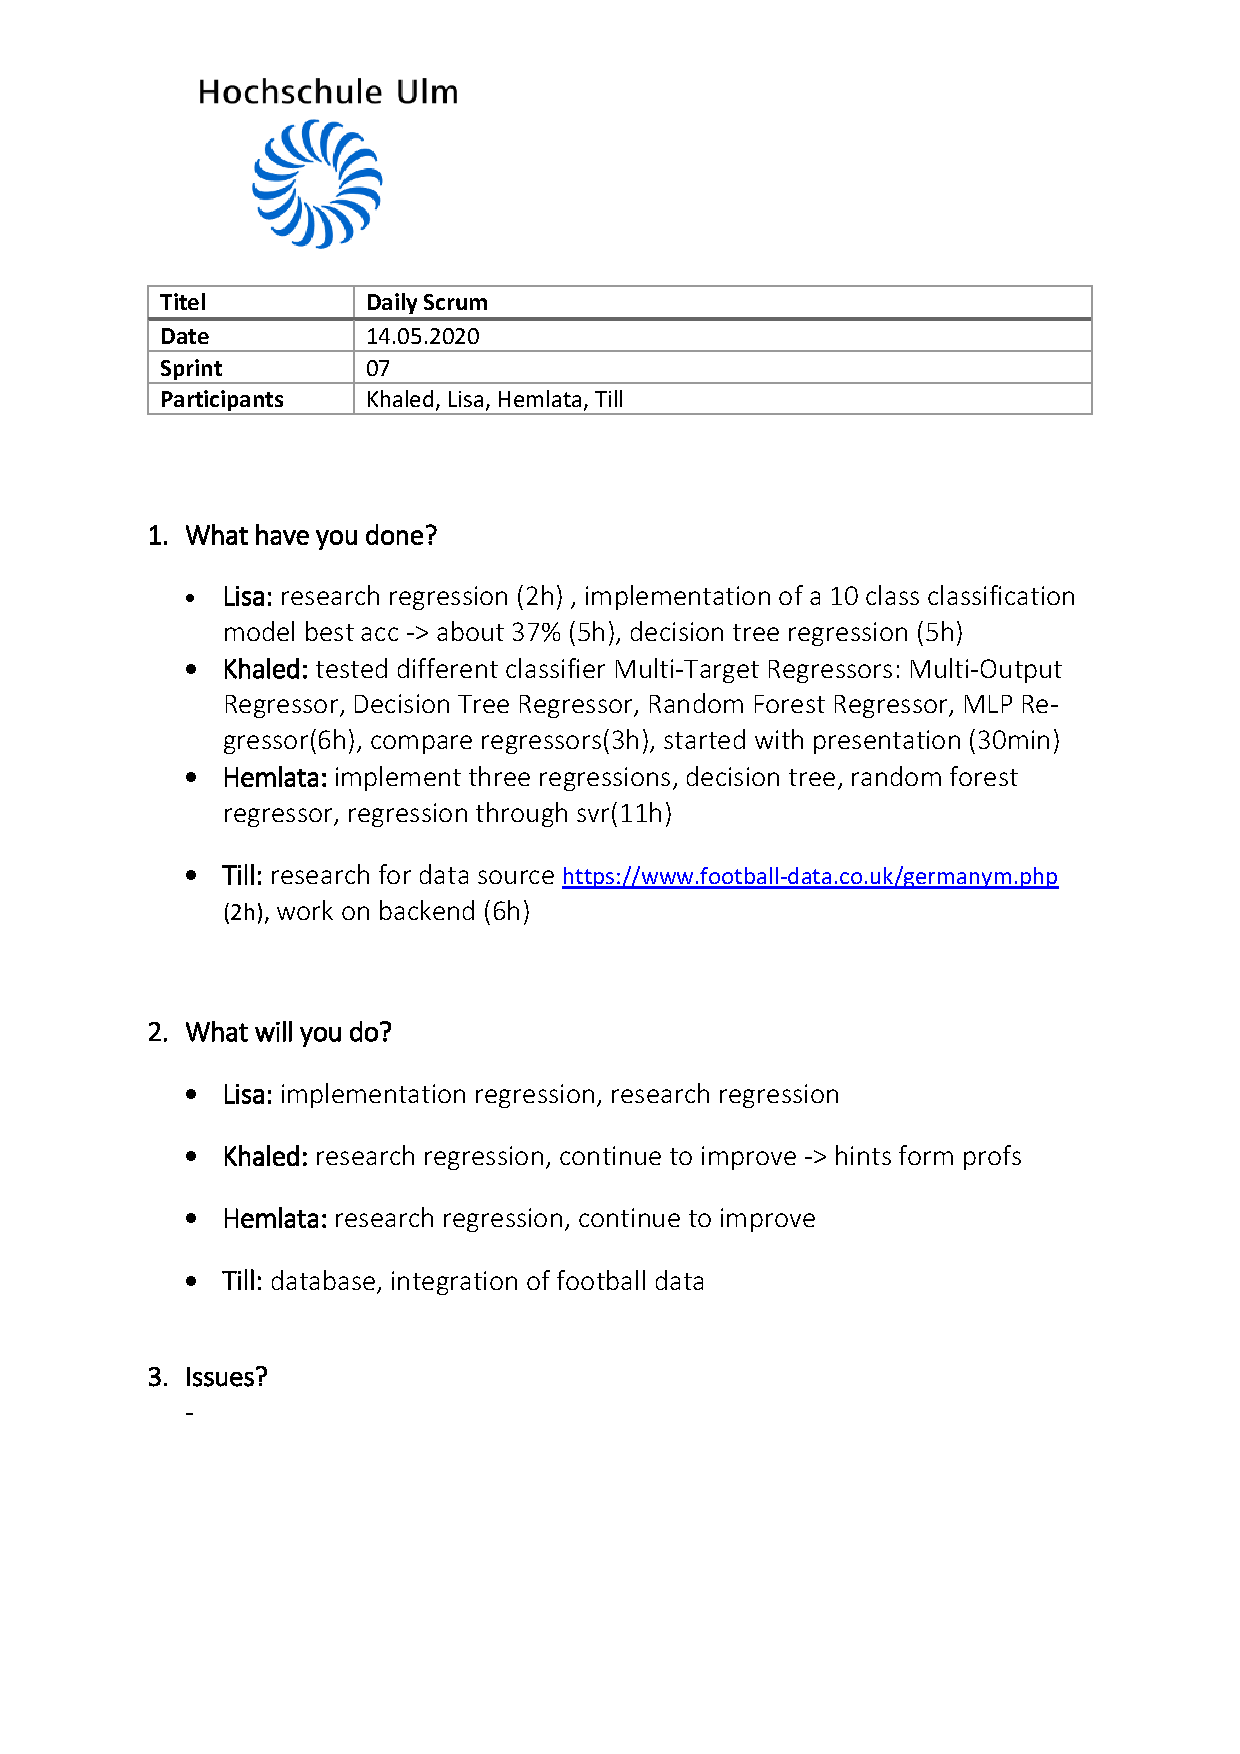
\includepdf[pages={1}]{pdf/Daily_Scrum_73.pdf}
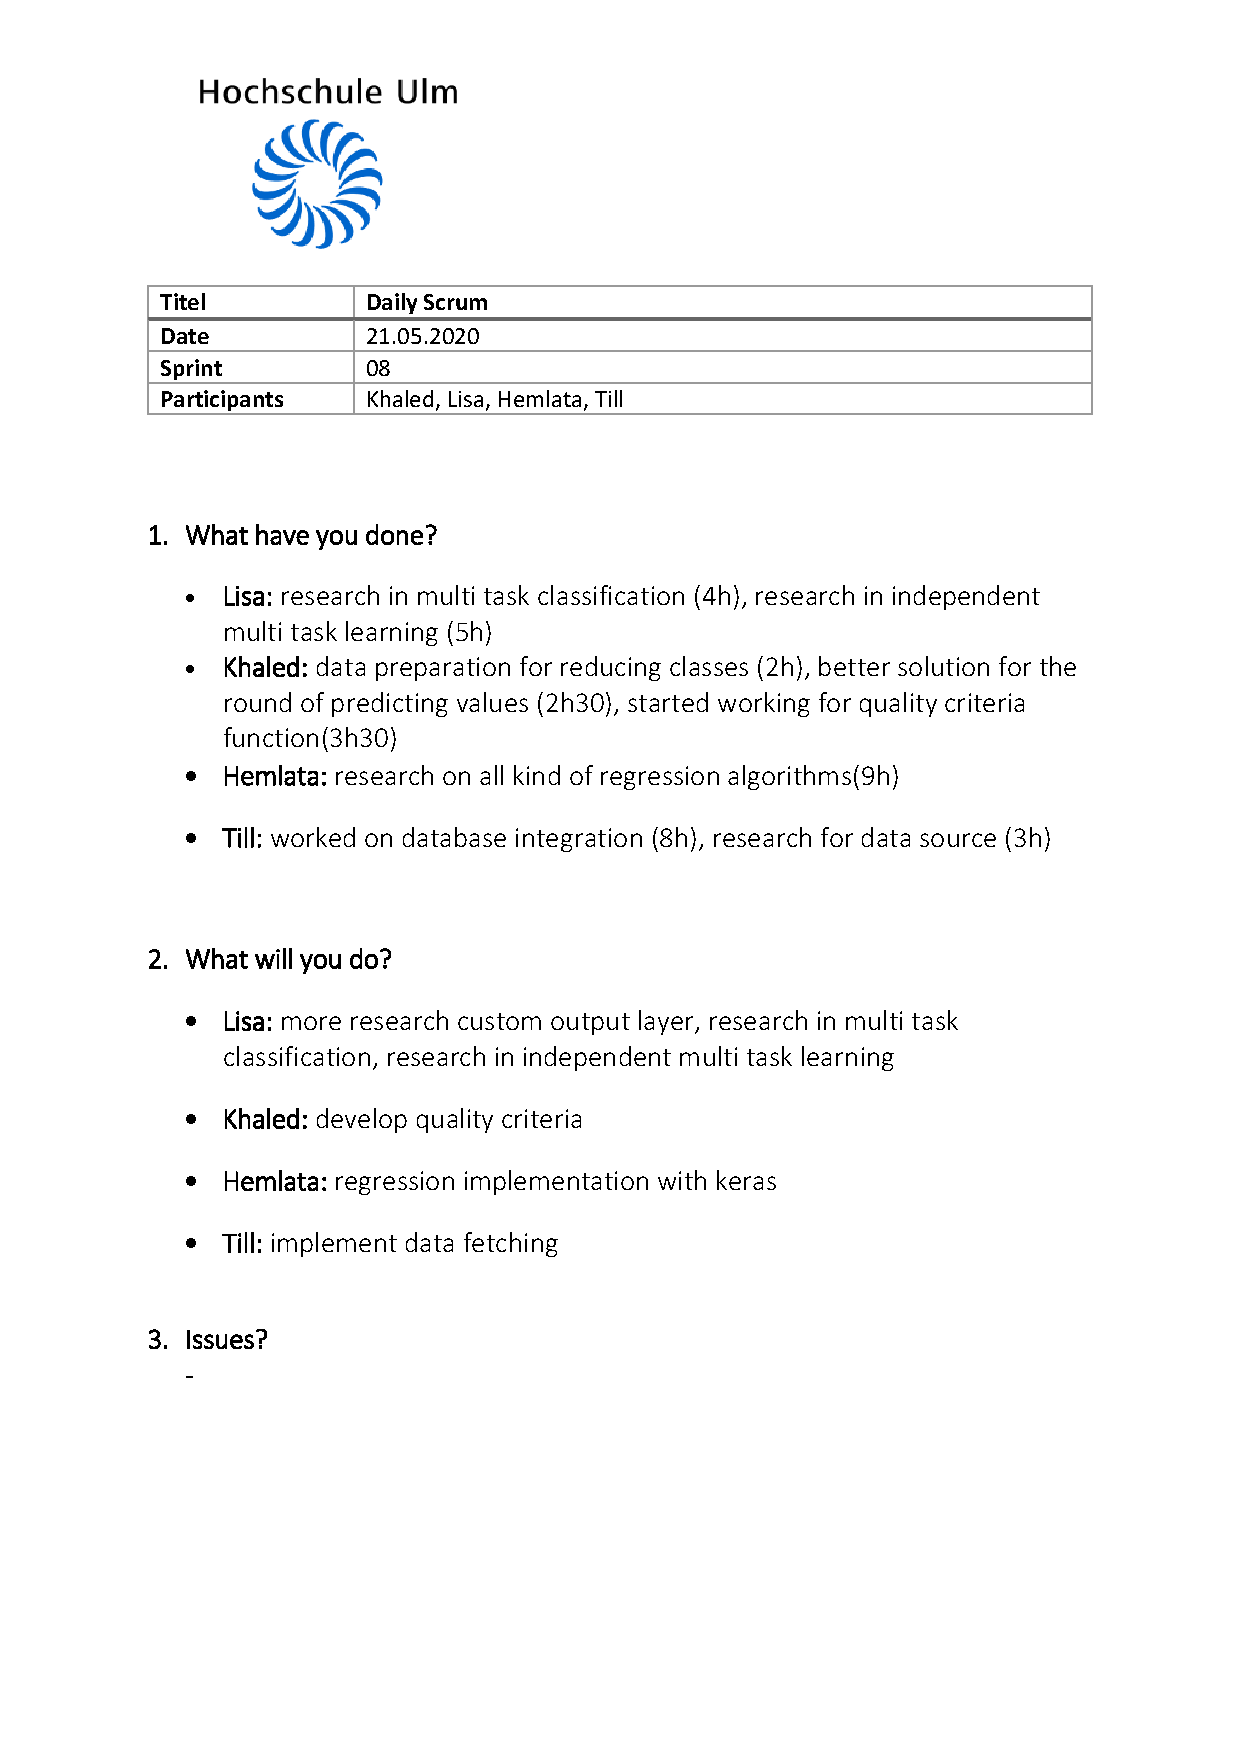
\includepdf[pages={1}]{pdf/Daily_Scrum_81.pdf}
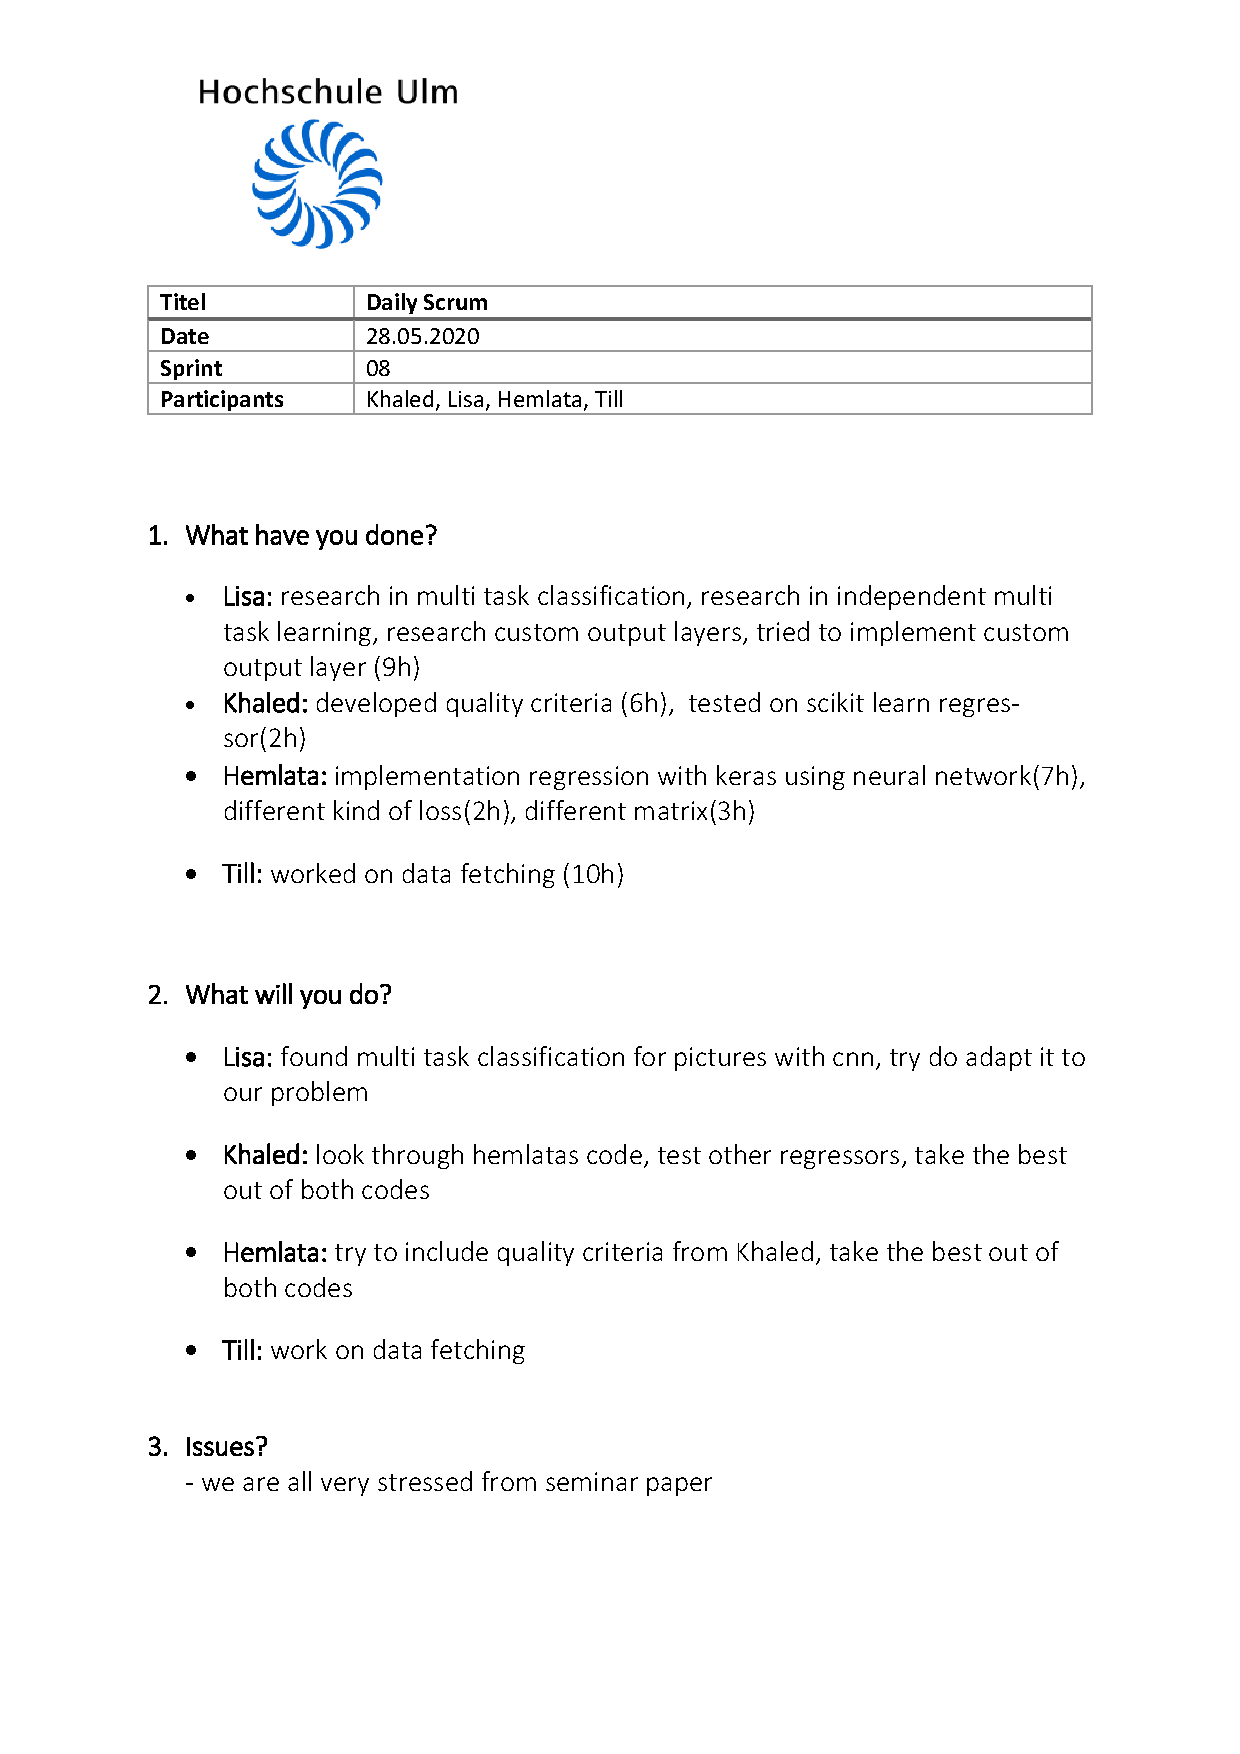
\includepdf[pages={1}]{pdf/Daily_Scrum_82.pdf}
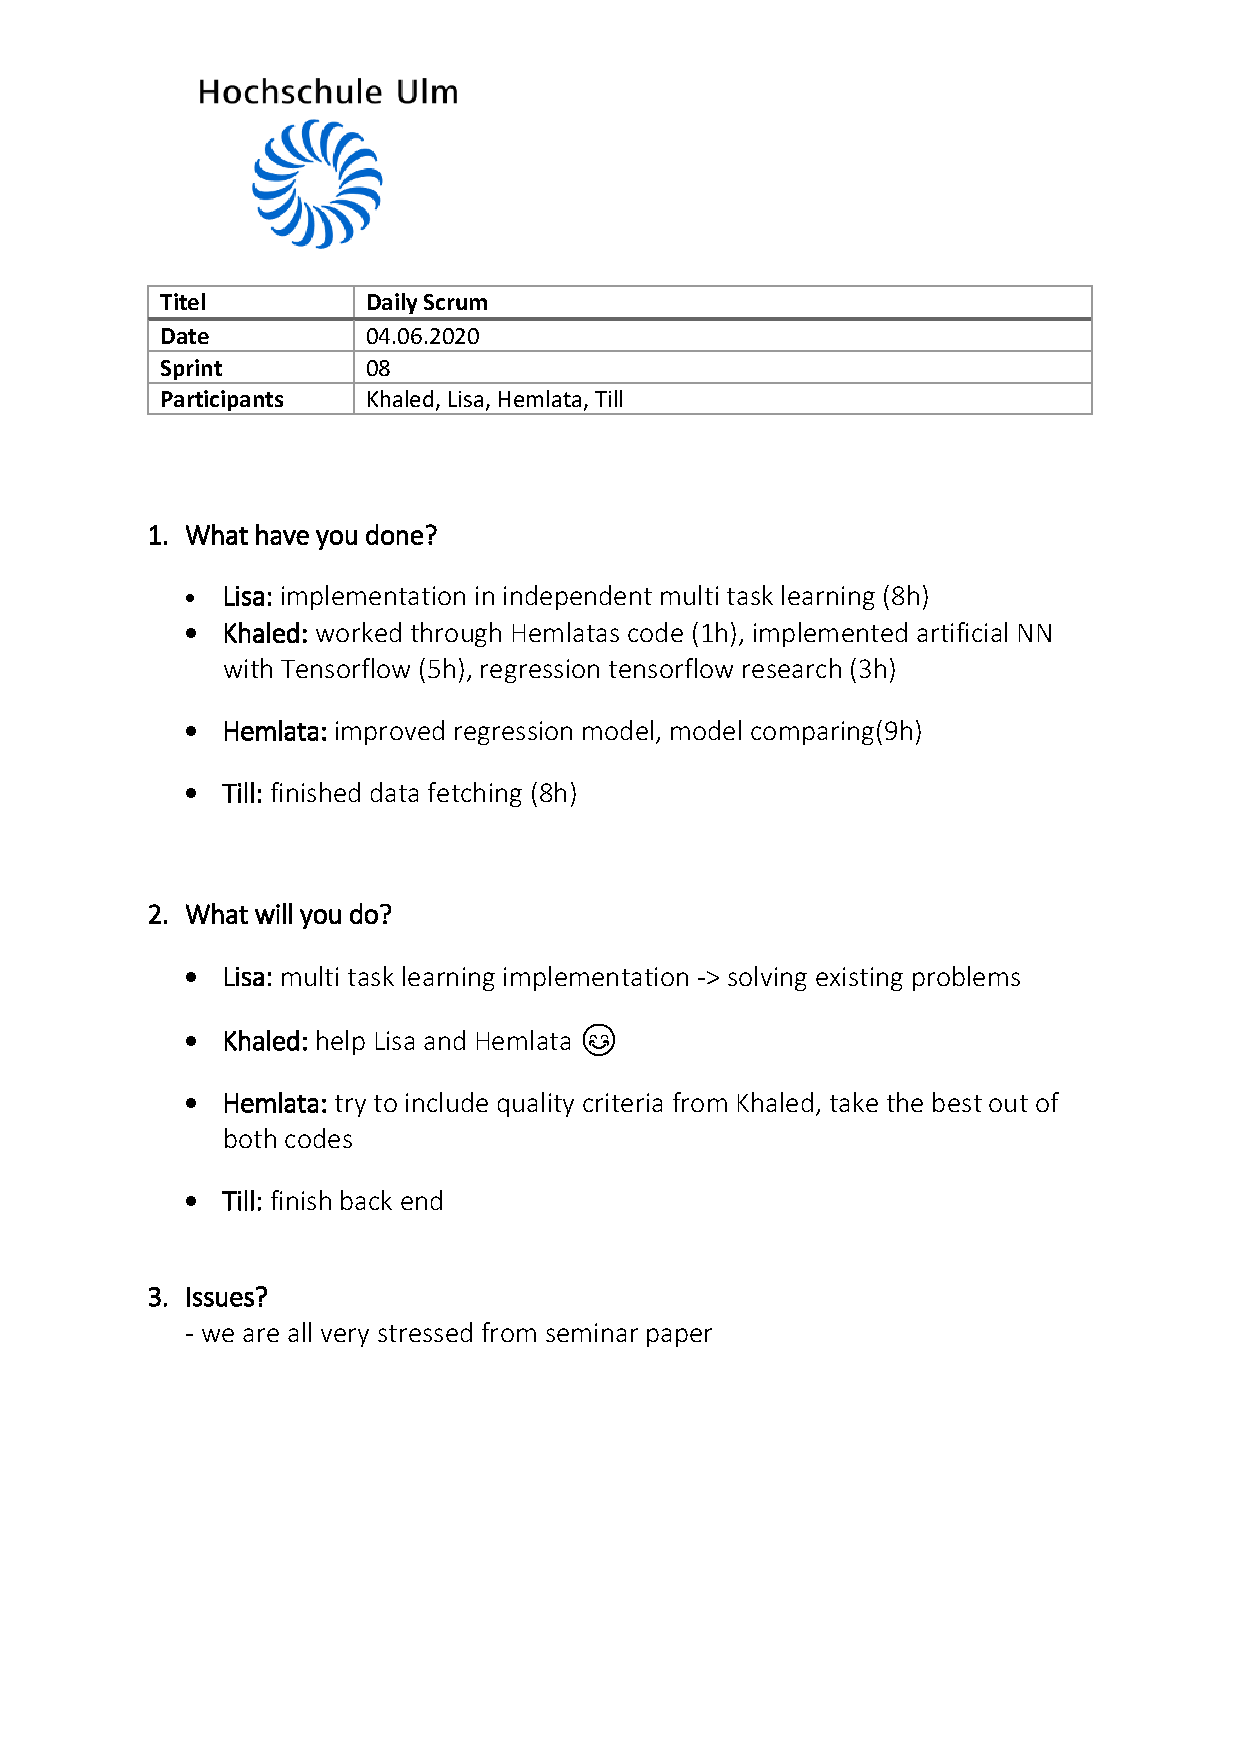
\includepdf[pages={1}]{pdf/Daily_Scrum_83.pdf}
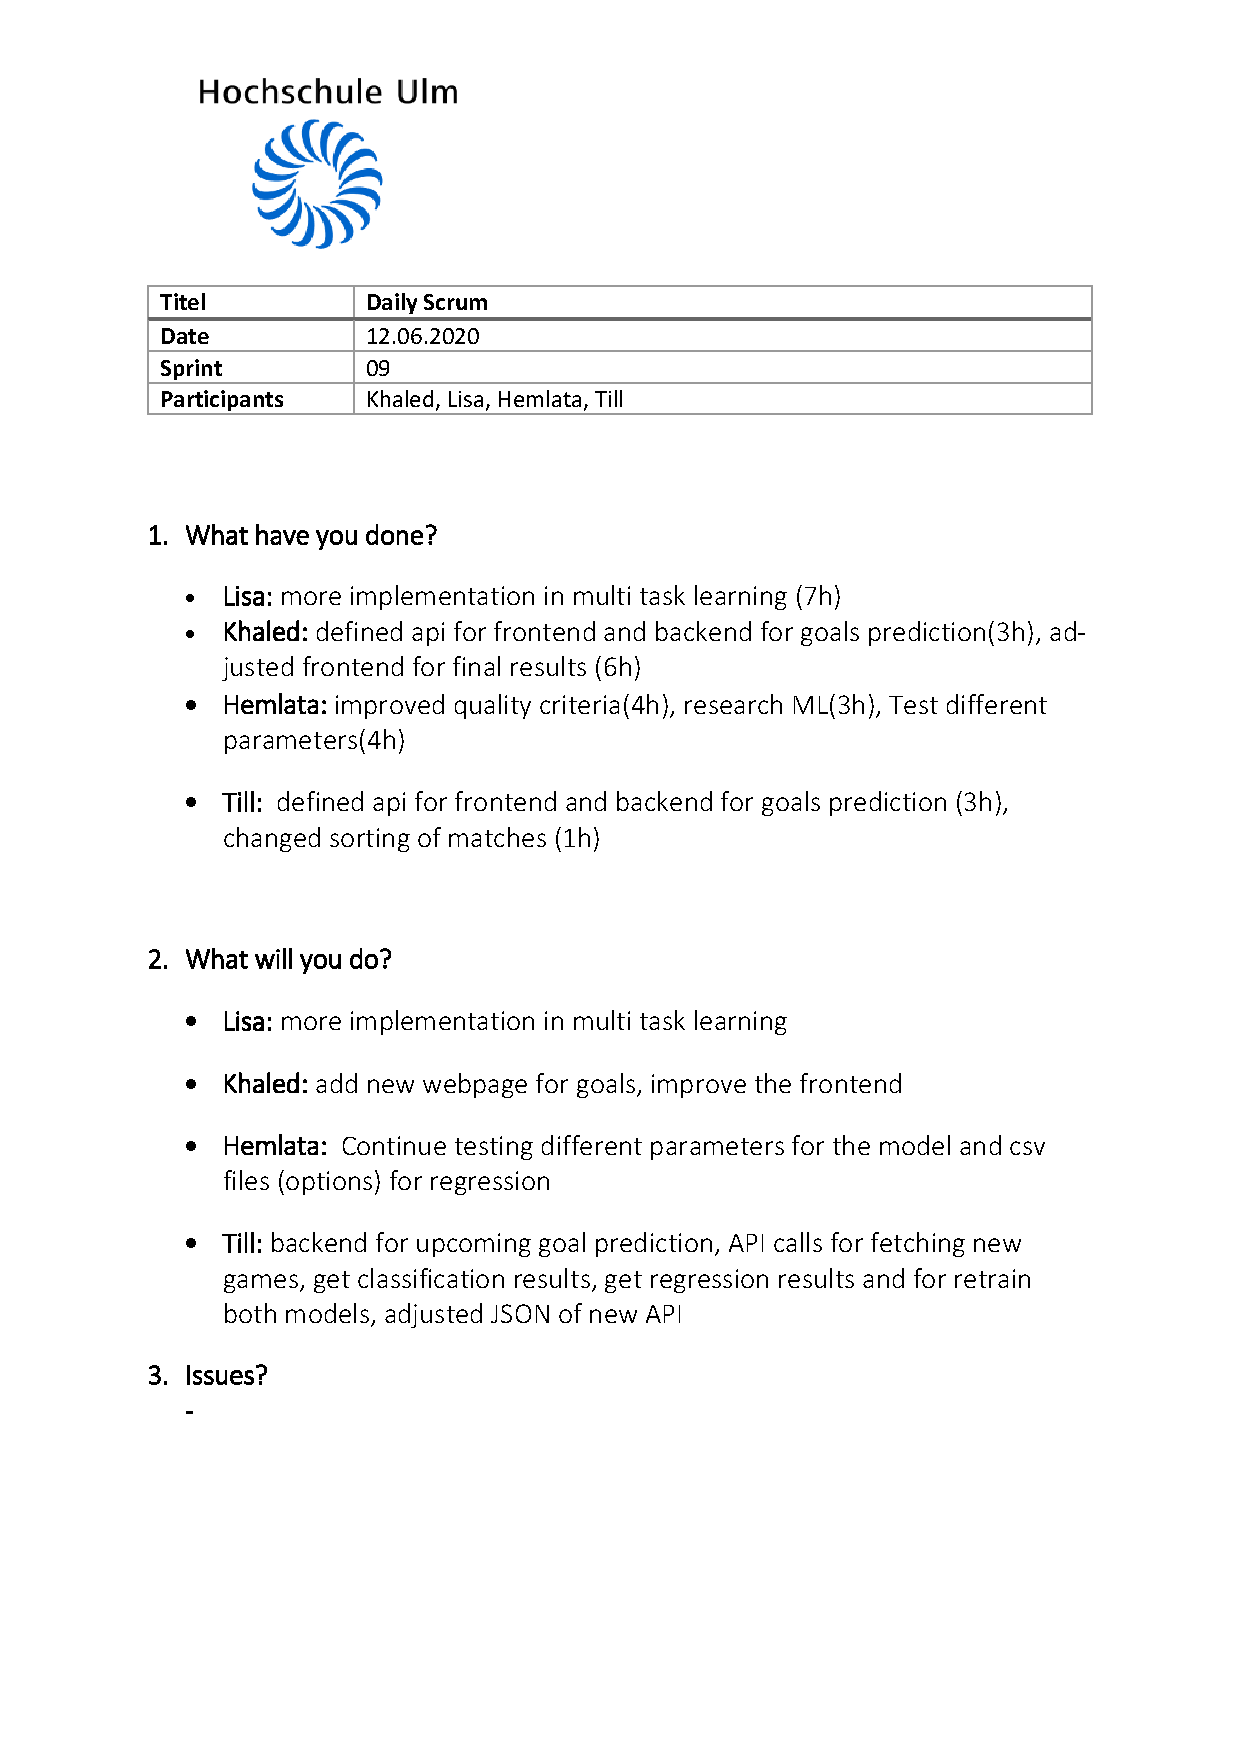
\includepdf[pages={1}]{pdf/Daily_Scrum_91.pdf}
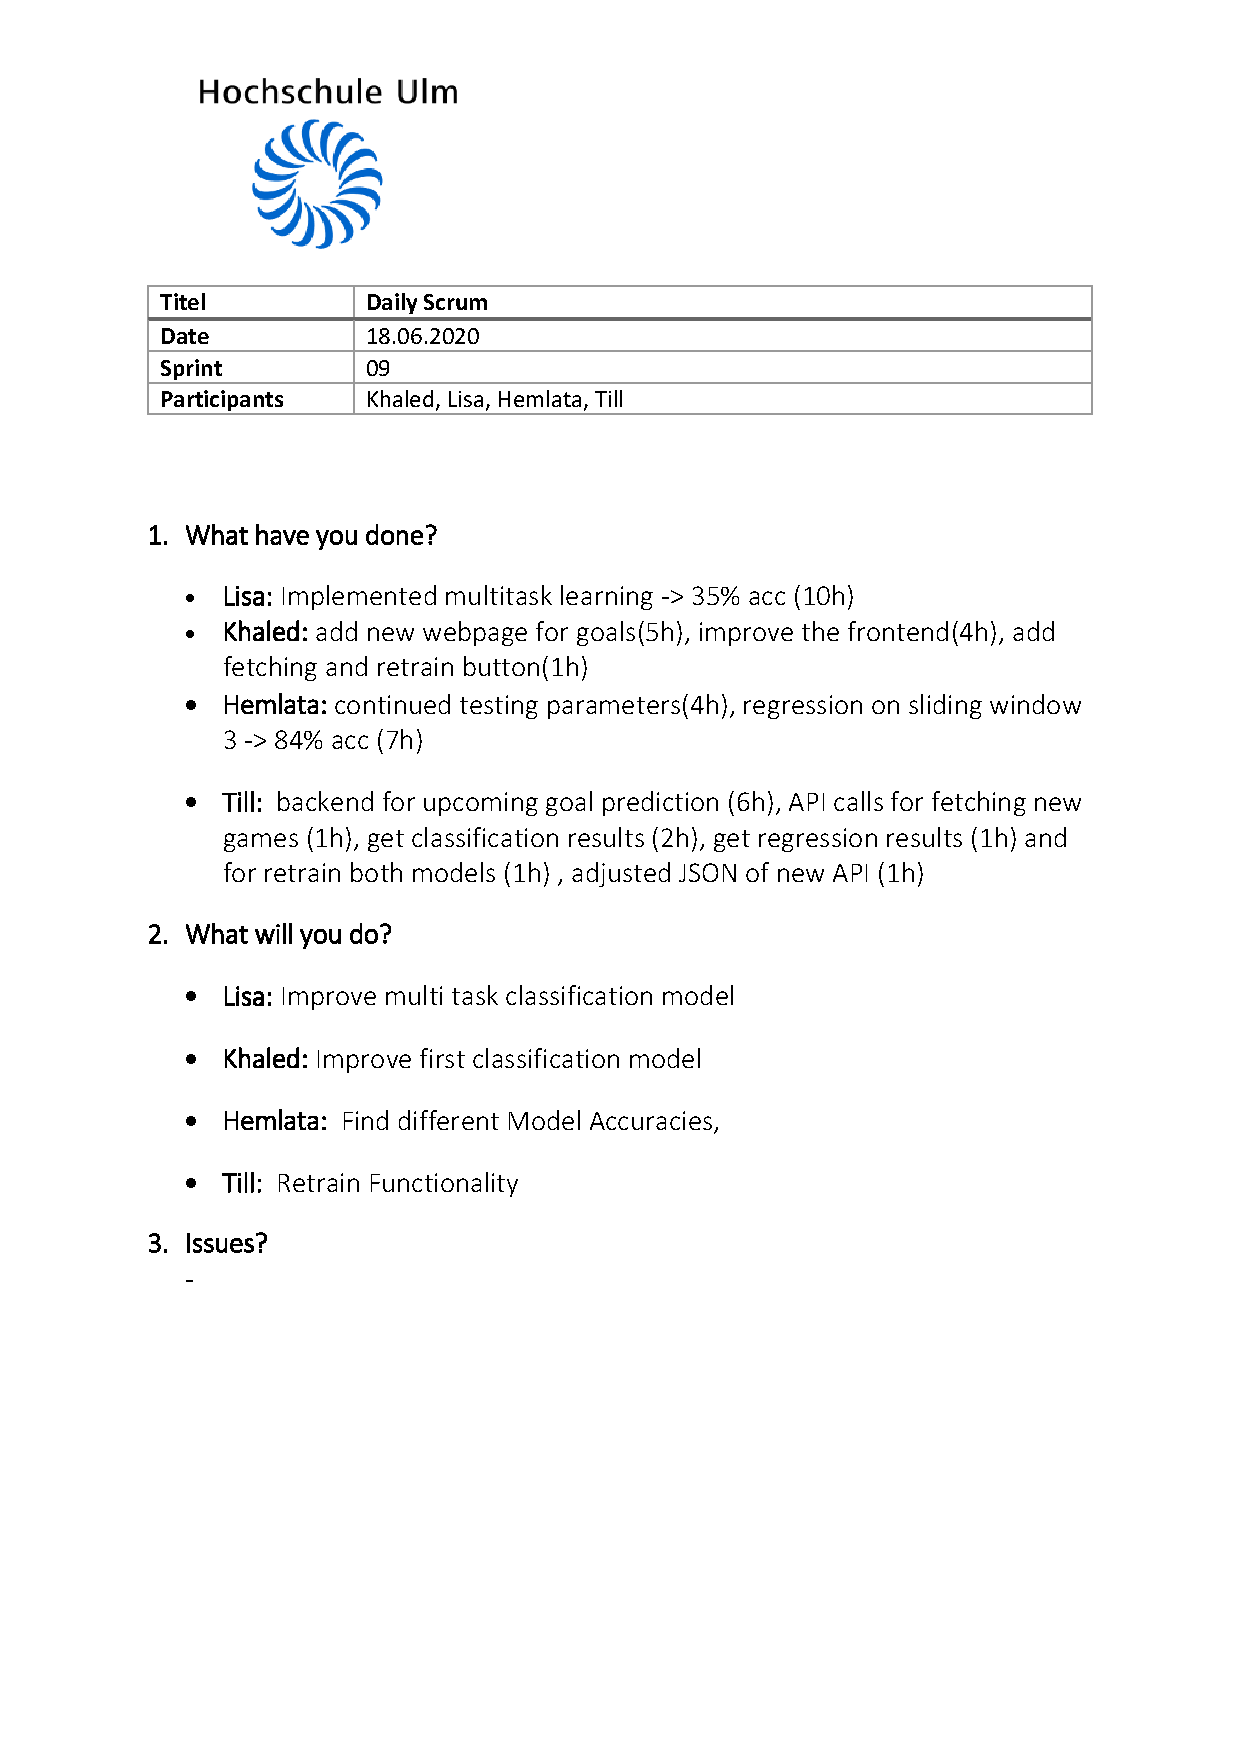
\includepdf[pages={1}]{pdf/Daily_Scrum_92.pdf}
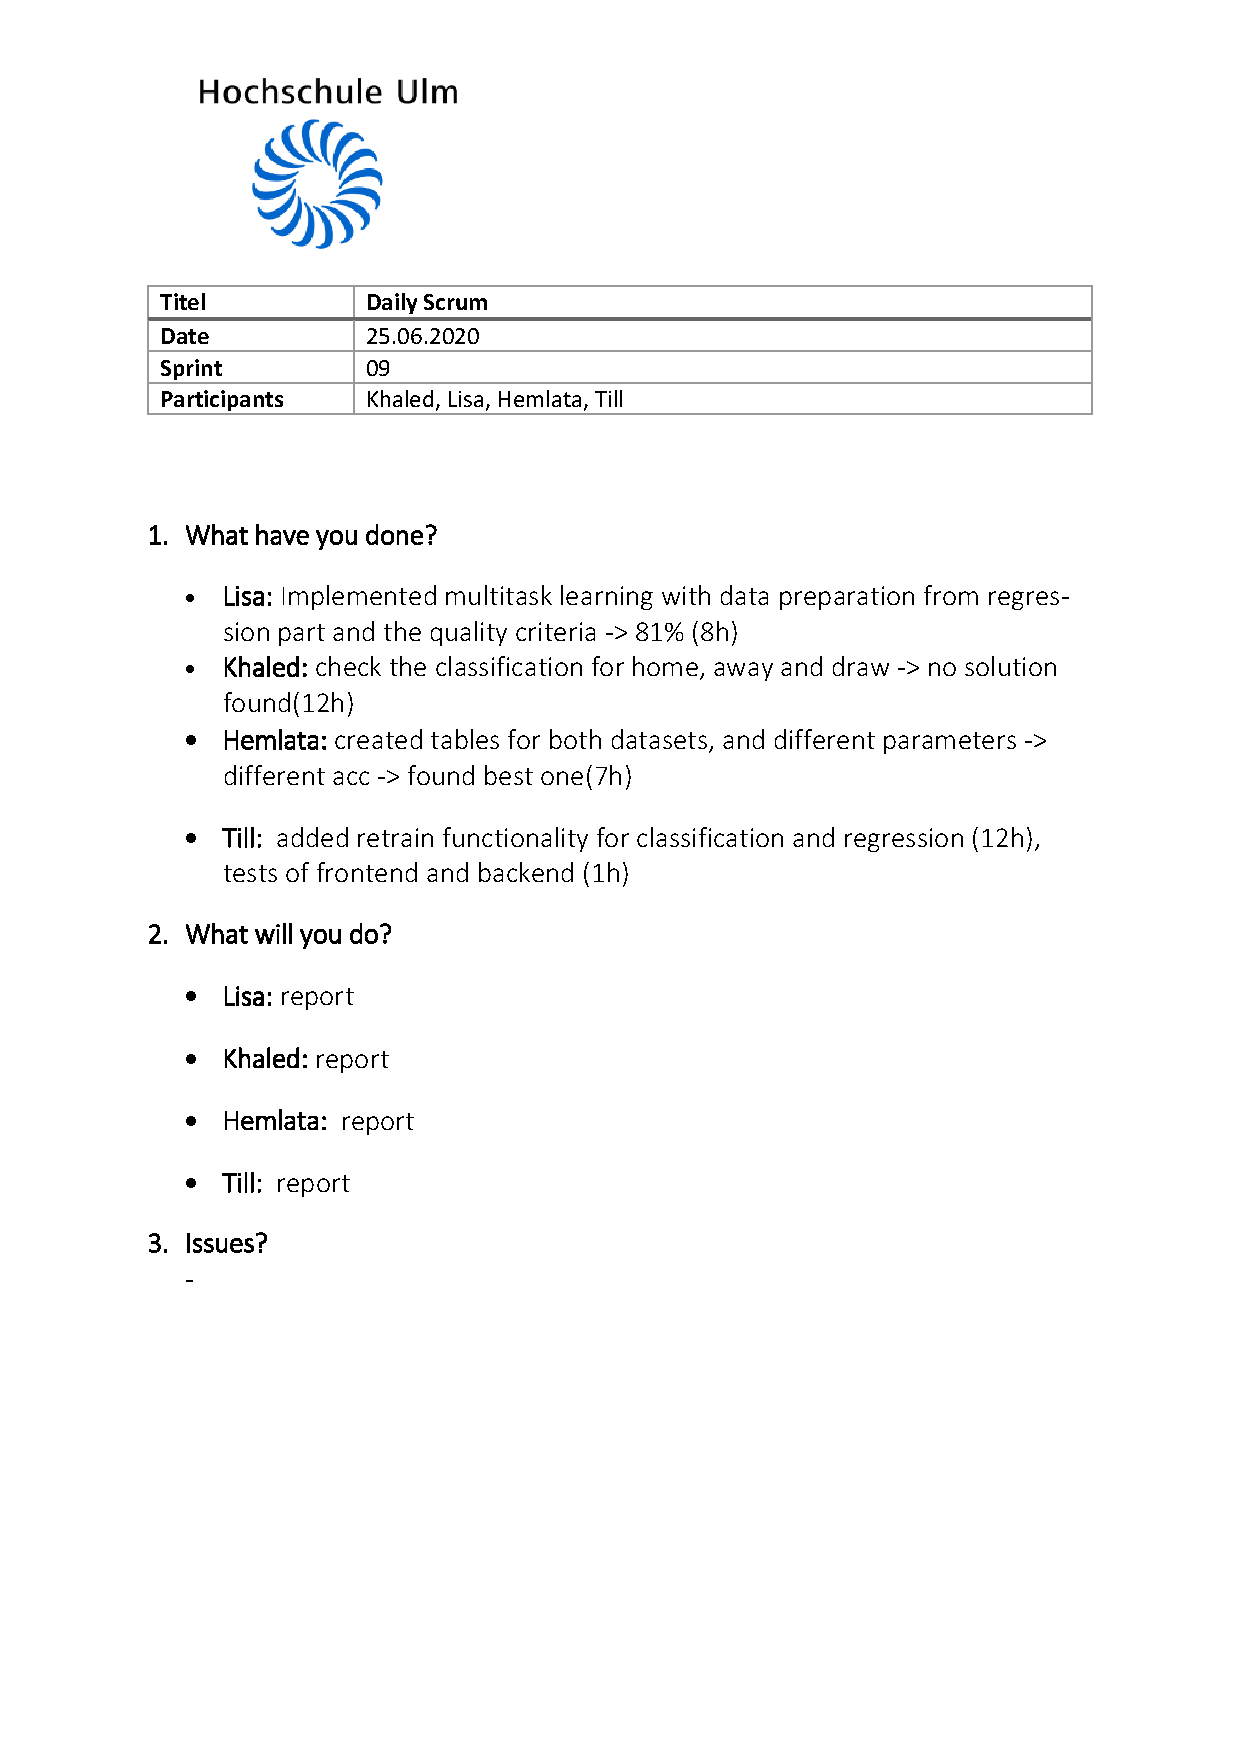
\includepdf[pages={1}]{pdf/Daily_Scrum_93.pdf}

%\newpage
%\section{ Report of First Semester}
%\label{section:appendix_c}
%\newpage

	
\end{document}
 

% Include document settings
%!TEX root = ../main.tex

%% Document language (en, de)
\newcommand{\documentLanguage}{en}

%% Document type
% T2\_1000 Project Thesis (Semester 1 & 2)
% T2\_2000 Project Thesis (Semester 3 & 4)
% T2\_3100 Seminar Paper (Semester 5 & 6)
% T2\_3300 Bachelor Thesis
\newcommand{\documentType}{T2\_3300}

\newcommand{\documentAuthor}{Lisa Boos, Hemlata Prajapati, Khaled Jallouli, Till Hoffmann}

\newcommand{\documentTitle}{Predicting the Outcome of Soccer Matches}

\newcommand{\documentPeriod}{6 months}

\newcommand{\matriculationNumber}{3133068}

\newcommand{\locationUniversity}{Ulm}
\newcommand{\department}{Informationssysteme}
\newcommand{\course}{}

\newcommand{\degree}{Master of Science}
% INF2014 - INF2016 (MI):         Bachelor of Science
% INF2014 - INF2016 (IA/IM) :   Bachelor of Engineering
% INF2017 (all):                             Bachelor of Science

\newcommand{\releaseDate}{July 2020}
\newcommand{\releaseLocation}{Ulm}

%\newcommand{\companyName}{ZwickRoell GmbH \& Co.KG}
%\newcommand{\companyLocation}{Ulm/Einsingen}

\newcommand{\tutor}{Prof. Dr. Goldstein}
\newcommand{\evaluator}{Prof. Dr. Herbort}

% Load language specific Strings
\input{lang/\documentLanguage}

% Load language specific babel package
\iflang{de}{\usepackage[english, ngerman]{babel}}
\iflang{en}{\usepackage[ngerman, english]{babel}} 

% Add comment feature
\newcommand{\comment}[1]{\par {\bfseries \color{blue} #1 \par}}


%%%%%%% Package Includes %%%%%%%

\usepackage[margin=\margin,foot=1cm]{geometry}
\usepackage[activate]{microtype}                                         
\usepackage[onehalfspacing]{setspace}
\usepackage{makeidx}
\usepackage[autostyle=true,german=quotes]{csquotes}
\usepackage{longtable}
\usepackage{enumitem}	                                                 
\usepackage{graphicx}
\usepackage{pdfpages}                                                         
\usepackage{xcolor} 	                                                    
\usepackage{float}
\usepackage{array}
\usepackage{calc}		                         
\usepackage[right]{eurosym}
\usepackage{wrapfig}
\usepackage{pgffor}                                                             
\usepackage[perpage, hang, multiple, stable]{footmisc}  
\usepackage[printonlyused]{acronym}                                 
\usepackage{listings}
\usepackage[obeyFinal,backgroundcolor=yellow,linecolor=black]{todonotes}
\usepackage{rotating}
\usepackage{lscape}
\usepackage{amsmath}
\usepackage{amssymb}
\usepackage{\documentFont}
\usepackage[%
	pdftitle={\documentTitle},
	pdfauthor={\documentAuthor},
	pdfsubject={\documentType},
	pdfcreator={pdflatex, LaTeX with KOMA-Script},
	pdfpagemode=UseOutlines,       % Show Contents while opening
	pdfdisplaydoctitle=true, 		% Show document title instead of file name
	pdflang={\documentLanguage}, % Document language
]{hyperref}
\usepackage{bookmark}
\usepackage[nonumberlist,toc]{glossaries}

% Load colors
\defineColors{}

% Set Titel, Autor and Date
\title{\documentTitle}
\author{\documentAuthor}
\date{\datum}


% PDF link settings
\hypersetup{%
	colorlinks=true, 		
	linkcolor=LinkColor, 	
	citecolor=LinkColor,
	filecolor=LinkColor,
	menucolor=LinkColor,
	urlcolor=LinkColor,
	linktocpage=true, 
	bookmarksnumbered=true 
}

% Captions fontsize
\addtokomafont{caption}{\small}

% Bibliographie settings
\iflang{de}{%
\usepackage[
	backend=biber,		% recommended. Alternative: bibtex
	bibwarn=true,
	bibencoding=utf8,	         % If .bib file is encoded with utf8, otherwise ascii
	sortlocale=de_DE,
	style=\quoteStyle,
]{biblatex}
}
\iflang{en}{%
\usepackage[
	backend=biber,		% recommended. Alternative: bibtex
	bibwarn=true,
	bibencoding=utf8,        % If .bib file is encoded with utf8, otherwise ascii
	sortlocale=en_US,
	style=\quoteStyle,
]{biblatex}
}

\addbibresource{bibliographie.bib}

% Hurenkinder und Schusterjungen verhindern
% http://projekte.dante.de/DanteFAQ/Silbentrennung
\clubpenalty = 10000 % schließt Schusterjungen aus (Seitenumbruch nach der ersten Zeile eines neuen Absatzes)
\widowpenalty = 10000 % schließt Hurenkinder aus (die letzte Zeile eines Absatzes steht auf einer neuen Seite)
\displaywidowpenalty=10000

% Graphicspath
\graphicspath{{images/}}

% frequently used programing languages
\lstloadlanguages{PHP,Python,Java,C,C++,bash,SQL}

\listingsettings{}
% Rename Listings
\renewcommand\lstlistingname{\listingPhrase}
\renewcommand\lstlistlistingname{\listListingPhrase}
\def\lstlistingautorefname{\authorListingPhrase}

% JSON Listings
\colorlet{punct}{red!60!black}
\definecolor{background}{HTML}{EEEEEE}
\definecolor{delim}{RGB}{20,105,176}
\colorlet{numb}{magenta!60!black}

\lstdefinelanguage{json}{
    basicstyle=\normalfont\ttfamily,
    numbers=left,
    numberstyle=\scriptsize,
    stepnumber=1,
    numbersep=8pt,
    showstringspaces=false,
    breaklines=true,
    frame=lines,
    backgroundcolor=\color{background},
    literate=
     *{0}{{{\color{numb}0}}}{1}
      {1}{{{\color{numb}1}}}{1}
      {2}{{{\color{numb}2}}}{1}
      {3}{{{\color{numb}3}}}{1}
      {4}{{{\color{numb}4}}}{1}
      {5}{{{\color{numb}5}}}{1}
      {6}{{{\color{numb}6}}}{1}
      {7}{{{\color{numb}7}}}{1}
      {8}{{{\color{numb}8}}}{1}
      {9}{{{\color{numb}9}}}{1}
      {:}{{{\color{punct}{:}}}}{1}
      {,}{{{\color{punct}{,}}}}{1}
      {\{}{{{\color{delim}{\{}}}}{1}
      {\}}{{{\color{delim}{\}}}}}{1}
      {[}{{{\color{delim}{[}}}}{1}
      {]}{{{\color{delim}{]}}}}{1},
}

% Spaces in tables
\setlength{\tabcolsep}{\tableColumnMargin}
\renewcommand{\arraystretch}{\tableRowMargin}


\input{content/glossary}

\begin{document}

	% Cover
	\begin{spacing}{1}
		\input{ads/cover}
	\end{spacing}
	\newpage

	\pagenumbering{Roman}

	% Restriction notices
	%\input{ads/restrictionNotices}
	%\newpage

	% Declaration
	%!TEX root = ../main.tex

\thispagestyle{empty}

\section*{\declarationPhrase}

\vspace*{2em}

\iflang{de}{%
  Ich versichere hiermit, dass ich die vorliegende Arbeit mit dem Thema: {\itshape \documentTitle } 
  selbstständig verfasst und  keine anderen als die angegebenen Quellen und Hilfsmittel benutzt habe. 
  Ich versichere zudem, dass die eingereichte elektronische Fassung mit der gedruckten Fassung 
  übereinstimmt. 
}


\iflang{en}{%
  Hereby we solemnly declare:
  \begin{enumerate}
  \item that this document, titled {\itshape \documentTitle } is entirely the product of our 
            own scholarly work, unless otherwise indicated in the text or references, or acknowledged below;
  \item We have indicated the thoughts adopted directly or indirectly from other sources at the appropriate 
            places within the document;
  \item This document has not been submitted either in whole or part, for a degree at this or 
            any other university or institution;
  \item We have not published this document in the past.
  \end{enumerate}
  We are aware that a dishonest declaration will entail legal consequences.
}

\vspace{3em}

\releaseLocation, \releaseDate
\vspace{4em}

\rule{6cm}{0.4pt}\\
\documentAuthor

	\newpage

	% Abstract
	%!TEX root = ../main.tex

\pagestyle{empty}

% override abstract headline

%\renewcommand{\abstractname}{Zusammenfassung}
%
%\begin{abstract}
%
%lorem ipsum
%
%\end{abstract}

\renewcommand{\abstractname}{Abstract}

\begin{abstract}

These days Machine Learning, Neural Networks or Data Mining are common buzzwords
in the world of computer science. But a lot of people do not know what they are actually
talking about, when using these kind of words. Therefore it makes sense to learn about
neural networks and machine learning in general during the course of a masters degree in
information technology. Fortunately there are many data sets online to use for analysis
to get a basic understanding of the topic at hand. The European Soccer Database from
Kaggle [6] is such a data set.
During the team project of the information systems master at the Technische Hochschule
Ulm it was our task to use the european soccer database for analytics in order to be able
to predict the outcome of soccer matches.
From the database we extracted several different features, like amount of goals shot
by each team, amount of wins, draws and losses for each team as well as shot-accuracy
and shot-efficiency per team and the overall ball possession of each soccer-team per match.
Using an algorithm which we adapted for our special data [2] we created a sliding window
which aggregates the extracted features over the last 10 soccer-games for each match
in the database in chronological order. Because a lot of data samples in the database
were incomplete regarding some of the extracted features, we created 5 different versions
of the sliding window. Each containing a different amount of features and therefore a
different amount of data samples. This gives us the possibility to test classifiers with
various different models and later pick the solution that works best. The sliding window
option 1 uses the least amount of features (13 features) and has the highest number of data
samples (20823 data samples). Option 2 has 21 features and 7033 data samples, option 3
uses 29 features and 7033 samples, option 4 contains 25 features and 6996 samples and
option 5 has the most features (33) and 6996 data samples.
We used the 5 sliding window options to train and test various classifiers such as a
Decision Tree, a Multi-Layer Perceptron and various different basic sequential neural nets.
For the Decision Tree and the Multi-Layer Perceptron we used the scikit-learn API. For
the basic sequential neural nets we used the Tensorflow/Keras framework, which is state
of the art when doing data analytics tasks.
The decision tree using the first sliding window option and a depth of 4 gives us a testaccuracy
of 52,95\%. The Multi-Layer Perceptron uses the sliding window option 1 aswell
and has a test-accuracy of 53,45\%. It has 2 hidden layers with 52 and 32 neurons. The
best version of the Keras Sequential Neural Network was trained with sliding window
option 3, has 2 hidden layers (21, 21 neurons) and a test-accuracy of 56,25%. It is also the
best classifier in general we were able to find until now. At first sight model accuracies
barely over 50\% don’t seem very good, but considering that the home team has a base
chance of 46\% to win the match and soccer is still a gambling game up to some point
those accuracies aren’t too bad at all.
Nevertheless, the team will continue its work on the project striving for better models
by using additional features and varying the amount of features, adapting the split of
training- and test-data, trying other kinds of classifiers and tweaking the existing models
by changing parameters and input functions.


\end{abstract}
	\newpage

        % only page number in footer
	\pagestyle{plain}
	
	% space bevore chapter headline
	\RedeclareSectionCommand[beforeskip=\chapterMargin]{chapter}

	% Contents
	\begin{spacing}{1.1}
		\begingroup
		
		        % set subchapter depth
			\setcounter{tocdepth}{1}
			
			\tableofcontents
			\clearpage
		\endgroup
	\end{spacing}
	\newpage

	% Acronyms
	%\cleardoublepage
       % \input{content/acronyms}

	% List of Figures
	\cleardoublepage
	\listoffigures

	%List of Tables
	\cleardoublepage
	\listoftables

	% List of Listings
	\cleardoublepage
	\lstlistoflistings
	\cleardoublepage

	\pagenumbering{arabic}
	
	\pagestyle{headings}

	%Content
	\foreach \i in {01,02,03,04,05,06,07,08,09,...,99} {%
		\edef\FileName{content/chapter/\i .tex}%
			\IfFileExists{\FileName}{%
				\input{\FileName}
			}
			{%
%				No chapter available
			}
}

	\clearpage

	% Bibilography
	\cleardoublepage
	\printbibliography

	% Glossar
	\printglossary[style=altlist,title=\glossaryPhrase]
	
	% Appendix
	\clearpage
	\appendix
	% !TeX root = ../main.tex

\chapter{Appendix}
\section{Architectures for various neural nets}
\label{section:appendix_a}
\begin{longtable}{|l|l|l|l|l|l|l|}
\caption{Test Variation of Hidden-Layers and Neurons for Neural Nets} \\
\hline
\textbf{Name} & \textbf{Input} & \textbf{HLayer1} & \textbf{HLayer2} & \textbf{HLayer3} & \textbf{HLayer4} & \textbf{Output} \\ 
\hline
\endfirsthead
\hline
\textbf{Name} & \textbf{Input} & \textbf{HLayer1} & \textbf{HLayer2} & \textbf{HLayer3} & \textbf{HLayer4} & \textbf{Output} \\ 
\hline
\endhead
\multicolumn{7}{r}{continued on next page}\\
\endfoot
\hline
\multicolumn{7}{r}{end of table} \\
\endlastfoot
model01\_H1\_H & 13 & 13 & - & - & - & 3 \\ \hline
model02\_H1\_H & 21 & 21 & - & - & - & 3 \\ \hline
model03\_H1\_H & 29 & 29 & - & - & - & 3 \\ \hline
model04\_H1\_H & 25 & 25 & - & - & - & 3 \\ \hline
model05\_H1\_H & 33 & 33 & - & - & - & 3 \\ \hline
model01\_H1\_M & 13 & 9 & - & - & - & 3 \\ \hline
model02\_H1\_M & 21 & 12 & - & - & - & 3 \\ \hline
model03\_H1\_M & 29 & 14 & - & - & - & 3 \\ \hline
model04\_H1\_M & 25 & 13 & - & - & - & 3 \\ \hline
model05\_H1\_M & 33 & 16 & - & - & - & 3 \\ \hline
model01\_H1\_L & 13 & 4 & - & - & - & 3 \\ \hline
model02\_H1\_L & 21 & 5 & - & - & - & 3 \\ \hline
model03\_H1\_L & 29 & 7 & - & - & - & 3 \\ \hline
model04\_H1\_L & 25 & 6 & - & - & - & 3 \\ \hline
model05\_H1\_L & 33 & 8 & - & - & - & 3 \\ \hline
model01\_H2\_H & 13 & 13 & 13 & - & - & 3 \\ \hline
model02\_H2\_H & 21 & 21 & 21 & - & - & 3 \\ \hline
model03\_H2\_H & 29 & 29 & 29 & - & - & 3 \\ \hline
model04\_H2\_H & 25 & 25 & 25 & - & - & 3 \\ \hline
model05\_H2\_H & 33 & 33 & 33 & - & - & 3 \\ \hline
model01\_H2\_M & 13 & 9 & 9 & - & - & 3 \\ \hline
model02\_H2\_M & 21 & 12 & 12 & - & - & 3 \\ \hline
model03\_H2\_M & 29 & 14 & 14 & - & - & 3 \\ \hline
model04\_H2\_M & 25 & 13 & 13 & - & - & 3 \\ \hline
model05\_H2\_M & 33 & 16 & 16 & - & - & 3 \\ \hline
model01\_H2\_L & 13 & 4 & 4 & - & - & 3 \\ \hline
model02\_H2\_L & 21 & 5 & 5 & - & - & 3 \\ \hline
model03\_H2\_L & 29 & 7 & 7 & - & - & 3 \\ \hline
model04\_H2\_L & 25 & 6 & 6 & - & - & 3 \\ \hline
model05\_H2\_L & 33 & 8 & 8 & - & - & 3 \\ \hline
model01\_H3\_H & 13 & 13 & 13 & 13 & - & 3 \\ \hline
model02\_H3\_H & 21 & 21 & 21 & 21 & - & 3 \\ \hline
model03\_H3\_H & 29 & 29 & 29 & 29 & - & 3 \\ \hline
model04\_H3\_H & 25 & 25 & 25 & 25 & - & 3 \\ \hline
model05\_H3\_H & 33 & 33 & 33 & 33 & - & 3 \\ \hline
model01\_H3\_M & 13 & 9 & 9 & 9 & - & 3 \\ \hline
model02\_H3\_M & 21 & 12 & 12 & 12 & - & 3 \\ \hline
model03\_H3\_M & 29 & 14 & 14 & 14 & - & 3 \\ \hline
model04\_H3\_M & 25 & 13 & 13 & 13 & - & 3 \\ \hline
model05\_H3\_M & 33 & 16 & 16 & 16 & - & 3 \\ \hline
model01\_H3\_L & 13 & 4 & 4 & 4 & - & 3 \\ \hline
model02\_H3\_L & 21 & 5 & 5 & 5 & - & 3 \\ \hline
model03\_H3\_L & 29 & 7 & 7 & 7 & - & 3 \\ \hline
model04\_H3\_L & 25 & 6 & 6 & 6 & - & 3 \\ \hline
model05\_H3\_L & 33 & 8 & 8 & 8 & - & 3 \\ \hline
model01\_H3\_F & 13 & 13 & 10 & 7 & 5 & 3 \\ \hline
model02\_H3\_F & 21 & 18 & 13 & 9 & 5 & 3 \\ \hline
model03\_H3\_F & 29 & 22 & 16 & 11 & 6 & 3 \\ \hline
model04\_H3\_F & 25 & 20 & 15 & 11 & 6 & 3 \\ \hline
model05\_H3\_F & 33 & 25 & 19 & 12 & 6 & 3 \\ \hline
model01\_H4\_H & 13 & 13 & 13 & 13 & 13 & 3 \\ \hline
model02\_H4\_H & 21 & 21 & 21 & 21 & 21 & 3 \\ \hline
model03\_H4\_H & 29 & 29 & 29 & 29 & 29 & 3 \\ \hline
model04\_H4\_H & 25 & 25 & 25 & 25 & 25 & 3 \\ \hline
model05\_H4\_H & 33 & 33 & 33 & 33 & 33 & 3 \\ \hline
model01\_H4\_M & 13 & 9 & 9 & 9 & 9 & 3 \\ \hline
model02\_H4\_M & 21 & 12 & 12 & 12 & 12 & 3 \\ \hline
model03\_H4\_M & 29 & 14 & 14 & 14 & 14 & 3 \\ \hline
model04\_H4\_M & 25 & 13 & 13 & 13 & 13 & 3 \\ \hline
model05\_H4\_M & 33 & 16 & 16 & 16 & 16 & 3 \\ \hline
model01\_H4\_L & 13 & 4 & 4 & 4 & 4 & 3 \\ \hline
model02\_H4\_L & 21 & 5 & 5 & 5 & 5 & 3 \\ \hline
model03\_H4\_L & 29 & 7 & 7 & 7 & 7 & 3 \\ \hline
model04\_H4\_L & 25 & 6 & 6 & 6 & 6 & 3 \\ \hline
model05\_H4\_L & 33 & 8 & 8 & 8 & 8 & 3 \\ \hline
model01\_H4\_F & 13 & 13 & 10 & 7 & 5 & 3 \\ \hline
model02\_H4\_F & 21 & 18 & 13 & 9 & 5 & 3 \\ \hline
model03\_H4\_F & 29 & 22 & 16 & 11 & 6 & 3 \\ \hline
model04\_H4\_F & 25 & 20 & 15 & 11 & 6 & 3 \\ \hline
model05\_H4\_F & 33 & 25 & 19 & 12 & 6 & 3 \\ \hline
\end{longtable}

\newpage
\section{Daily Scrum Logs first therm}
\label{section:appendix_b}
\includepdf[pages={1}]{pdf/Daily_Scrum_S01_1.pdf}
\includepdf[pages={1}]{pdf/Daily_Scrum_S01_2.pdf}
\includepdf[pages={1}]{pdf/Daily_Scrum_S02_1.pdf}
\includepdf[pages={1}]{pdf/Daily_Scrum_S02_2.pdf}
\includepdf[pages={1}]{pdf/Daily_Scrum_S02_3.pdf}
\includepdf[pages={1}]{pdf/Daily_Scrum_S03_1.pdf}
\includepdf[pages={1}]{pdf/Daily_Scrum_S03_2.pdf}
\includepdf[pages={1}]{pdf/Daily_Scrum_S03_3.pdf}
\includepdf[pages={1-2}]{pdf/Daily_Scrum_S04_1.pdf}
\includepdf[pages={1}]{pdf/Daily_Scrum_S04_2.pdf}
\section{Daily Scrum Logs second therm}
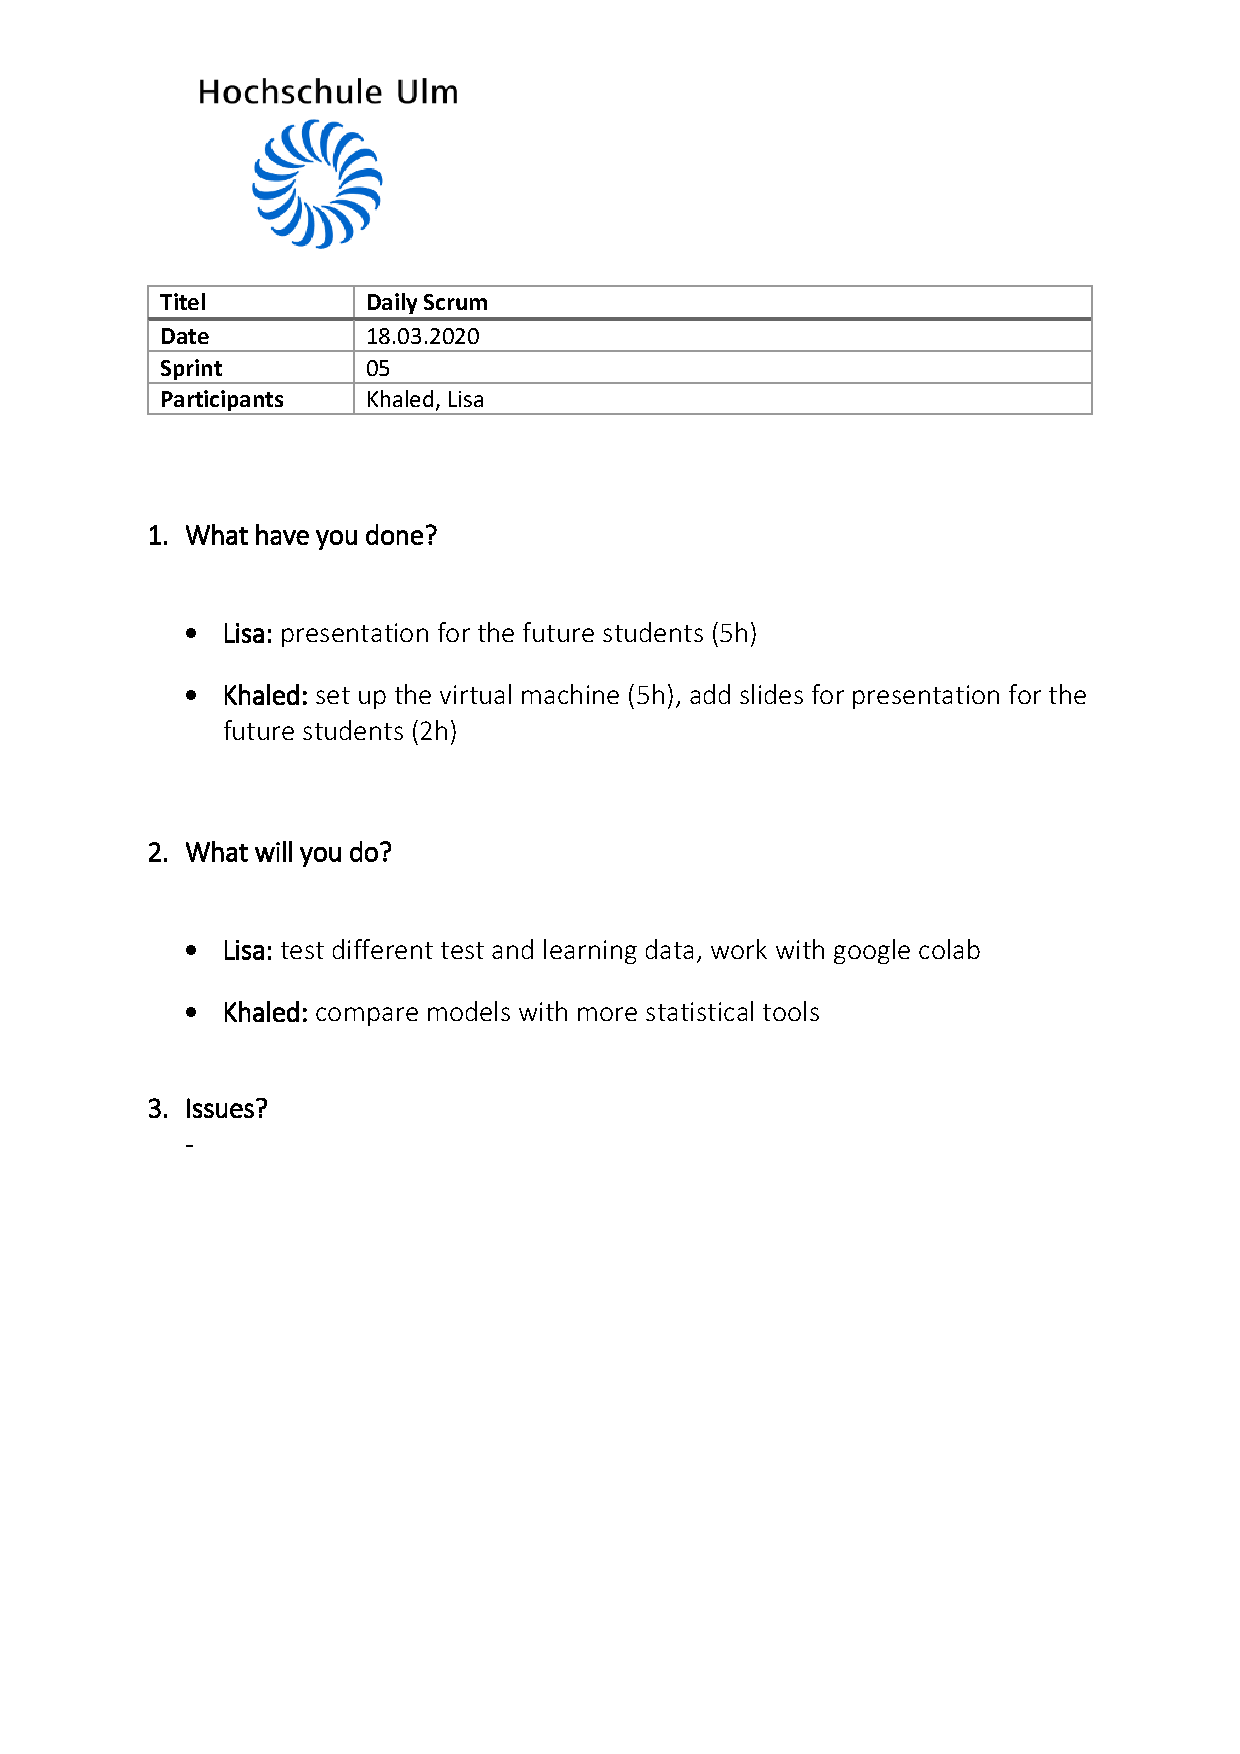
\includepdf[pages={1}]{pdf/Daily_Scrum_51.pdf}
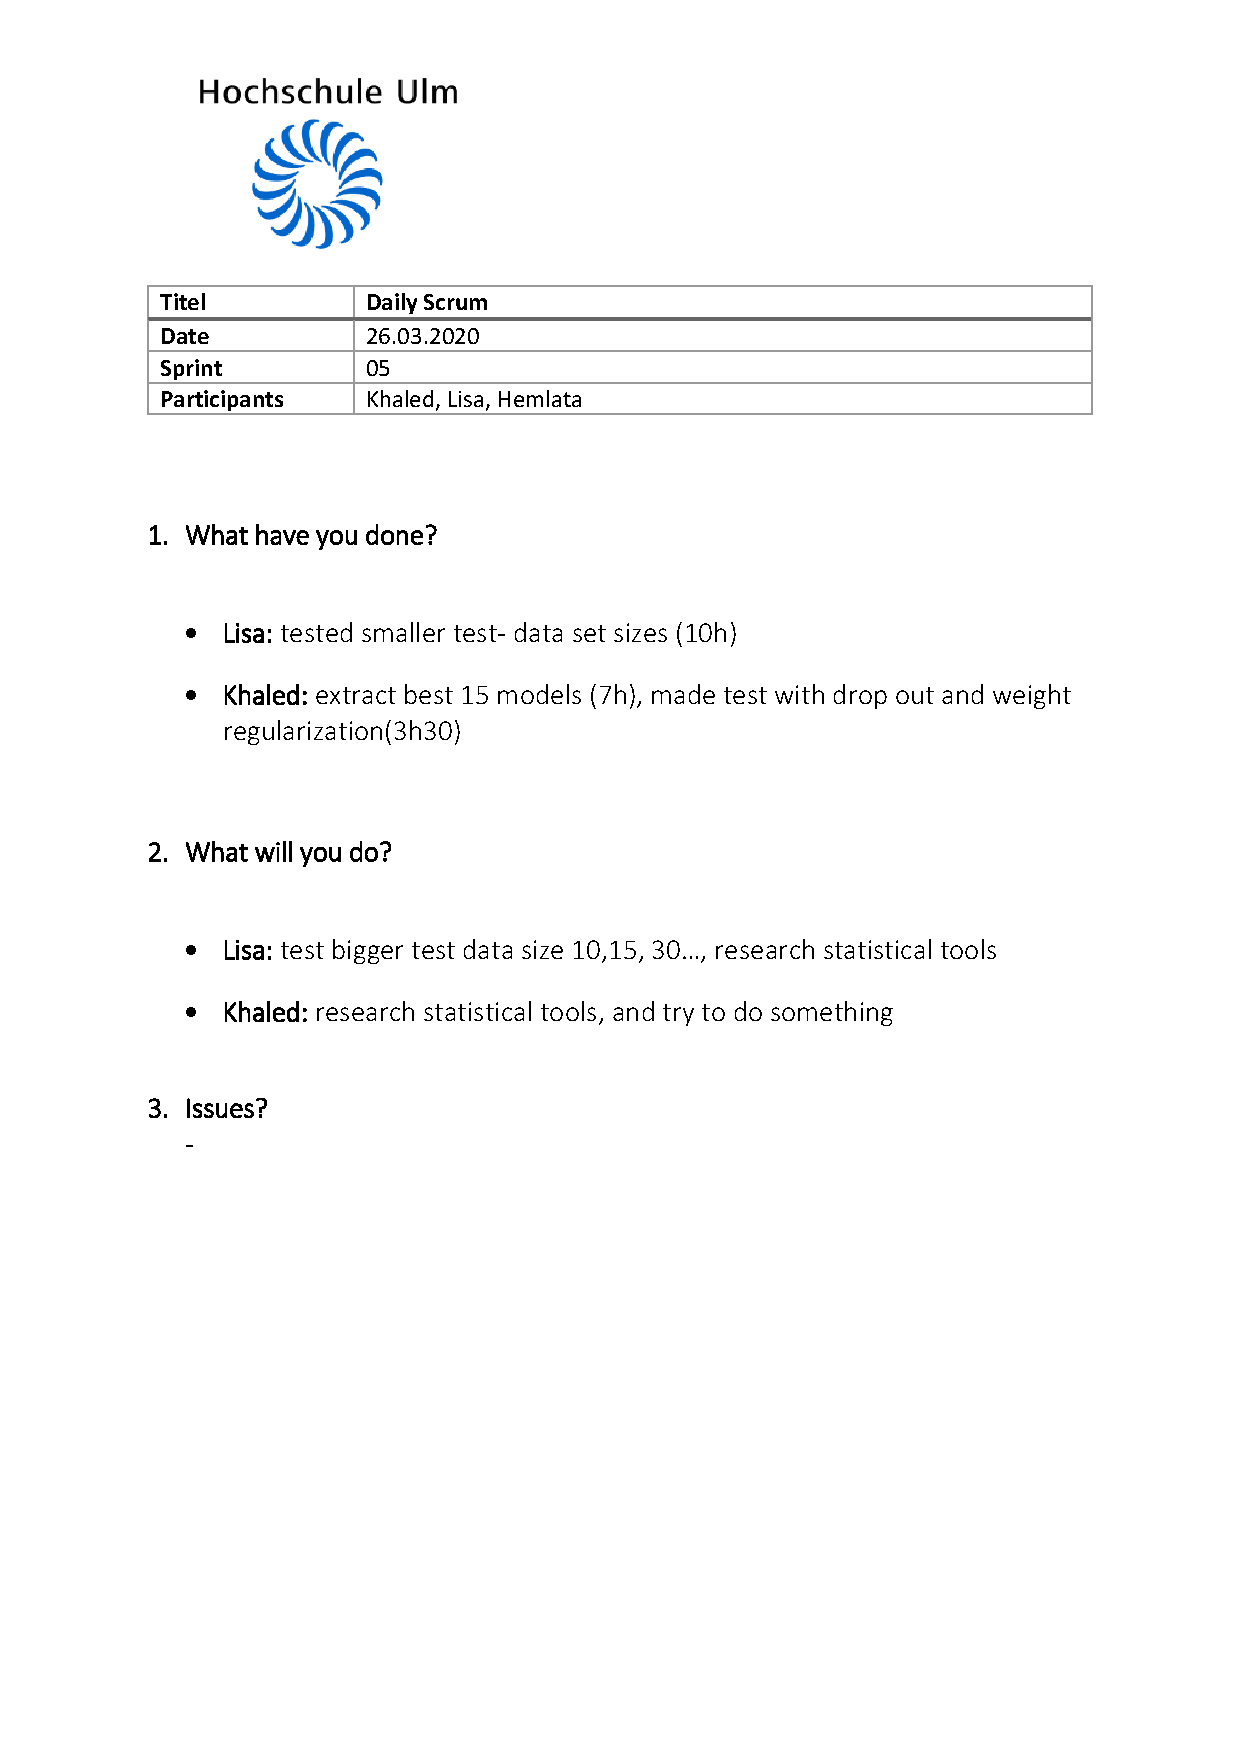
\includepdf[pages={1}]{pdf/Daily_Scrum_52.pdf}
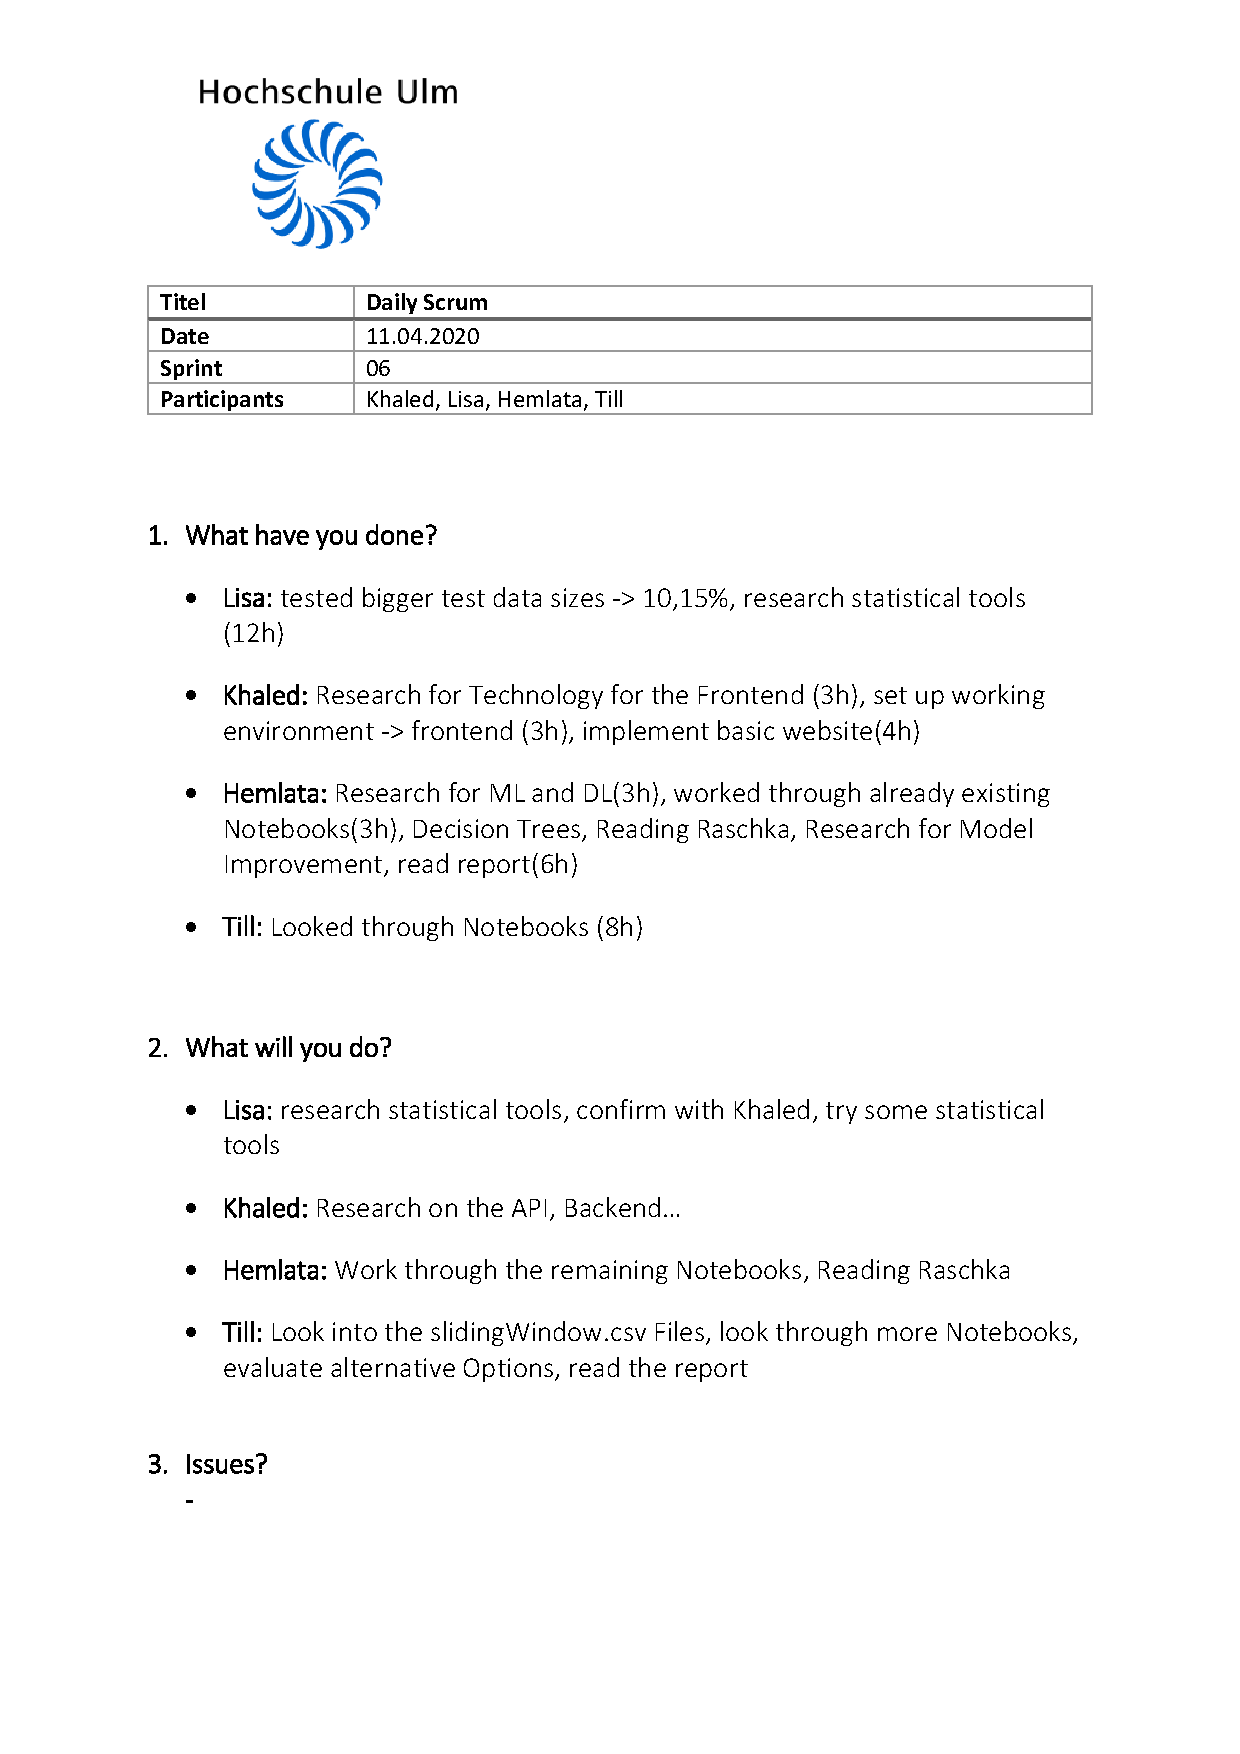
\includepdf[pages={1}]{pdf/Daily_Scrum_61.pdf}
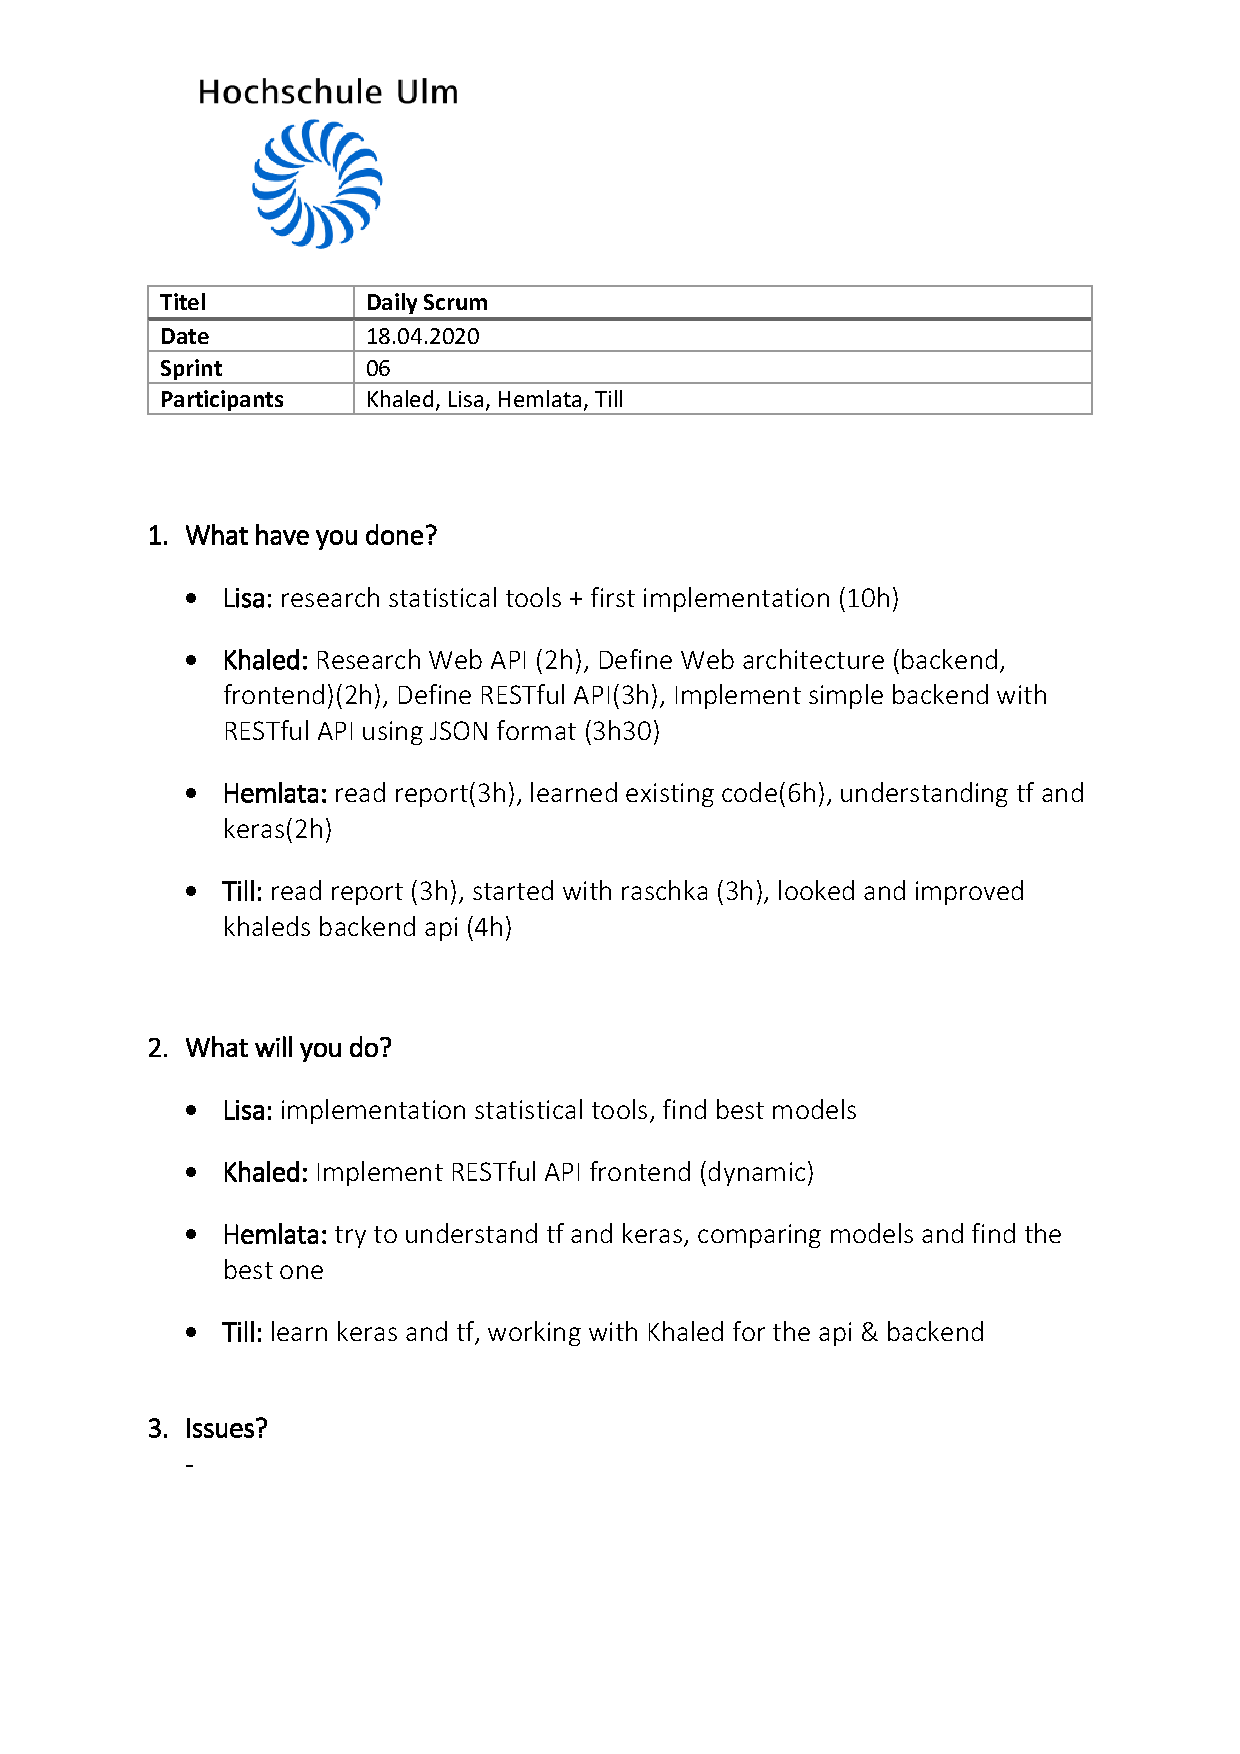
\includepdf[pages={1}]{pdf/Daily_Scrum_62.pdf}
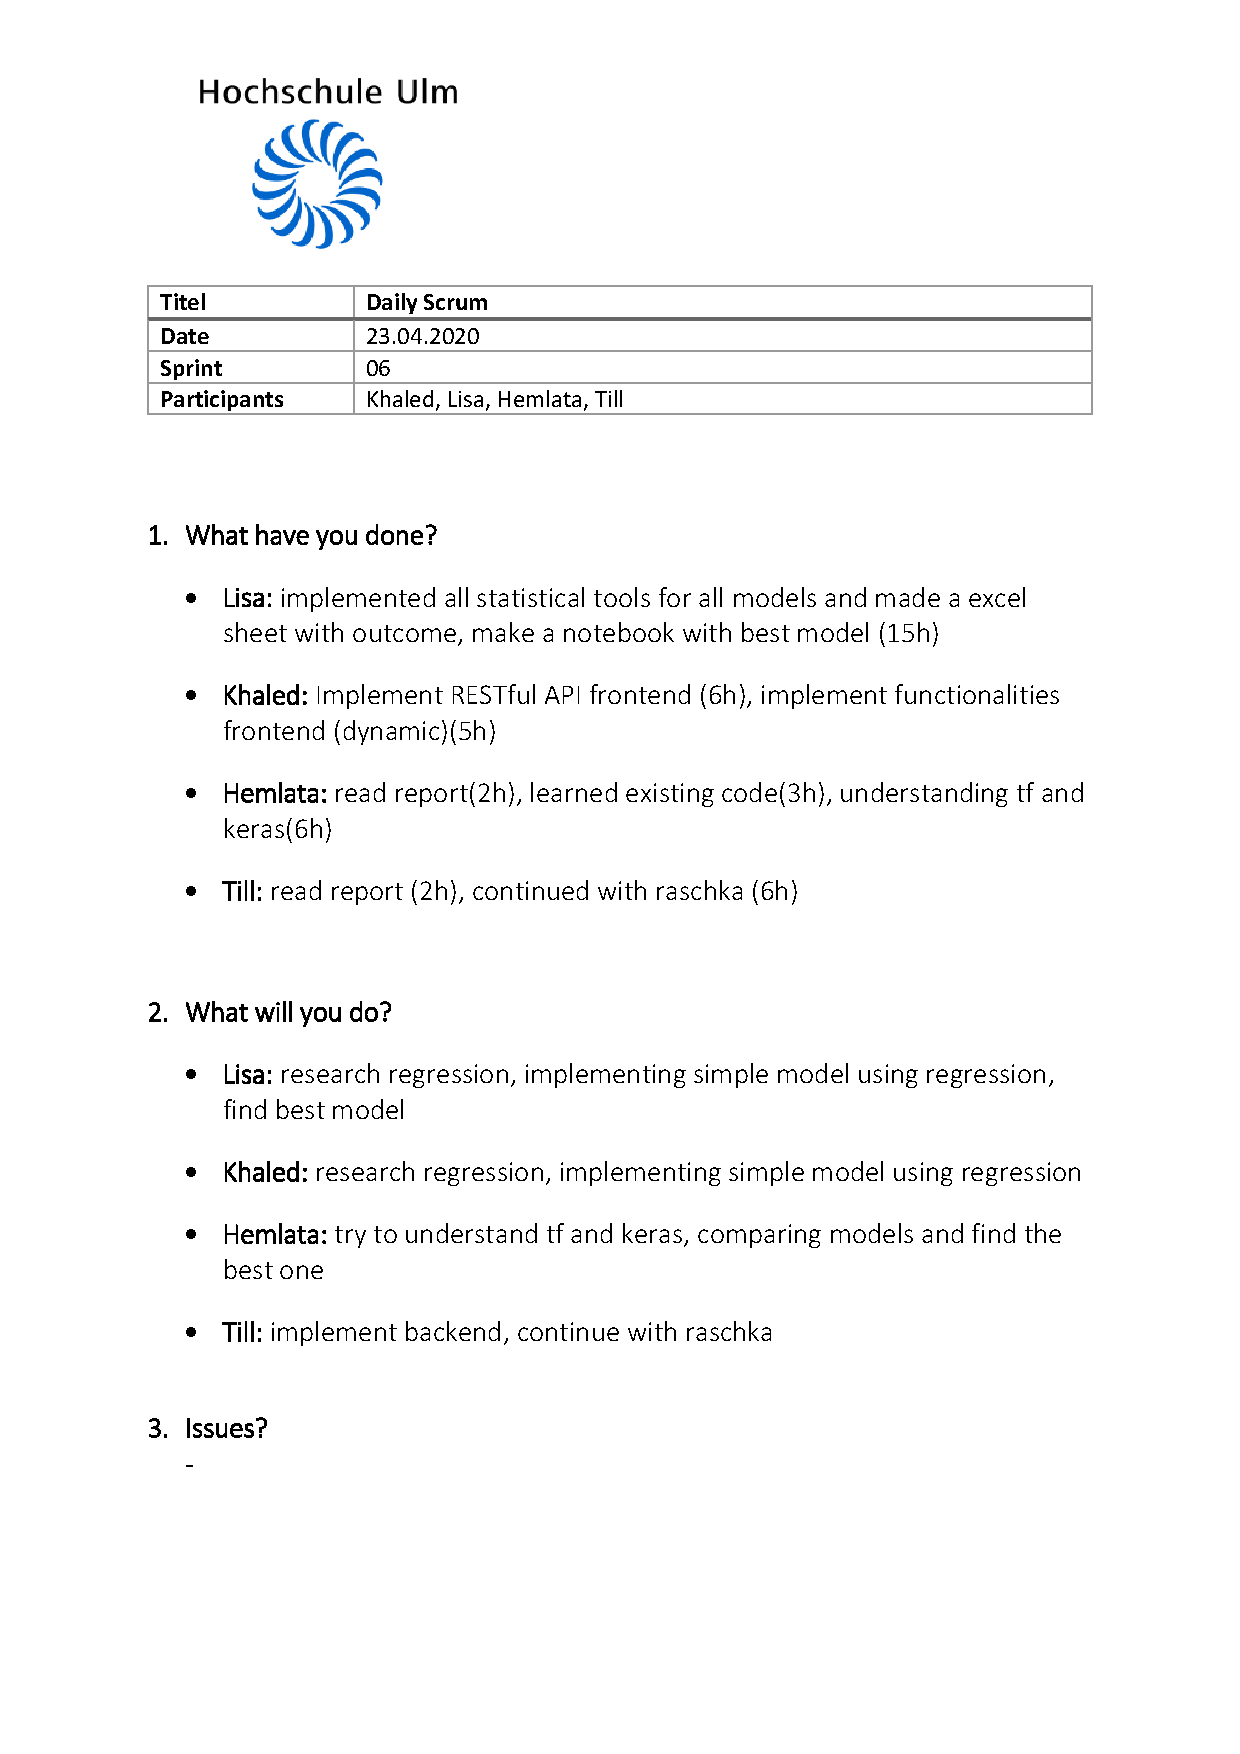
\includepdf[pages={1}]{pdf/Daily_Scrum_63.pdf}
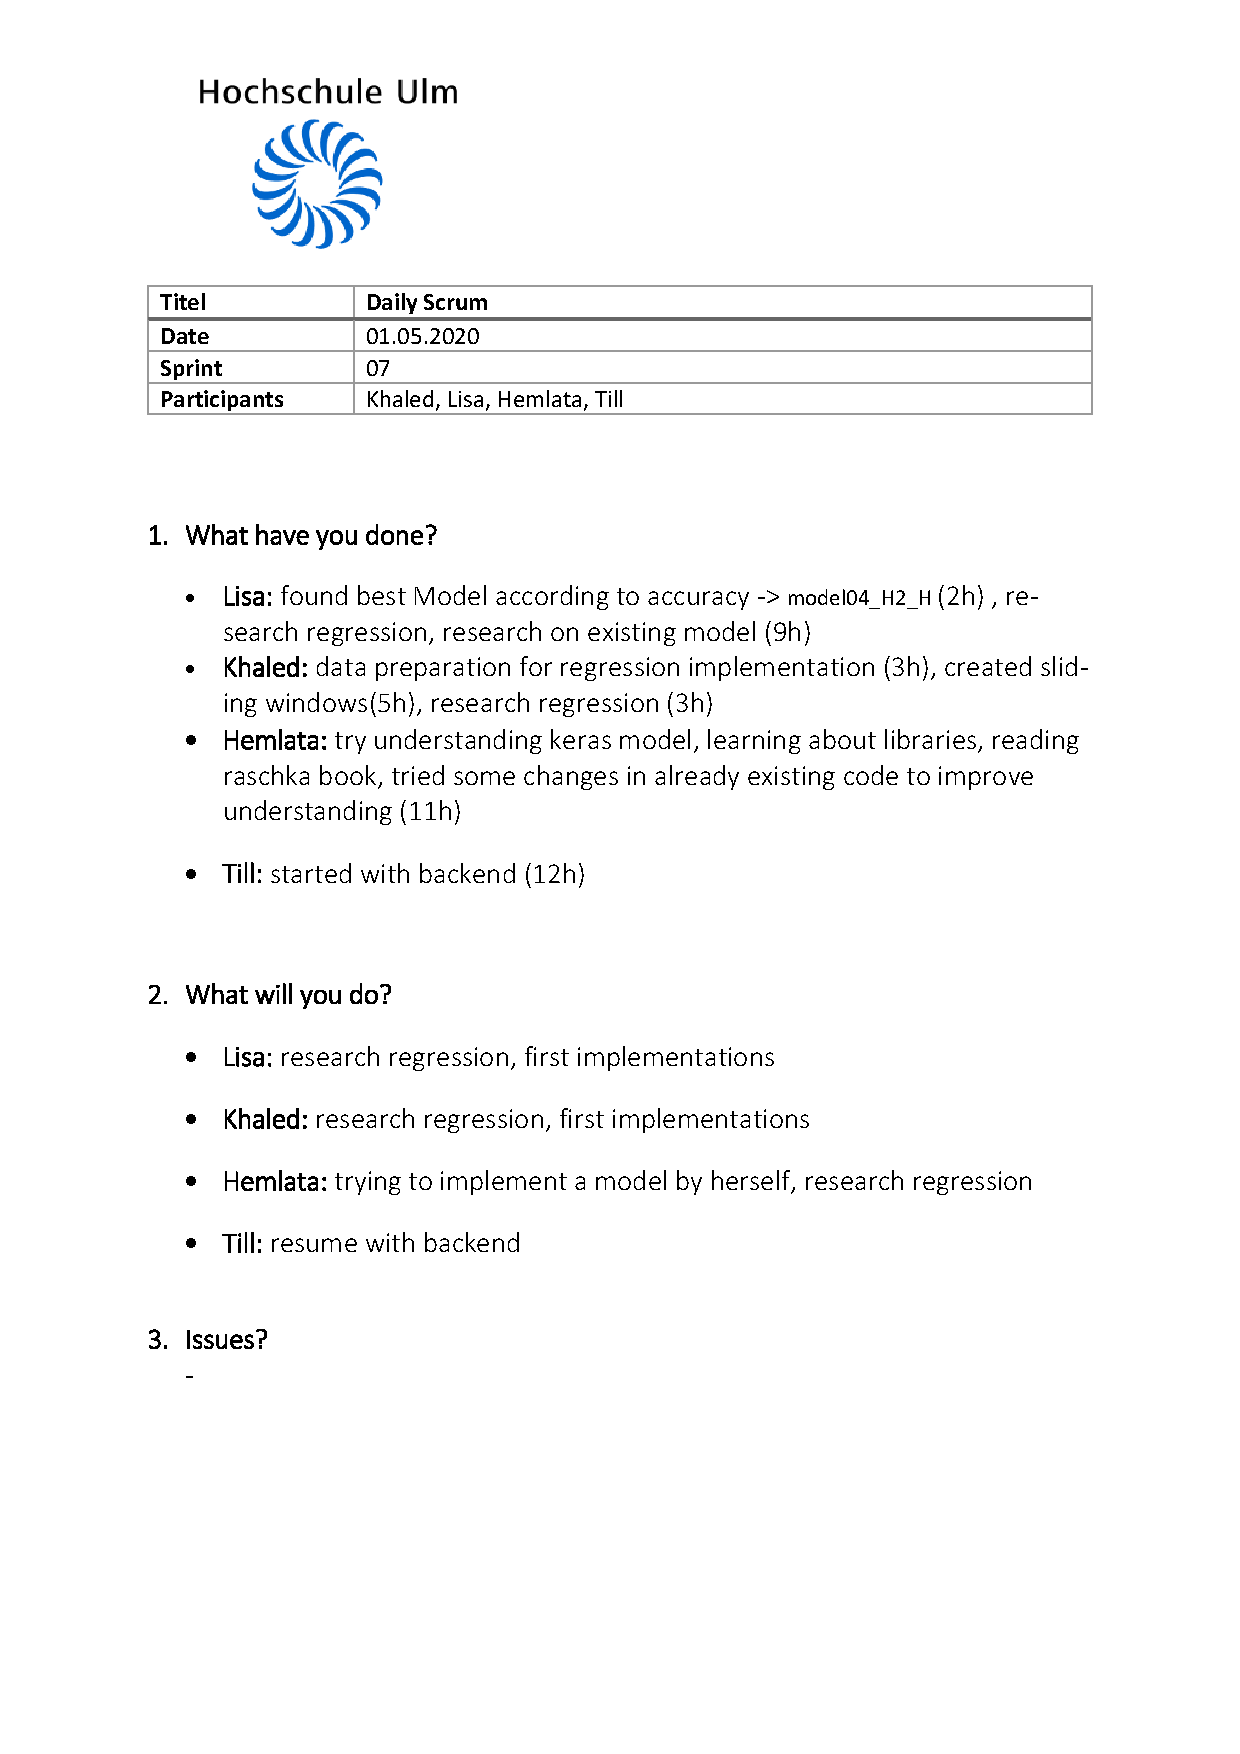
\includepdf[pages={1}]{pdf/Daily_Scrum_71.pdf}
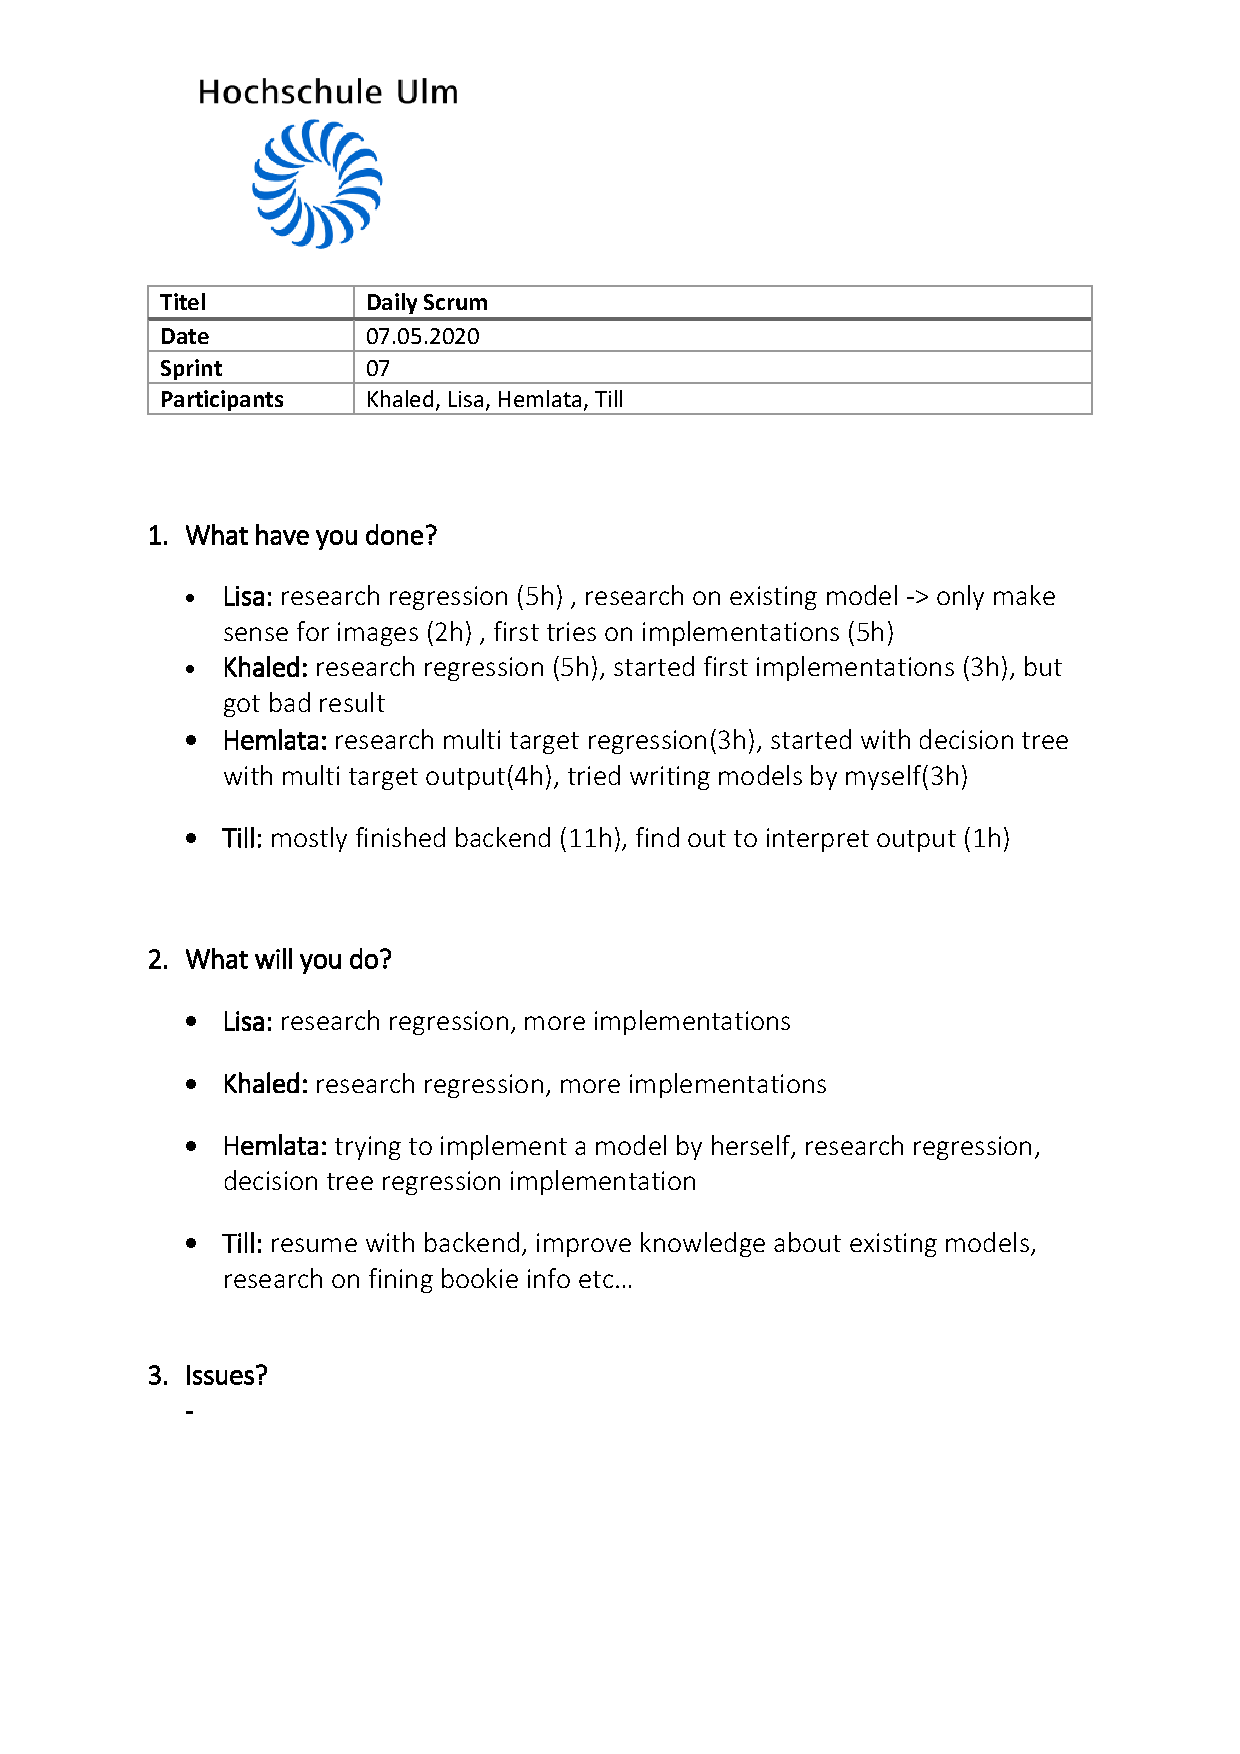
\includepdf[pages={1}]{pdf/Daily_Scrum_72.pdf}
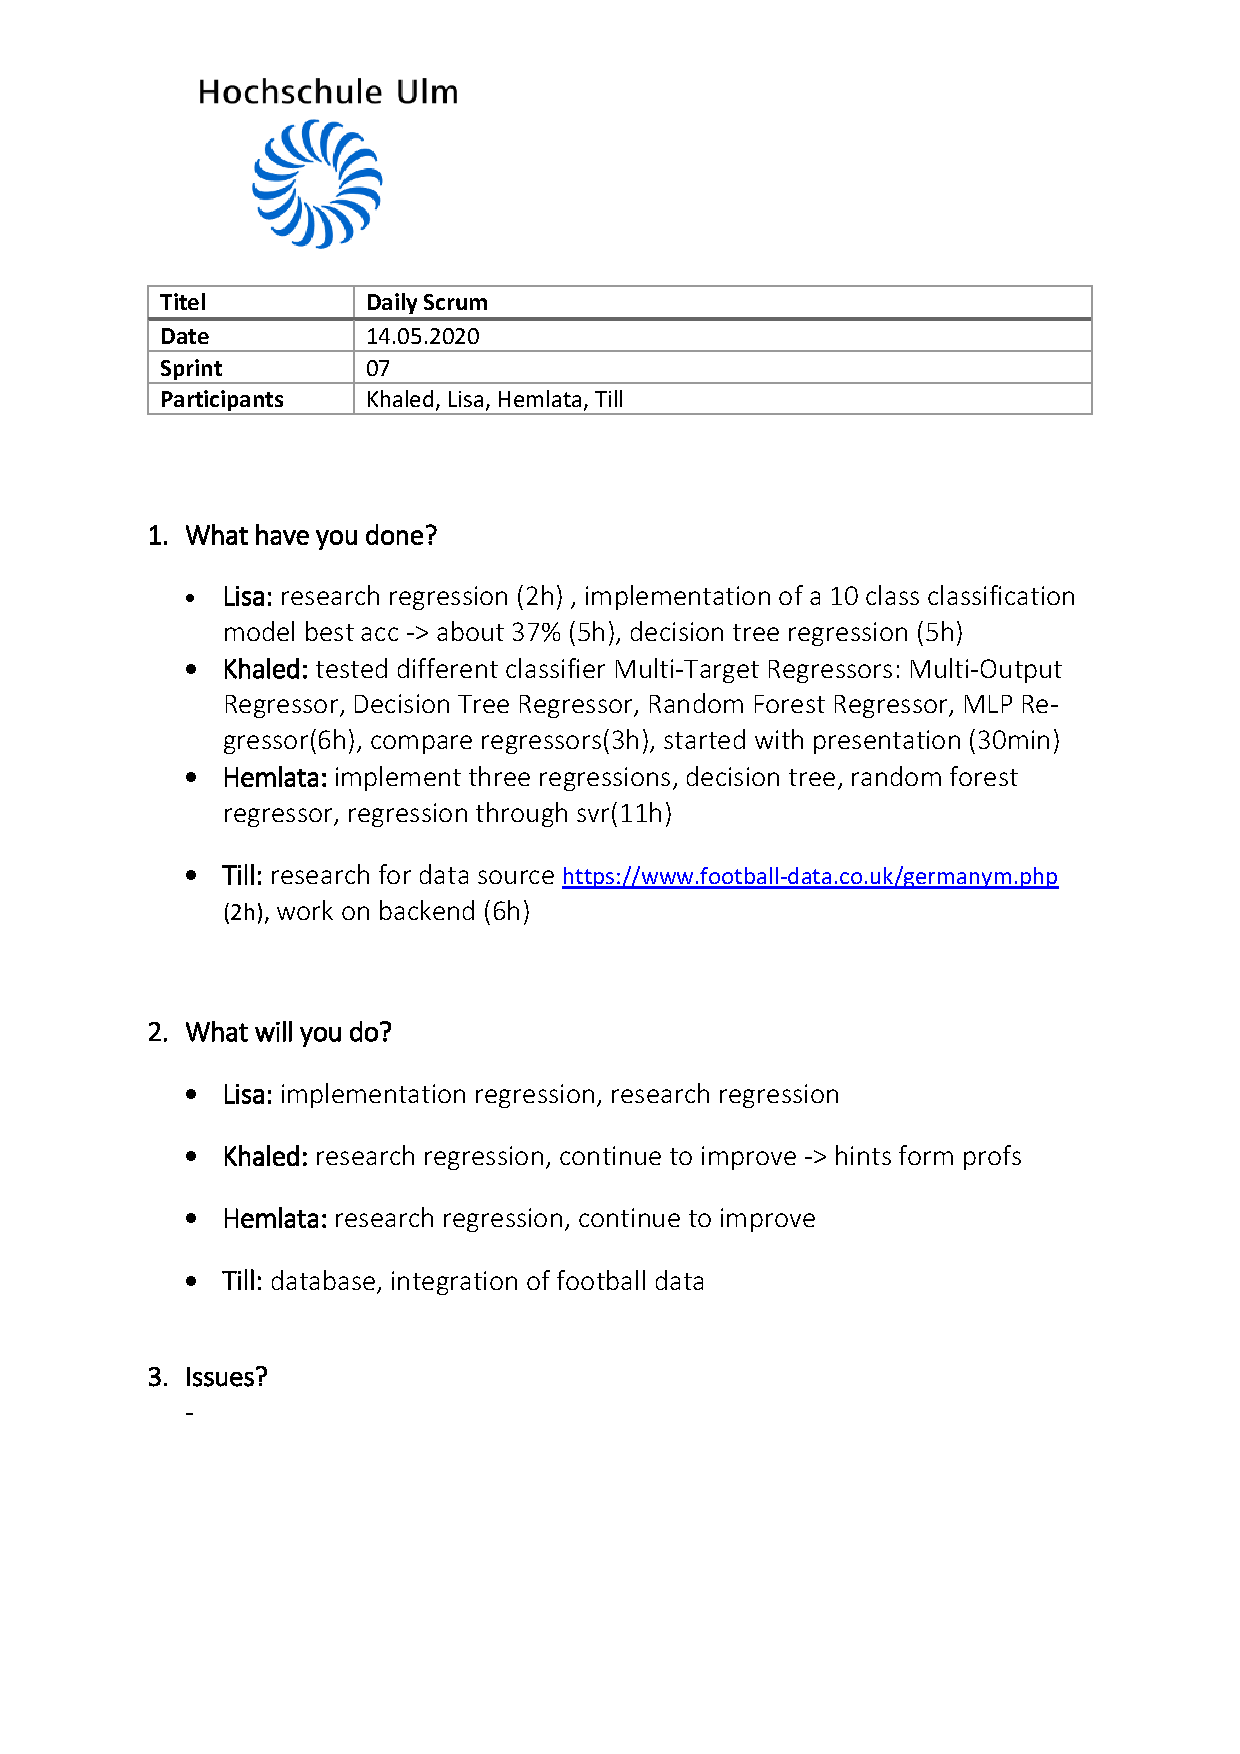
\includepdf[pages={1}]{pdf/Daily_Scrum_73.pdf}
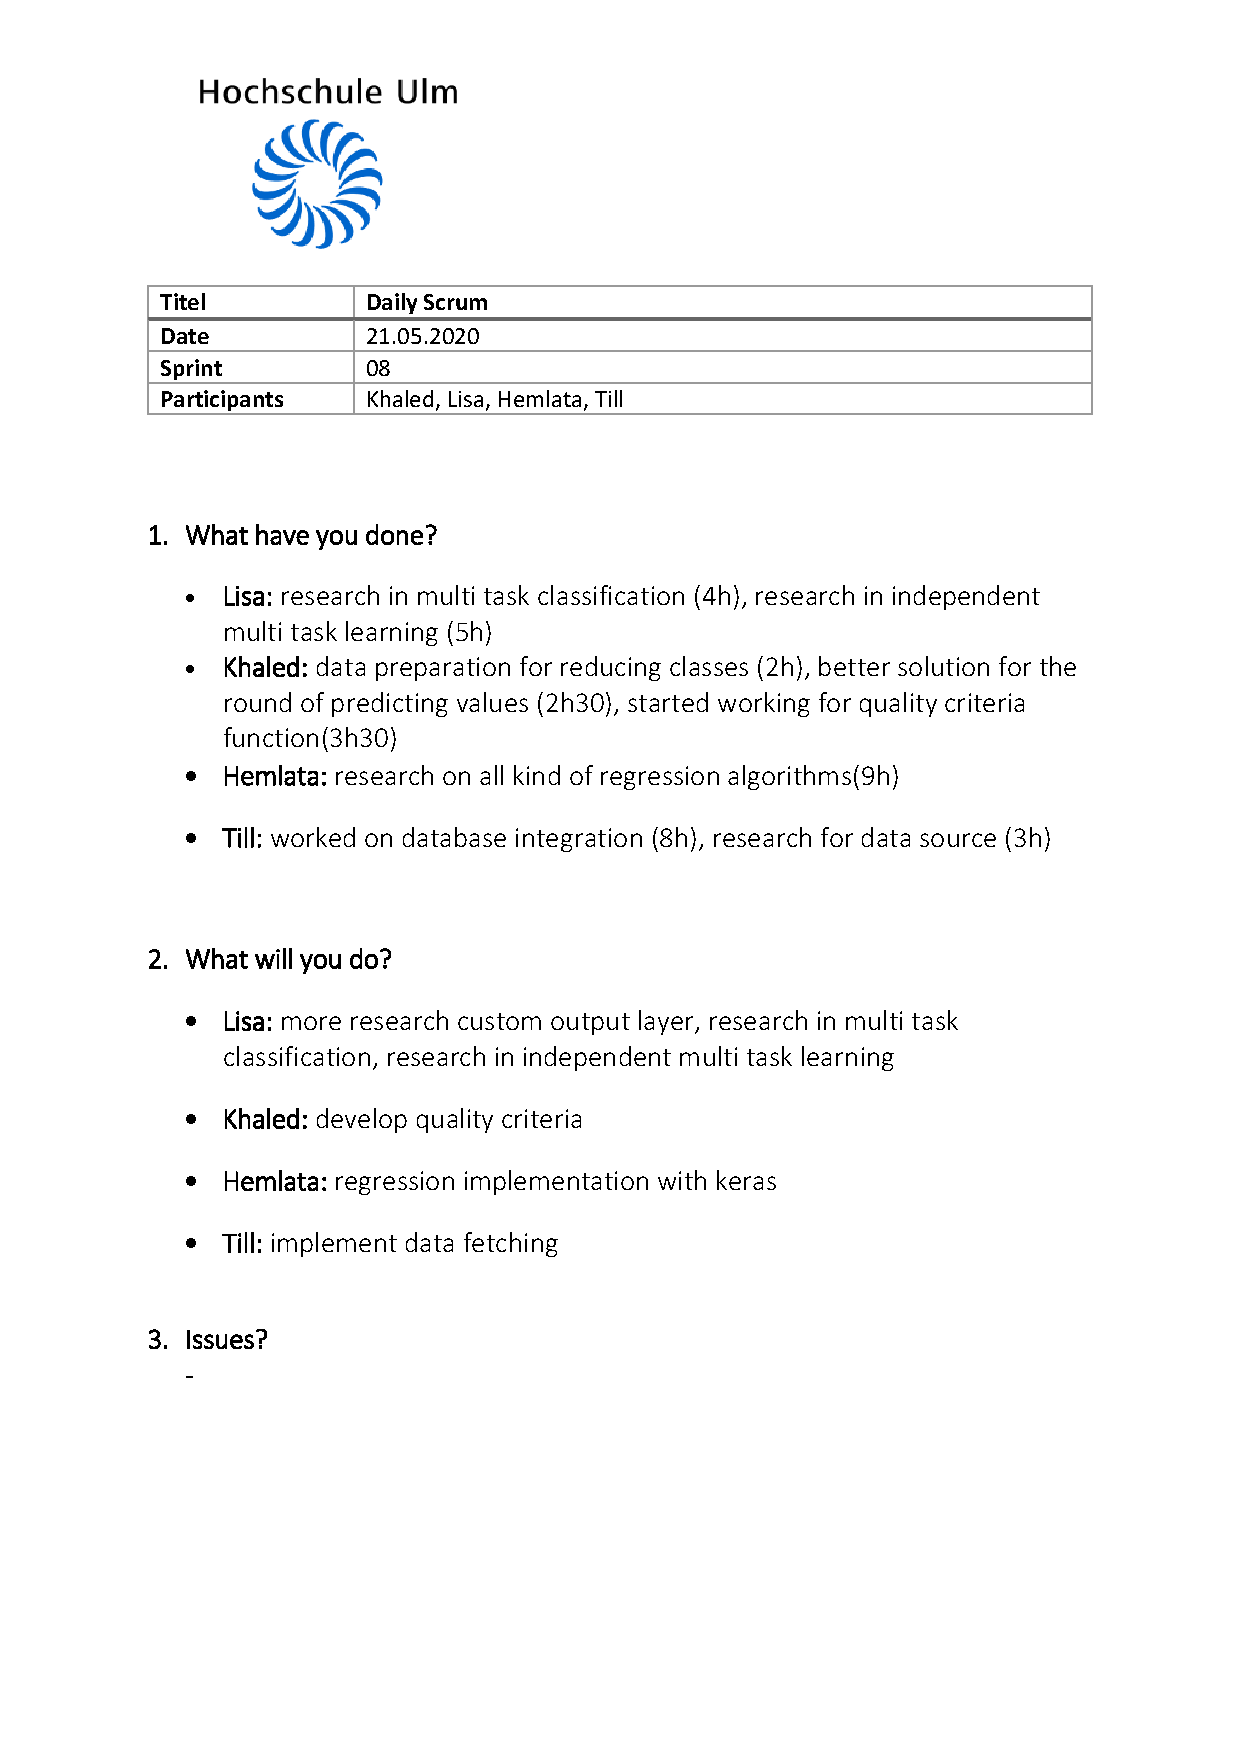
\includepdf[pages={1}]{pdf/Daily_Scrum_81.pdf}
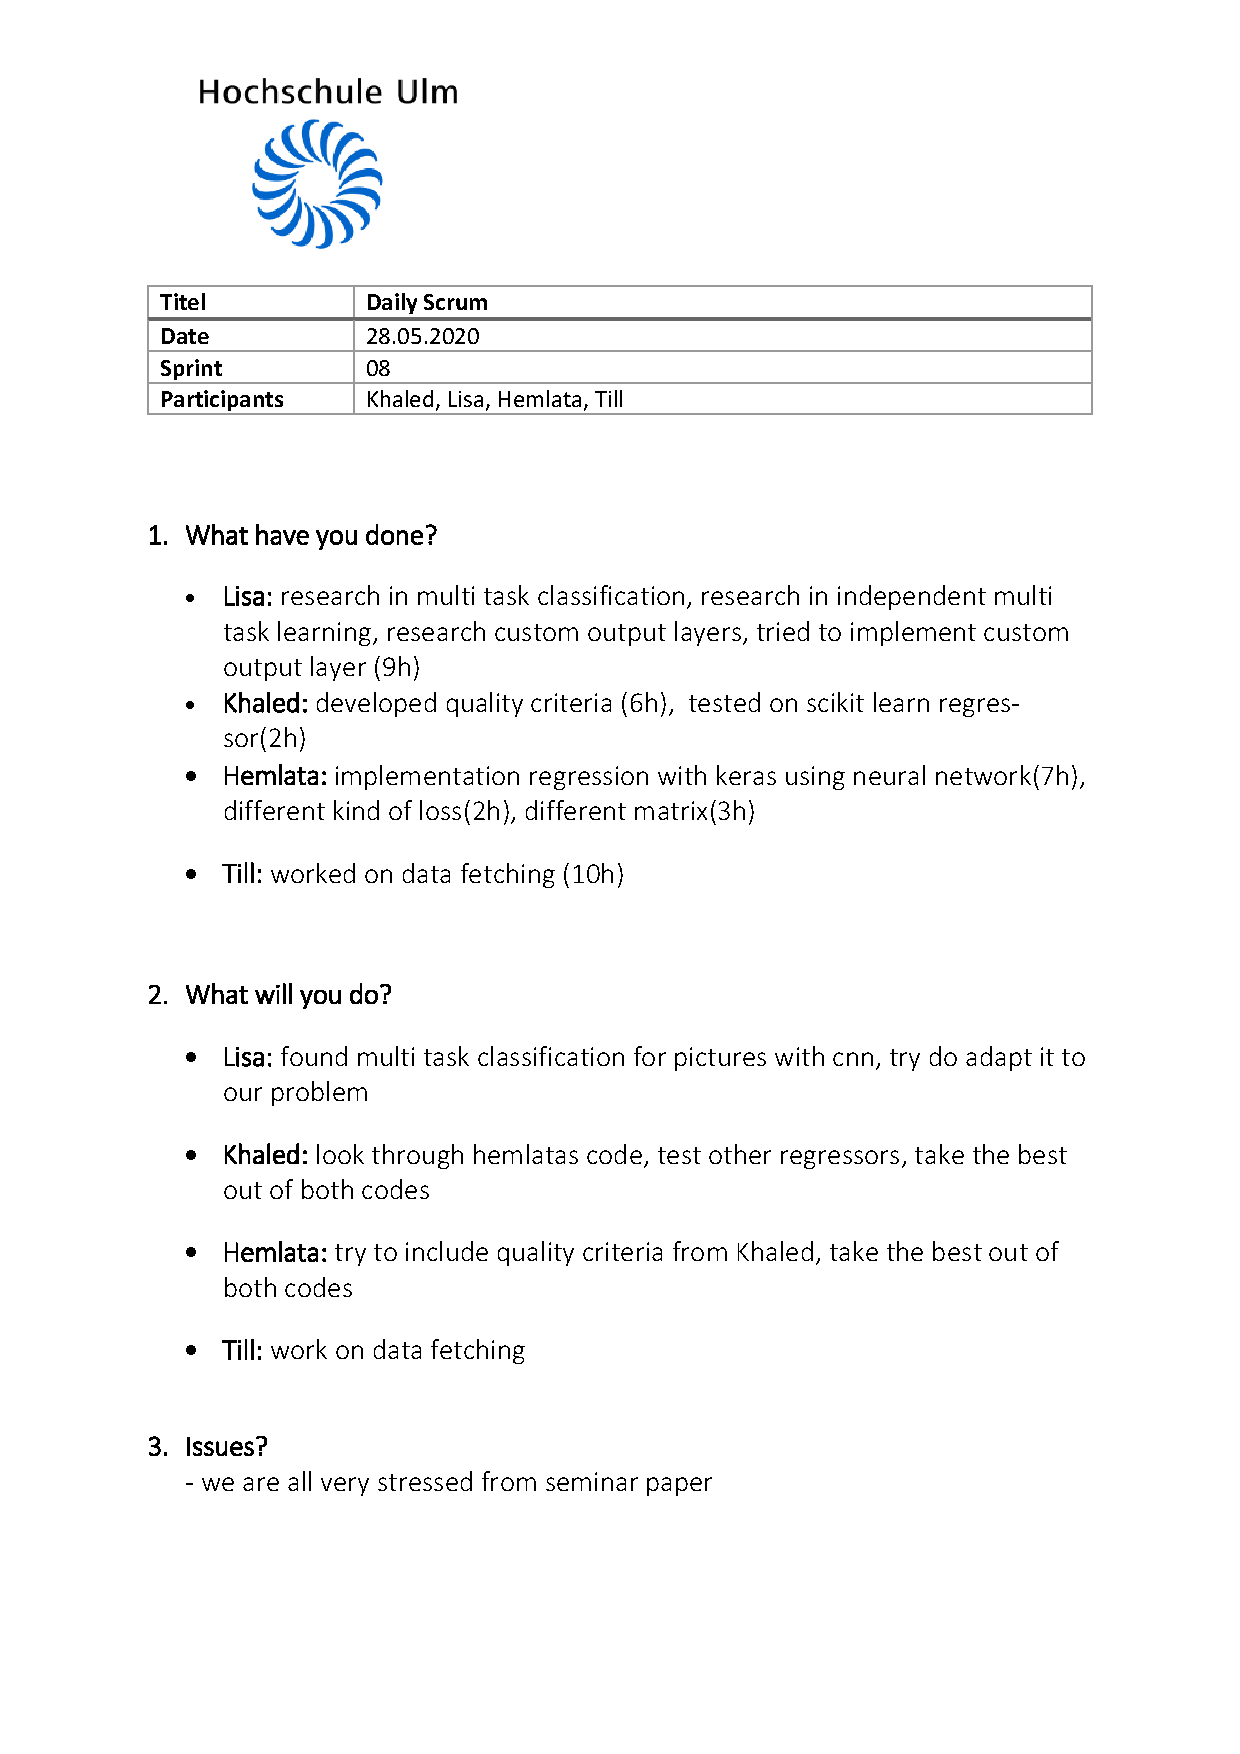
\includepdf[pages={1}]{pdf/Daily_Scrum_82.pdf}
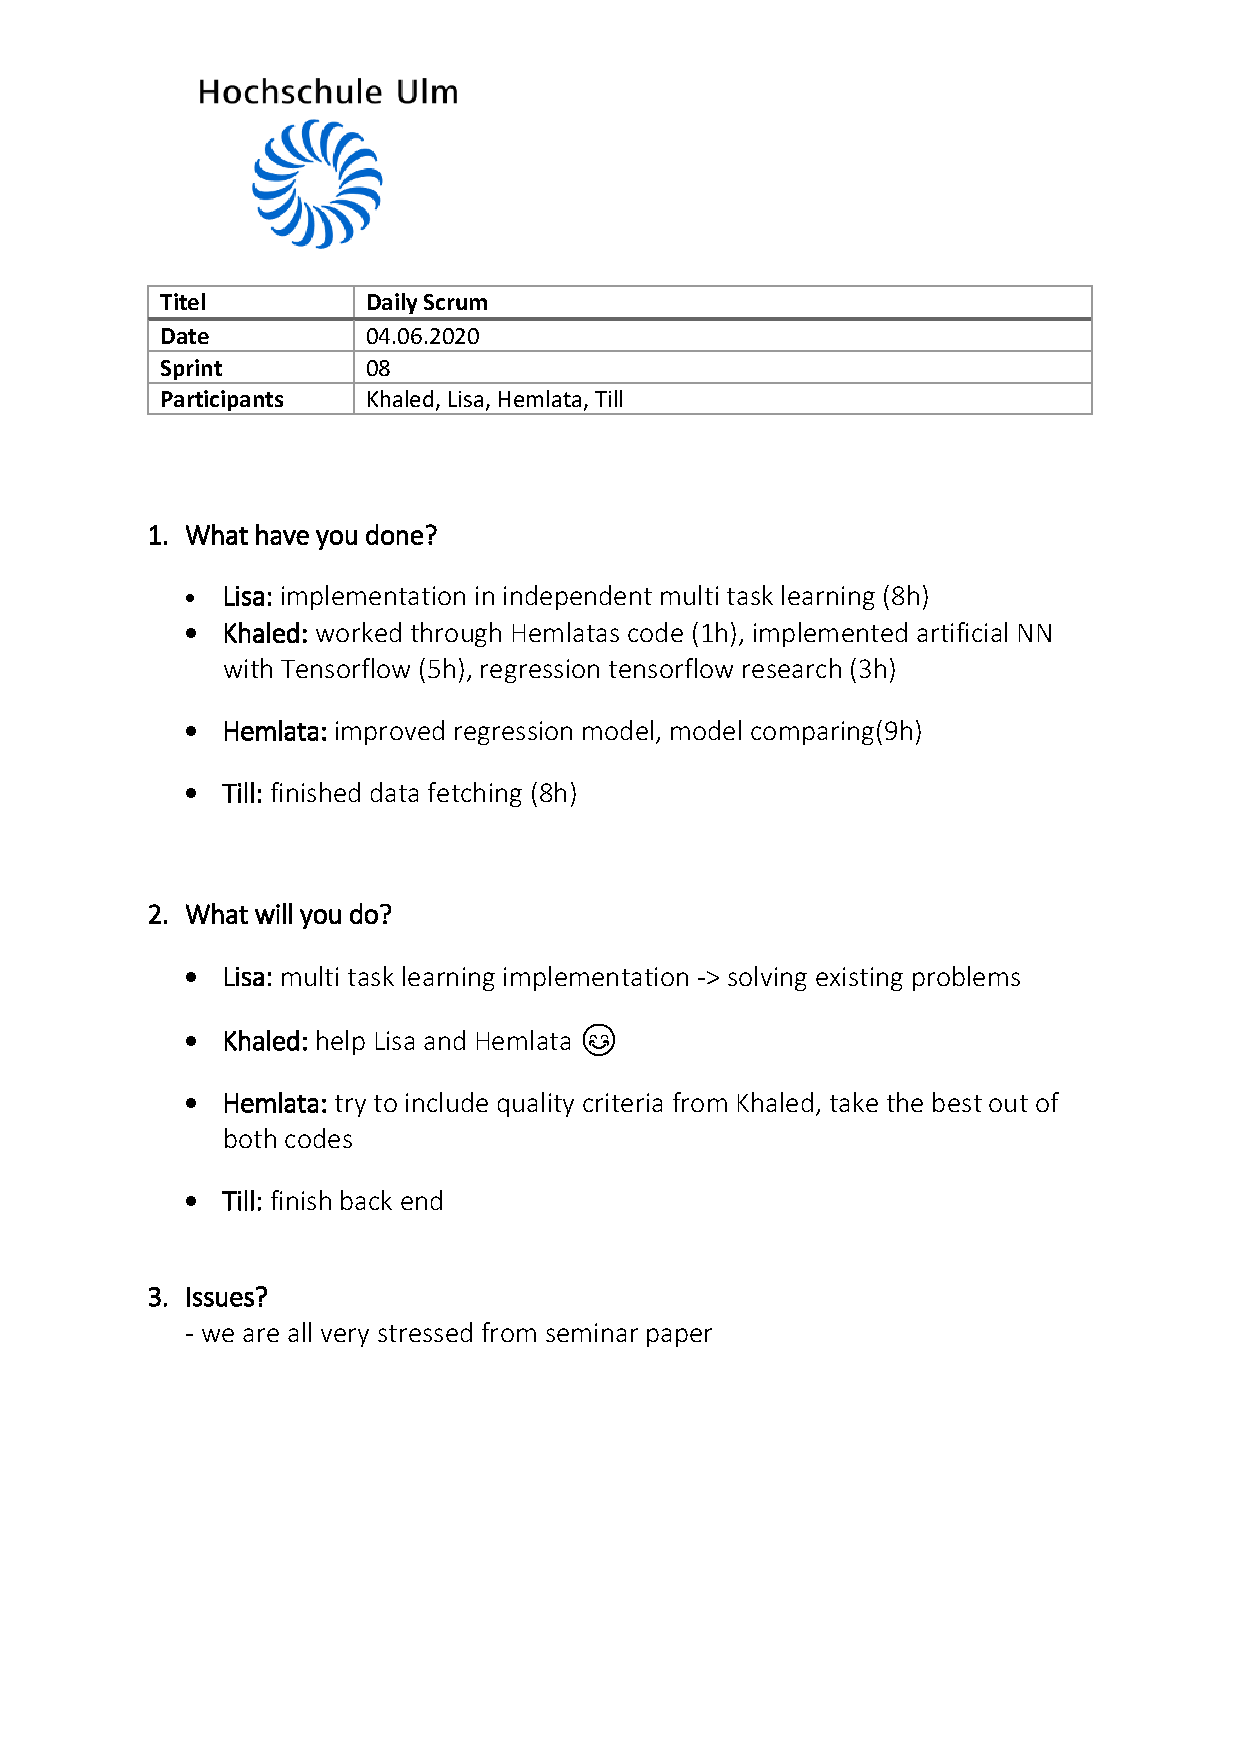
\includepdf[pages={1}]{pdf/Daily_Scrum_83.pdf}
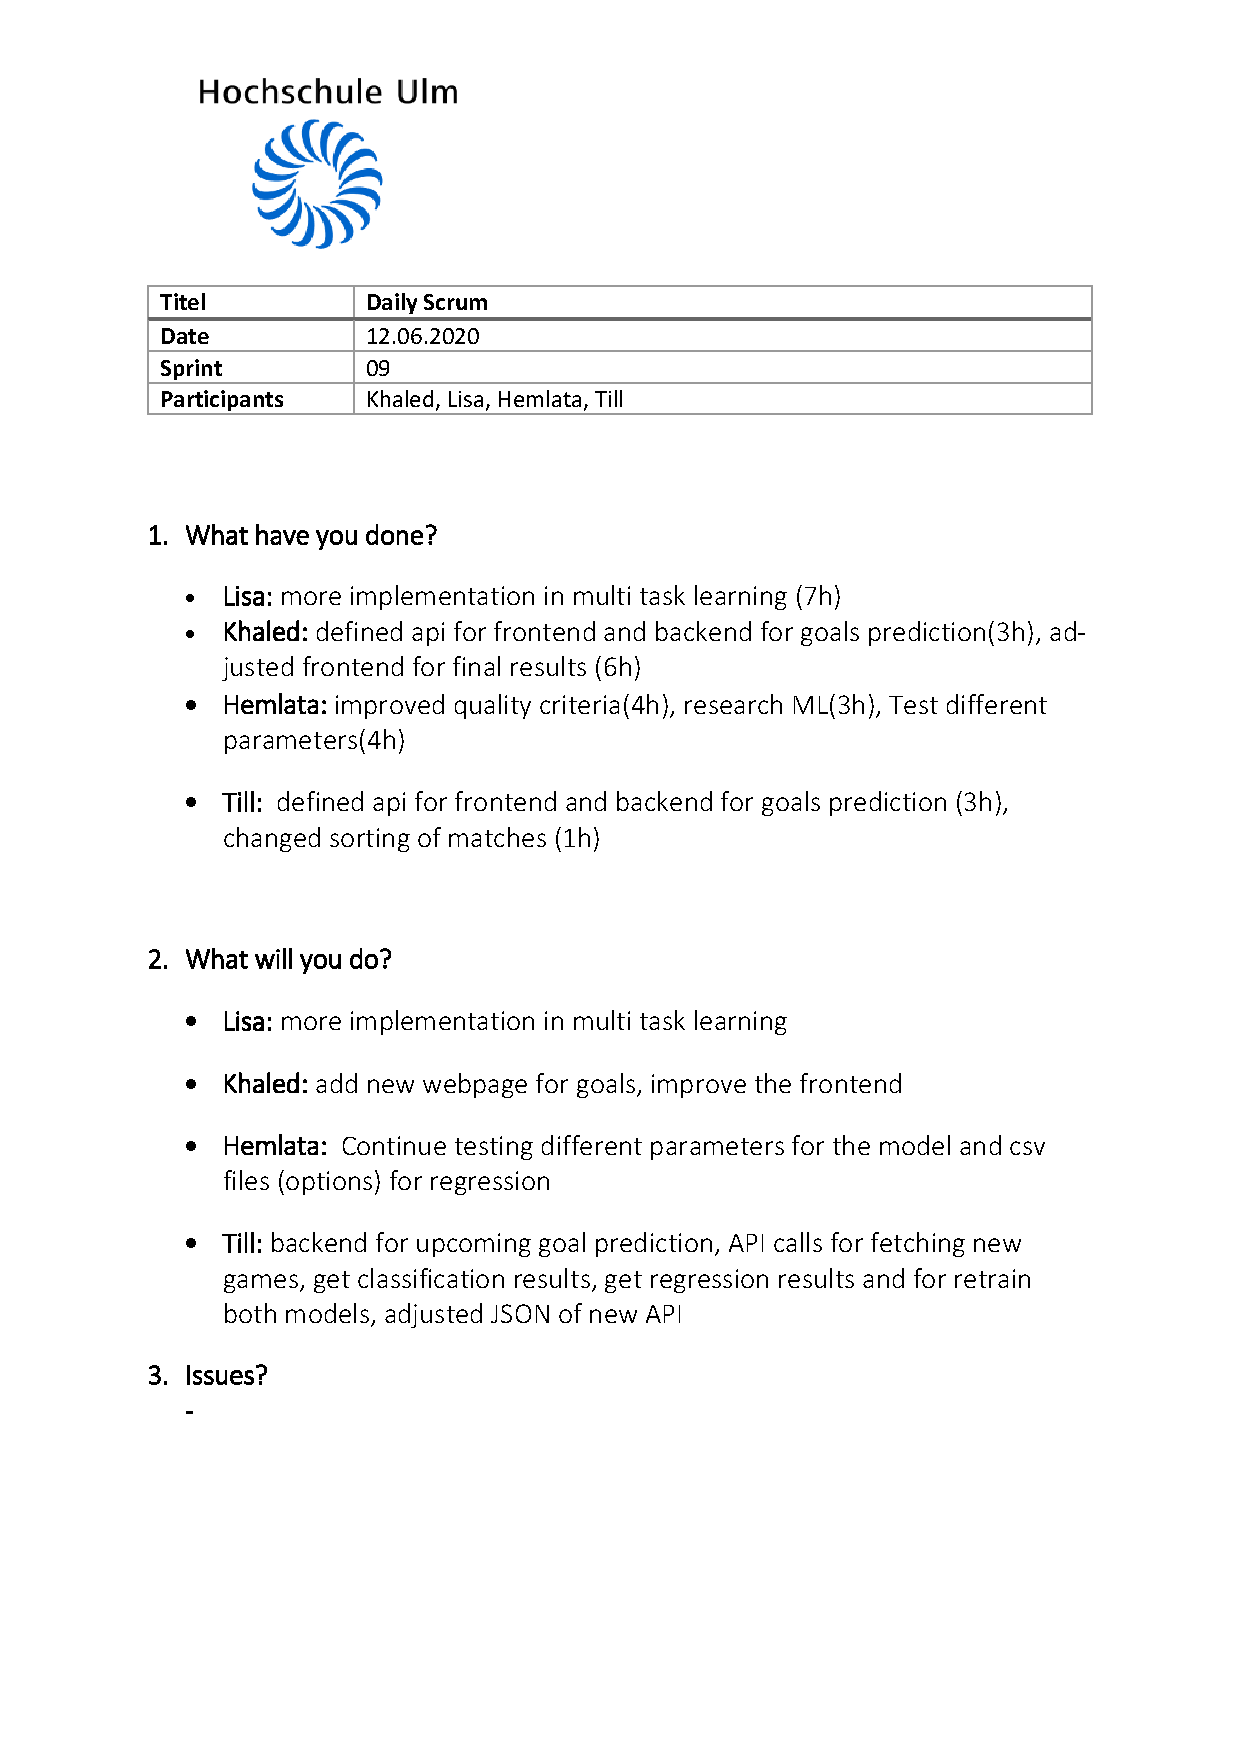
\includepdf[pages={1}]{pdf/Daily_Scrum_91.pdf}
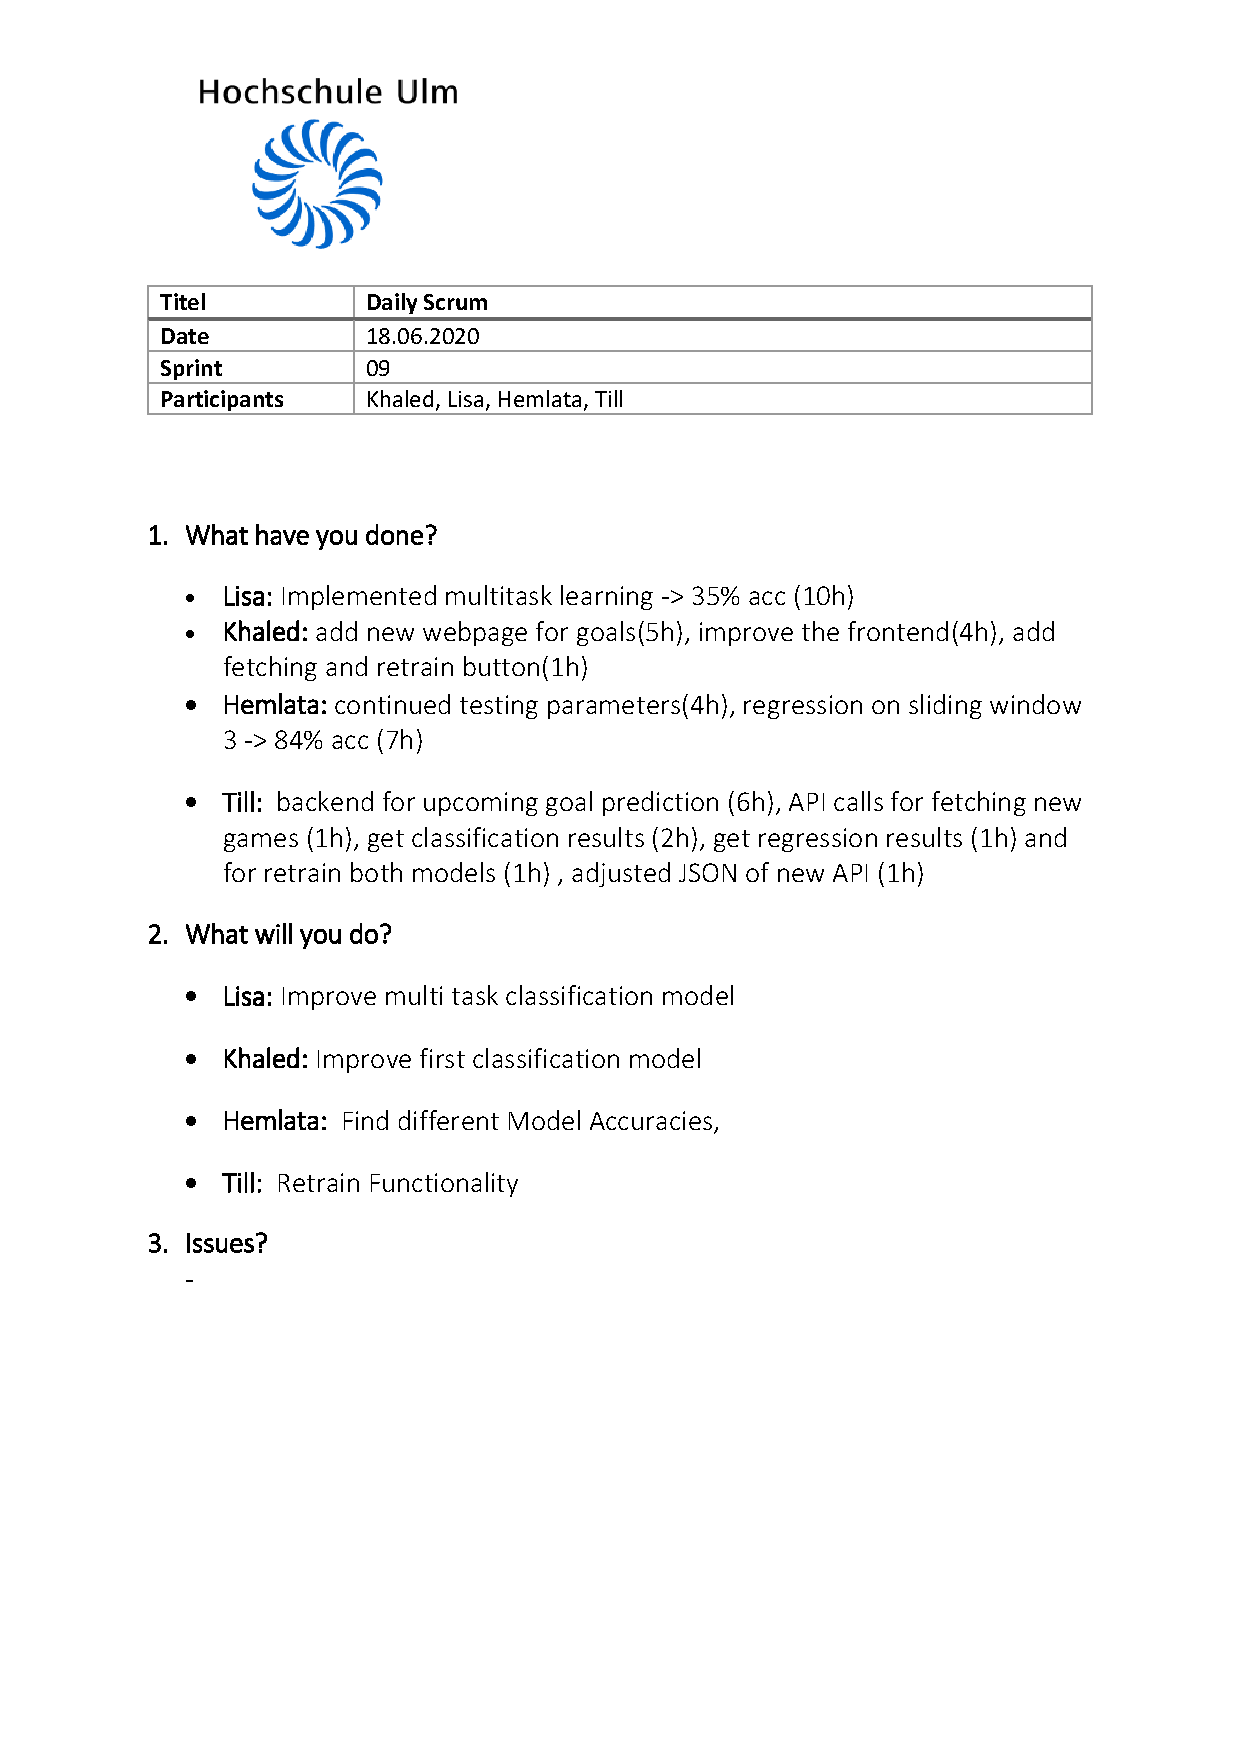
\includepdf[pages={1}]{pdf/Daily_Scrum_92.pdf}
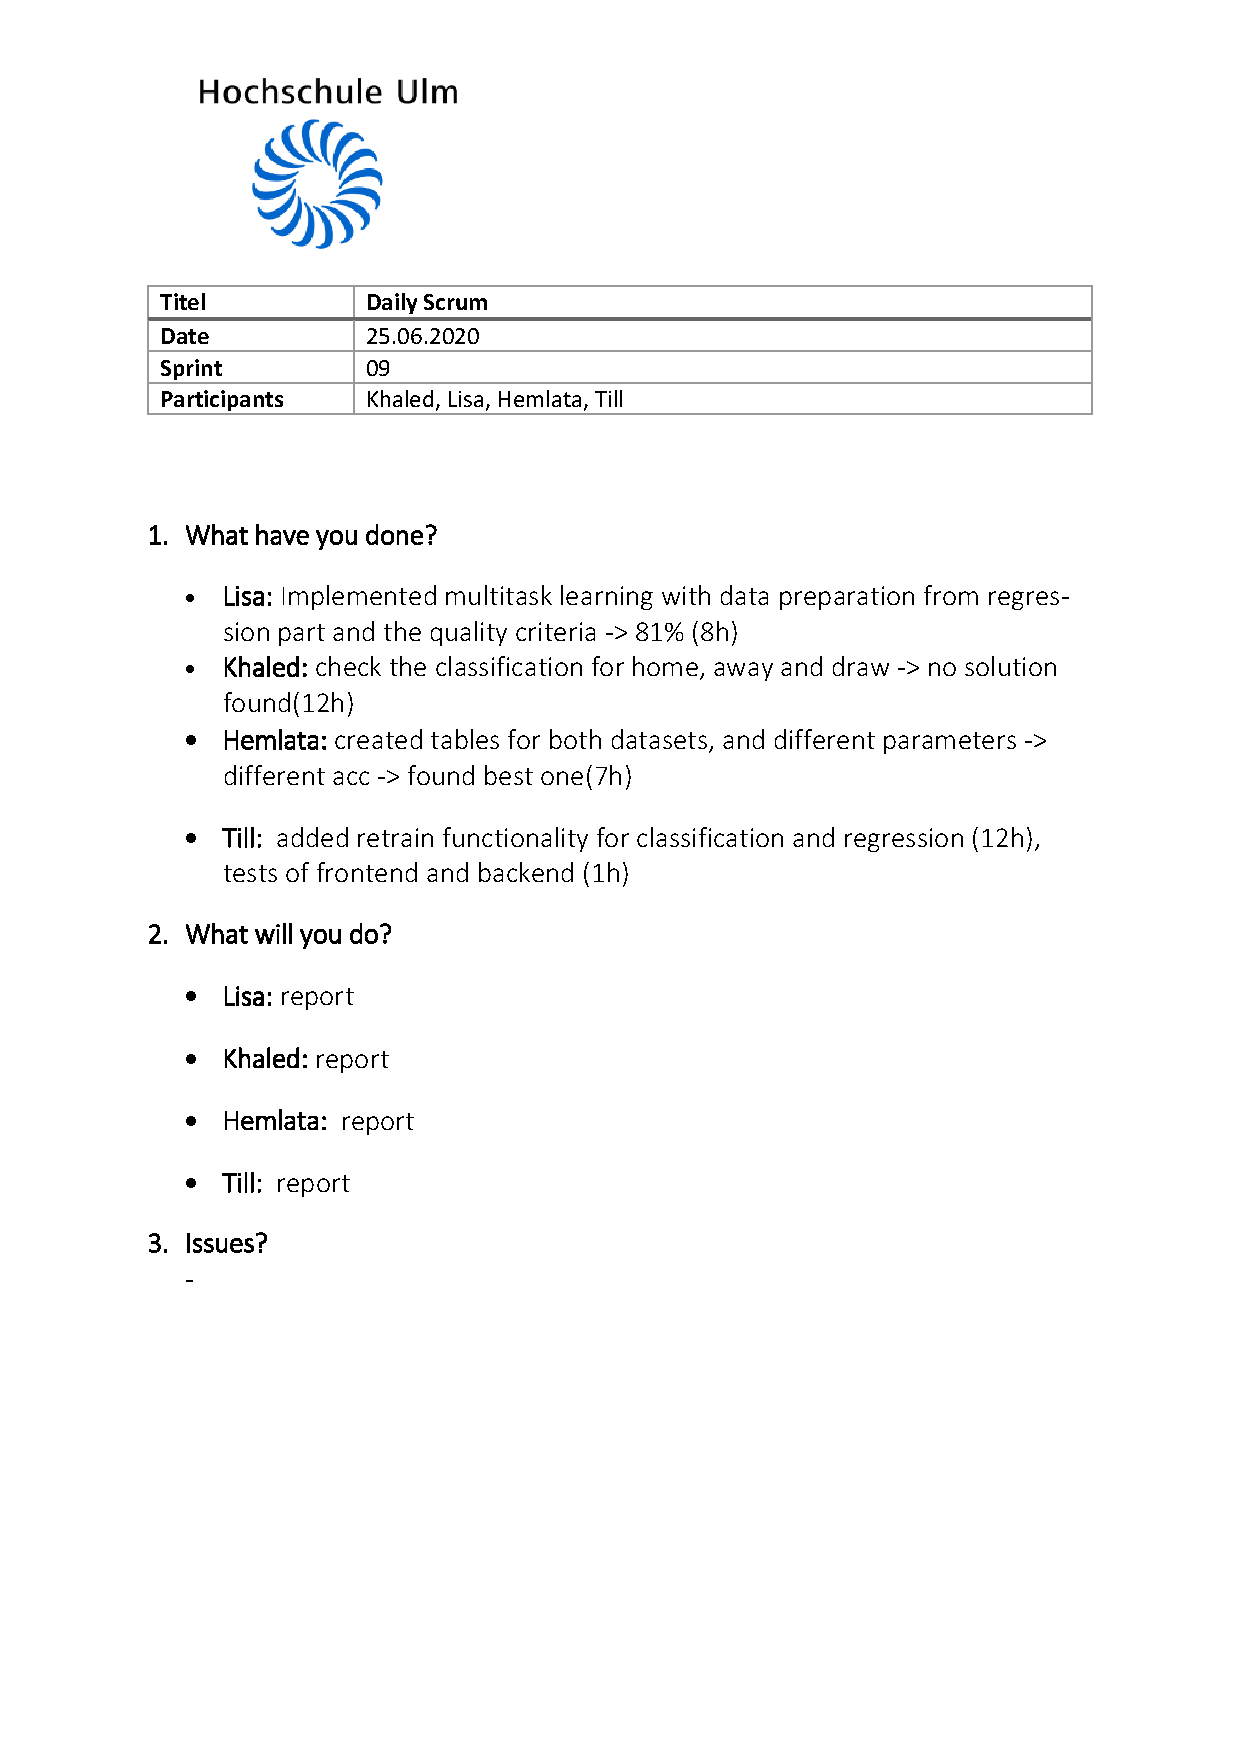
\includepdf[pages={1}]{pdf/Daily_Scrum_93.pdf}

%\newpage
%\section{ Report of First Semester}
%\label{section:appendix_c}
%\newpage

	
\end{document}
